\documentclass[11pt,a4paper]{book}
\usepackage{pdfpages}
\pagenumbering{arabic} 
\usepackage{titlesec}
\usepackage{setspace}
\usepackage{graphicx}
\usepackage{wrapfig}
\usepackage{color,soul}
\usepackage[customcolors,shade]{hf-tikz}
\usepackage{amsmath}
\usepackage{amssymb}
\usepackage{graphicx}
\usepackage{subfig}
\usepackage{xcolor}
\usepackage{subfig}
\usepackage{sidecap}
\usepackage{appendix}
\usepackage{layout}
\usepackage{amsthm}
\usepackage[italian]{babel}
\usepackage{fancyhdr}
\pagestyle{fancy}
\fancyfoot[C]{\thepage}
\fancyhead[RO,LE]{\leftmark} 
\fancyhead[RE,LO]{}
\usepackage{hyperref}
\usepackage{bm}
\hypersetup{
    colorlinks=true,
    linkcolor=magenta,
    filecolor=magenta,      
    urlcolor=blue,
    pdftitle={Statistics and Probability},
    pdfpagemode=FullScreen,
    }

\urlstyle{same}



\theoremstyle{remark}
\newtheorem*{remark}{Osservazione}

\renewcommand{\baselinestretch}{1.3} 
\newtheorem{theorem}{Teorema}[section]
\newtheorem{corollary}{Corollario}[theorem]
\newtheorem{lemma}[theorem]{Lemma}
\newtheorem{definition}{Definizione}[section]
%\renewcommand\qedsymbol{$\blacksquare$}


\titleformat{\chapter}[display]
 {\bfseries\Large}
  {\filright\MakeUppercase{\chaptertitlename} \Huge\thechapter}
  {1ex}
  {\titlerule\vspace{1ex}\filleft}
  [\vspace{1ex}\titlerule]

\graphicspath{{/Users/giuliodilernia/Documents/Clasical-Mechanics-Notes/Classical_Mechanics_Notes/images/}}



\begin{document}
\includepdf[pages = 1,fitpaper]{copertina.pdf}
\tableofcontents
\begin{thebibliography}{6}
\bibitem{Appunti} 	Appunti del corso di meccanica classica tenuto dal professore Falqui Gregorio nell'anno 2022-2023
\bibitem{goldstein:mechanics} Meccanica Classica, Herbert Goldstein, Ed. Zanichelli 2005 
\bibitem{Arn} Metodi Matematica Della Meccanica Classica, Vladimir Igorevic Arnold, Ed. Editori Riuniti 2010
\bibitem{arnold} Ordinary Differential Equation,  Vladimir Igorevic Arnold, Ed. Springer 1992
\bibitem{Tong} Lecture of Classical Mechanics for Oxford Course in Classical Mechanics, David Tong \url{https://www.damtp.cam.ac.uk/user/tong/dynamics.html}
\bibitem{Landau} Fisica Teorica 1 Meccanica, Lev D. Landau, Ed. Editori Riuniti 2010
\bibitem{finch} Analyical Mechanics, Hand,Finch, Ed. Cambridge University Press 1998
\end{thebibliography}

\setcounter{chapter}{0}
\chapter{Leggi del Moto di Newton}

\section{Meccanica Newtoniana - Particella singola}

Una particella (o punto materiale) \`{e} un costrutto che in fisica viene usato per descrivere la dinamica di un oggetto da un punto di vista macroscopico trascurandone la forma e tenendo in considerazione solo massa \textit{m}. Nonostante questa semplificazione non permetta di descrivere il comportamento dei corpi estesi \`{e} sufficiente per delineare un comportamento macroscopico del corpo considerato.
\newline

Il moto di una particella di massa \textit{m} e posizione \textbf{r} \`{e} governato dalla \textit{seconda legge di Newton} \textbf{F} = m\textbf{a} o in modo pi\`{u} preciso
\begin{equation}
	\textbf{F}(\textbf{r},\dot{\textbf{r}}) = \frac{d\textbf{p}}{dt}
\end{equation}
dove \textbf{F} \`{e} una forza che in generale dipende sia da posizione che velocit\`a (come per esempio le forza d'attrito viscoso) e \textbf{p} \`{e} la quantit\`{a} di moto (o momento). L'equazione (1.1) \`{e} una forma pi\`{u} generale della seconda legge di Newton in quanto tiene anche conto del fatto che \textit{m}(t) in alcuni tipi di problemi. Inoltre definisce un EDO del primo ordine, e dunque date le condizioni iniziali di \textbf{r}(t) e $\dot{\textbf{r}}$(t) per t=$t_0$ possiamo risolvere l'equazione per quadrature determinando \textbf{r}(t) per ogni tempo t.

Uno dei problemi della descrizione della dinamica fornita dalle leggi di Newton \`{e} data dal fatto che l'equazione (1.1) dipende dal sistema di riferimento rispetto a cui \`{e} definita e assume tale forma solo se il sistema \`{e} inerziale. Un sistema di riferimento viene definito inerziale se questo si muove di moto uniforme rispetto ad un sistema fisso in cui \`{e} presente l'osservatore.

\subsection{Momento Angolare e Momento della Forza}
Definiamo il \textit{momento angolare} \textbf{L} e \textit{momento della forza} $\bm{\tau}$ di una particella le grandezze
\begin{equation}
	\bm{L}=\bm{r} \times \bm{p} \quad, \quad \bm{\tau}=\bm{r} \times \bm{F}
\end{equation}
notare che a differenza della quanti\`{a} di moto, sia \textbf{L} che $\bm{\tau}$ dipendono da dove si \`{e} scelta l'origine del sistema di riferimento. Il momento angolare ricopre lo stesso ruolo della quanti\`{a} di moto per sistemi in rotazione e infatti si lega al momento della forza mediante la relazione
\begin{equation}
	\bm{\tau} = \frac{d L}{dt}
\end{equation}
definendo la seconda legge di Newton rispetto ai sistemi in rotazione.

\subsection{Leggi di Conservazione}
Dalle equazioni (1.1) e (1.3) discendono due importanti leggi di conservazione
\begin{itemize}
	\item Se \textbf{F} = 0 allora \textbf{p} \`{e} costante durante il moto.
	\item Se $\bm{\tau}$ = 0 allora \textbf{L} \`{e} costante durante il moto.
\end{itemize}
Si noti che $\bm{\tau} = 0$ non implica necessariamente che \textbf{F} = 0, ma si potrebbe anche avere che la forza \`{e} ortogonale al braccio delle forza \textbf{r}. Tale risultato \`{e} la definizione di \textit{forza centrale}. Per quanto queste leggi conservazione risultino essere triviali, si vedr\`{a} come nella formulazione Lagrangiana tali risultati risultino come propriet\`{a} di simmettria dello spazio.

\subsection{Energia}

Definiamo \textit{energia cinetica} T la qauntit\`{a}
\begin{equation}
	T = \frac{1}{2}m \,\dot{\bm{r}} \cdot \dot{\bm{r}} 
\end{equation}
La variazione di energia cinetica del tempo \`{e} esprimibile come
\begin{equation}
	\frac{dT}{dt} = \dot{\bm{p}} \cdot \bm{F} = \bm{F} \cdot \dot{\bm{r}}
\end{equation}
Se la particella di muove dalla posizione $\bm{r}_1$ al tempo $t_1$ alla posizione $\bm{r}_2$ al tempo $t_2$ si ha che la variazione dell'energia cinetica \`{e} data da 
\begin{equation}
T\left(t_2\right)-T\left(t_1\right)=\int_{t_1}^{t_2} \frac{d T}{d t} d t=\int_{t_1}^{t_2} \mathbf{F} \cdot \dot{\mathbf{r}} d t=\int_{\mathbf{r}_1}^{\mathbf{r}_2} \mathbf{F} \cdot d \mathbf{r}
\end{equation}
che coincide con l'integrale della Forza lungo un camino e prende anche il nome di \textit{lavoro} compiuto dalla forza \textbf{F}. Definiamo una \textit{forza conservativa} se dipende solo dalla posizione \textbf{r} e il lavoro svolto \`{e} indipendente dal percorso. Per un percorso chiuso si ha che il lavoro svolto dalla forza \`{e} nullo.
\begin{equation}
\oint \mathbf{F} \cdot d \mathbf{r}=0 \quad \Leftrightarrow \quad \nabla \times \mathbf{F}=0
\end{equation}
dove la seconda equazioni esprime il fatto che il campo \`{e} \textit{irrotazionale}. Se una forza \`{e} conservativa possiamo esprimerla come 
\begin{equation}
\mathbf{F}=-\nabla V(\mathbf{r})
\end{equation}
dove V(\textbf{r}) rappresenta l'energia \textit{potenziale}. Quando si ha una forza di questo tipo si ha necessariamente la conservazione dell'energia totale del sistema.
\begin{equation}
T\left(t_2\right)-T\left(t_1\right)=-\int_{\mathbf{r}_1}^{\mathbf{r}_2} \nabla V \cdot d \mathbf{r}=-V\left(t_2\right)+V\left(t_1\right)
\end{equation}
che riscriviamo come 
\begin{equation}
T\left(t_1\right)+V\left(t_1\right)=T\left(t_2\right)+V\left(t_2\right) \equiv E
\end{equation}
di conseguenza la quantit\`{a} E = T + V \`{e} una costante del moto.

\section{Meccanica Newtoniana - Sistemi di Particelle}

In un sistema composto da particelle dobbiamo tenere conto della forza d'interazione tra di esse, dunque possiamo decomporre la forza agente su un i-esimo punto materiale in forza esterna e forza interna
\begin{equation}
\mathbf{F}_i=\sum_{j \neq i} \mathbf{F}_{i j}+\mathbf{F}_i^{\mathrm{ext}}
\end{equation}
dove $\bm{F}_{ij}$ \`{e} la forza agente tra la i-esima e j-esima particella, mentre $\bm{F}_{i}^{ext}$ \`{e} la forza esterna agenete sulla i-esima particella. La forza totale agente sul sistema costituito da N particelle sar\`{a} data da
\begin{equation}
\begin{aligned}
\sum_i \mathbf{F}_i & =\sum_{i, j \text { with } j \neq i} \mathbf{F}_{i j}+\sum_i \mathbf{F}_i^{\text {ext }} \\
& =\sum_{i<j}\left(\mathbf{F}_{i j}+\mathbf{F}_{j i}\right)+\sum_i \mathbf{F}_i^{\text {ext }}
\end{aligned}
\end{equation}
Poich\`{e} dall'interazione di una i-esima particella con una j-esima e. viceversa sono identiche ma con verso opposto, in un sistema il suo stato dinamico \`{e} descritto solo dall'azione delle forze esterne
\begin{equation}
\sum_i \mathbf{F}_i=\mathbf{F}^{\mathrm{ext}}
\end{equation}
\`{E} comodo definire un punto privilegiato rispetto al quale in alcune categorie di problemi risulta essere pi\`{u} semplice la descrizione dello stato di moto, tale punto prende il nome di \textit{centro di massa} \textbf{R}
\begin{equation}
\mathbf{R}=\frac{\sum_i m_i \mathbf{r}_i}{M} \quad \text{dove} \quad M = \sum_{i} m_i
\end{equation}
utilizzando tale grandezza possiamo riscrivere la legge di Newton per un sistema di punti materiali come 
\begin{equation}
\mathbf{F}^{\mathrm{ext}}=M \ddot{\mathbf{R}}
\end{equation}
tale formula ci dice che per un sistema di particelle il centro di massa agisce come se tutta la massa del sistema fosse concentrata in tale punto e di conseguenza per determinare l'evoluzione dinamica \`{e} ininfluente la forma dell'oggetto.

\subsection{Momenti per un sistema di particelle}

Il momento totale \`{e} definito da $\bm{P} = \sum_{i}\bm{p}_i$ e utilizzando le formule precedenti si deriva che $\bm{F}^{ext} = \dot{\bm{P}}$. E dunque abbiamo che il momento di un sistema di punti materiali \`{e} una costante del moto se $\bm{F}^{ext} = 0$.

Analogamente possiamo definire \textit{il momento angolare totale} come $\bm{L} = \sum_{i} \bm{L}_{i}$. L'evoluzione dinamica di tale grandezza \`{e} data da 
\begin{equation}
\begin{aligned}
\dot{\mathbf{L}} & =\sum_i \mathbf{r}_i \times \dot{\mathbf{p}}_i \\
& =\sum_i \mathbf{r}_i \times\left(\sum_{j \neq i} \mathbf{F}_{i j}+\mathbf{F}_i^{\text {ext }}\right) \\
& =\sum_{i, j \text { with } i \neq j} \mathbf{r}_i \times \mathbf{F}_{j i}+\sum_i \mathbf{r}_i \times \mathbf{F}_i^{\text {ext }}
\end{aligned}
\end{equation}
dove l'ultimo termine coincide con la forza torcente totale dovuta a una forza esterna 
\begin{equation}
	\bm{\tau}^{ext} = \sum_i \mathbf{r}_i \times \mathbf{F}_i^{\text {ext }}
\end{equation}
Vogliamo ricostruire la medesima relazione tra derivata totale del momento angolare e momento della forza ottenuta per un solo punto materiale, per farlo abbiamo bisogno che il primo termine si annulli, iniziamo con il riscriverlo come 
\begin{equation}
\sum_{i<j}\left(\mathbf{r}_i-\mathbf{r}_j\right) \times \mathbf{F}_{i j}
\end{equation}
tale addendo dell'equazione (1.16) si annulla solo se la forza d'interazione tra le particelle \`{e} parallela alla direzione della loro congiungente. Se tale condizione \`{e} verificata possiamo dire che il momento angolare \`{e} conservato se $\bm{\tau}^{ext} = 0$ e dunque $\bm{L}$ \`{e} una costante del moto.

\subsection{Energia per un sistema di particelle}

L'energia cinetica totale di un sistema di particelle \`{e} data da $T = \frac{1}{2} \sum_i m_i \dot{\bm{r}}_i^2$. Il vettore di posizione possiamo decomporlo come 
\begin{equation}
	r_i = R + \tilde{\bm{r}}_i
\end{equation}

dove $\tilde{\bm{r}}_i$ \`{e} la distanza del punto materiale dal centro di massa. Di conseguenza possiamo scrivere l'energia cinetica totale come 
\begin{equation}
T=\frac{1}{2} M \dot{\mathbf{R}}^2+\frac{1}{2} \sum_i m_i \dot{\tilde{\mathbf{r}}}_i^2
\end{equation}
tale formula ci dice che l'energia cinetica del sistema \`{e} costituita da due contributi, uno \`{e} l'energia cinetica del centro di massa e l'altra parte \`{e} \textit{l'energia interna} che descrive come il sistema di muove rispetto al centro di massa. Per una singola particella la variazione dell'energia cinetica totale \`{e} data da 
\begin{equation}
T\left(t_2\right)-T\left(t_1\right)=\sum_i \int \mathbf{F}_i^{\mathrm{ext}} \cdot d \mathbf{r}_i+\sum_{i \neq j} \int \mathbf{F}_{i j} \cdot d \mathbf{r}_i
\end{equation}
Affinch\`{e} si abbia la conservazione dell'energia \`{e} necessario che le forze siano conservative. In questo caso abbiamo bisogno che 
\begin{itemize}
	\item Le forze esterne sono conservative $\mathbf{F}_i^{\text {ext }}=-\nabla_i V_i\left(\mathbf{r}_1, \ldots, \mathbf{r}_N\right)$
	\item Le forze interne sono conservative $\mathbf{F}_{i j}=-\nabla_i V_{i j}\left(\mathbf{r}_1, \ldots, \mathbf{r}_N\right)$ 
\end{itemize}
Affinch\`{e} il principio di azione e reazione $\bm{F}_{ij} = - \bm{F}_{ji}$ sia preservato e le forze siano parallele a $(\bm{r}_i -\bm{r}_j)$, abbiamo bisogno che $V_{ij} = V_{ji}$ dove 
\begin{equation}
V_{i j}\left(\mathbf{r}_1, \ldots \mathbf{r}_N\right)=V_{i j}\left(\left|\mathbf{r}_i-\mathbf{r}_j\right|\right)
\end{equation}
ovvero $V_{ij}$ dipende solo dalla distanza tra l'i-esimo punto e il j-esimo. Inoltre abbiamo bisogno che il potenziale di una forza esterna $V_i(\bm{r}_i)$ dipenda solo dalla posizione della particella i-esima e non dalla posizione degli altri punti. Dunque \textit{l'energia potenziale totale} \`{e} data da 
\begin{equation}
V=\sum_i V_i+\sum_{i<j} V_{i j}
\end{equation}
e l'energia E = T + V risulta essere una quantit\`{a} conservata e dunque una costante del moto.



\setcounter{chapter}{1}
\chapter{Sistemi Dinamici}

\section{Equazioni Differenziali Ordinarie}

Un equazione differenziale ordinaria \`{e} una funzione F che mette in relazione $\bm{x}(t)$ dipendente dal tempo alle sue derivate successive.
\begin{equation}
	F(\bm{x}(t),\dot{\bm{x}}(t),...,\bm{x}^{n}(t)) = 0
\end{equation}

\begin{definition}
	Definiamo una EDO (equazione differenziale ordinaria) di ordine n-simo in base al grado massimo di derivazione che compare nell'equazione.
\end{definition}
\begin{definition}
	Se la relazione 2.1 \`{e} esplicitabile rispetto alla derivata di ordine massimo, allora la EDO ottenuta si dice che \`{e} in \textbf{forma normale}
\begin{equation}
	\bm{x}^{n} = f(\bm{x}(t),\dot{\bm{x}}(t),...,\bm{x}^{n-1}(t))
\end{equation}
\end{definition}

\noindent Risolvere un equazione differenziale vuol dire determinare $\bm{x}(t)$ tale per cui la relazione 2.1 sia soddisfatta. Al procedimento di risoluzione dell'equazione si da il nome di \textbf{integrazione}.

\begin{theorem}
	Data un equazione differenziale del secondo ordine esprimibile in forma normale
	\begin{equation*}
		\ddot{x} = f(x,\dot{x})
	\end{equation*}
essa \`{e} sempre esprimibile come sistema di equazione differenziali del primo ordine
\begin{equation*}
	\left \{ \begin{array}{l}
		\dot{x} = y \\
		\dot{y} = f(x,y,t)
	\end{array} \right. 
\end{equation*}
\end{theorem}
\begin{remark} In realt\`{a} questo teorema \`{e} valido per EDO di qualsiasi ordine n, ma ai fini del capitolo non compariranno equazioni di ordine superiore al secondo.	
\end{remark}

\begin{theorem}[\textbf{Teorema di esistenza e unicit\`{a}}]
Si consideri il seguente sistema che prende il nome di problema di Cauchy, costituito da EDO al primo ordine e condizioni iniziali $\bm{x}(t_0) = \bm{x}_0$
\begin{equation*}
	\left \{ \begin{array}{l}
		\dot{\bm{x}} = F (\bm{x},t) \\
		\bm{x}(t_0) = \bm{x}_0
	\end{array}\right.
\end{equation*}	
Se F soddisfa le seguenti condizioni in intorno U di $\bm{x}_0$:
\begin{itemize}
	\item coninuit\`{a} rispetto t $\in I$.
	\item pi\`{u} della continuit\`{a} rispetto $\bm{x}$ e $\bm{\dot{x}}$.
\end{itemize}
allora il problema di Cauchy ammette una e una sola definizione definita in un aperto $(t_0 - \delta,t_0 + \delta)$.
\end{theorem}

\subsubsection{Esempio}

Prendiamo il seguente problema di Cauchy 
\begin{equation*}
	\left \{ \begin{array}{l}
		\dot{x} = \sqrt{|x|}\\
		x(0) = 0
	\end{array} \right.
\end{equation*}
la funzione $f(x) = \sqrt{|x|}$ ha un punto di discontinuit\`{a} in x = 0, infatti si ha un punto di cuspide. Di conseguenza in un intorno $(-\delta,\delta)$ di $t_0 = 0$ si hanno due soluzioni coincidenti nel punto x = 0.

\begin{remark}
Il numero di condizioni iniziali necessarie \`{e} dato dal prodotto del numero delle variabili indipendenti e dimensione dello spazio vettoriale.
Per esempio se prendiamo $\bm{x} \in \mathbb{R}^{3}$, abbiamo $dim(\mathbb{R}^{3}) = 3$, e le variabili indipendenti sono $\bm{x},\bm{\dot{x}}$, complessivamente avremo bisogno di $3 \times 2 = 6$ condizioni iniziali.	
\end{remark}

\subsection{Risoluzione di una EDO per quadrature}

Con risoluzione di un equazione differenziale per quadrature, si intende la determinazione di una soluzione utilizzando il calcolo integrale.
Possiamo definire due tipi di EDO al primo ordine risolubili con questa tecnica:
\begin{itemize}
	\item EDO esplicitamente dipendenti dal tempo $\dot{x} = f(t)$
	\item EDO autonome, ovvero $\dot{x} = f(x)$
\end{itemize}

\subsubsection{EDO dipendenti esplicitamente dal tempo}
Se x(t) \'{e} una soluzione dell'equazione 
\begin{equation}
	\dot{x} = f(t)
\end{equation}
in un punto $(t_0,x_0)$ si ha che la pendenza della retta tangente a tale punto \`{e} data a $f(t_0)$. Senza l'utilizzo di operazioni algebriche possiamo studiare il comportamento della funzione f(t) e delineare un comportamento della soluzione.

\noindent Nel caso della funzione f(t), abbiamo che fissato un valore $\overline{t}$ tutte le funzioni della forma $x(\overline{t}) + k \; \forall k \in \mathbb{R}$ sono soluzione dell'equazione differenziale 2.3. Di conseguenza possiamo definire per una soluzione le seguenti propriet\`{a}:
\begin{itemize}
	\item traslando una soluzione verticalmente si ottengono le altre.
	\item fissato un valore $t_0$ arbitrario, la famiglia delle soluzioni viene parametrizzata da $x_0$.
\end{itemize}
L'ultima propriet\`{a} discende dal fatto che determinare una soluzione dell'equazione 2.3 coincide nel determinare una primitiva della funzione f(t), ovvero
\begin{equation*}
	\int_{x_0}^x d\xi = \int_{t_0}^t f(\tau)d\tau
\end{equation*}
che equivale a 
\begin{equation*}
	x = x_0 + \int_{t_0}^{t} f(\tau) d\tau 
\end{equation*}
e prende il nome di soluzione per quadrature.

\subsubsection{EDO autonome}
Consideriamo un sistema autonomo descritto dall'equazione 
\begin{equation}
	\dot{x} = f(x)
\end{equation}
dove il secondo membro non dipende esplicitamente dal tempo, ma ne dipende solo implicitamente. Qualitativamente si osserva che le rette tangenti sono invarianti per traslazione lungo la direzione orizzontale. Anche in questo caso vogliamo determinare $x(t)$ che sia soluzione di 2.4. Osserviamo che se x(t) \`{e} soluzione anche $x_1(t-t^{\prime}) \; \forall t^{\prime} \in \mathbb{R}$ lo \`{e}. 
\subsubsection{Esempio}
Si consideri il seguente problema di Cauchy
\begin{equation*}
	\left \{ \begin{array}{l}
		\frac{dx}{dt} = 3x^{\frac{2}{3}} \\[0.2in]
		x(0) = x_0
	\end{array} \right.
\end{equation*}
dove $f(x) = 3x^{\frac{2}{3}}$ \`{e} una equazione differenziale autonoma. Osserviamo che la derivata prima di f(x) possiede un punto di cuspide in x=0. Risolvedo il l'equazione per quadrature otteniamo
\begin{equation*}
	\int \frac{dx}{3x^{\frac{2}{3}}} = \int dt \Rightarrow x(t) = (t+c)^3
\end{equation*}
per determinare la  costante c d'integrazione imponiamo le condizioni iniziali 
\begin{equation*}
	x(0) = c^3 \Rightarrow c = x_0^{\frac{1}{3}}
\end{equation*}
e dunque 
\begin{equation*}
	x(t) = (t + x_{0}^{\frac{1}{3}})^{3}
\end{equation*}
Tale soluzione \`{e} unica se $x_0 \neq 0$. Infatti nel caso in cui $x_0 = 0 $ si ha che $x(t) = t^3$ \`{e} soluzione del problema di Cauchy, ma anche x(t) = 0 \`{e} soluzione $\forall t \in \mathbb{R}$. Quindi non si ha pi\`{u} l'unicit\`{a} della soluzione dato che per t=0 le due soluzioni coincidono.

\subsection{EDO del primo ordine a variabili separabili}

Presa una EDO del primo ordine della forma 
\begin{equation}
	\dot{x} = f(x,t)
\end{equation}
la cui funzione \`{e} esprimibile come $f(x,t) = g(x)h(t)$, dove g(x) e h(t) sono $\neq 0$ in un intorno aperto di un tempo $t_0$ si avr\`{a} che l'equazione differenziale 2.5 \`{e} risolubile per separazione riscrivendola come 
\begin{equation}
	\int_{x_0}^{x} \frac{d\xi}{g(\xi)} = \int_{t_0}^t h(\tau)d\tau
\end{equation}
e la cui soluzione \`{e} data dalle primitive G(x) e H(t) 
\begin{equation*}
	G(x) = H(t) +c
\end{equation*}
dove c \`{e} una costante e viene definita dalla condizioni iniziali del problema.


\section{Oscillatori Armonici}

\subsection{Oscillatore Armonico Semplice}

Dato un sistema isolato, costituito da una punto materiale di massa \textit{m} su cui agisce una forza elastica di costante k vincolata a muoversi lungo una sola direzione, abbiamo che l'equazione dinamica \`{e} descritta da 
\begin{equation*}
	F = \pm kx 
\end{equation*}
che equivale ad un equazione differenziale del secondo ordine della forma 
\begin{equation}
	\ddot{x} \pm \frac{k}{m}x = 0
\end{equation}
posto $\frac{k}{m} = \omega^2$ possiamo determinare il polinomio caratteristico associato all'equazione rispetto agli autovalori $\lambda$
\begin{equation}
	P(\lambda) = \lambda^2 \pm \omega^2 = 0
\end{equation}
Nel caso negativo 
\begin{equation*}
	\lambda^2 - \omega^2 = 0 \Rightarrow \lambda_{1} = \omega \quad \text{e} \quad \lambda_2 = - \omega 
\end{equation*}
la soluzione dell'equazione \`{e} data dalla combinazione lineare
\begin{equation}
	x(t) = K_1 \;e^{\omega t} + K_2 \; e^{-\omega t} \equiv K_1 \; Cosh(\omega t) + K_2 \; Sinh(\omega t)
\end{equation}
dove per $\omega > 0 $ e valori generici di $K_1$ e $K_2$ diversi da zero si ha che $|x(t)| \rightarrow \infty$ per $t \rightarrow \pm \infty $.\newline
\\
Ne caso positivo 
\begin{equation*}
	\lambda^2 + \omega^2 = 0 \Rightarrow \lambda_{1} = i\omega \quad \text{e} \quad \lambda_2 = -i\omega 
\end{equation*}
e la soluzione della forma 
\begin{equation}
	x(t) = A \; \cos(\omega t) + B \; \sin(\omega t) \equiv K \cos(\omega t + \phi)
\end{equation}
per $K = \sqrt{A^2 + B^2}$, $A = \cos{\phi}$ e $B = \sin \phi$

\subsection{Oscillatore Armonico Smorzato}

Si ipotizzi di avere un sistema isolato come nella trattazione precedente, ma oltre alla forza elastica, agisce anche una forza di attrito viscoso. l'equazione che fornisce una descrizione della dinamica secondo la fisica Newtoniana \`{e} data dalla relazione
\begin{equation*}
	F = -kx - \eta \dot{x}
\end{equation*}
che equivale all'equazione differenziale ordinaria del secondo ordine 
\begin{equation}
	\ddot{x} + 2\gamma\dot{x} + \omega^2x = 0 
\end{equation}
dove $2\gamma = \frac{\eta}{m}$. Il polinomio caratteristico associato coincide con un equazione di secondo grado 
\begin{equation*}
	\lambda^2 + 2 \gamma \lambda + \omega^2 = 0
\end{equation*}
che ammette soluzione in $\lambda$
\begin{equation*}
	\lambda_{\pm} = -\gamma \pm \sqrt{\gamma^2-\omega^2}
\end{equation*}
dove $|\gamma| < |\omega|$ e $i \Omega = \gamma^2 - \omega^2 \geq 0$. La soluzione di 2.11 \`{e} della forma 
\begin{equation}
	x(t) = e^{-\gamma t} \left [ A \cos (\Omega t) + B \sin (\Omega t) \right ] \equiv Ke^{-\gamma t}\cos(\Omega t + \phi) 
\end{equation} 

 
\begin{figure}[ht]
\vspace{0.1in}
\includegraphics[width = 12cm]{damped}	
\centering
\vspace{0.2in}
\caption{Soluzione dell'oscillatore armonico smorzato}
\end{figure}

\subsection{Oscillatore armonico forzato}
Si immagini di avere un sistema isolato, in cui agiscono una forza elastica di costante k e un forza periodica $F = A \cos(bt)$. L'equazione dinamica descritta dalle leggi di Newton \`{e} data da 
\begin{equation}
	F = -kx + A \cos(bt)
\end{equation}
e l'equazione differenziale associata \`{e} della forma 
\begin{equation}
	\ddot{x} + \omega^2x = A \cos (bt)
\end{equation}
ovvero una EDO del secondo ordine non omogenea. Per un equazione lineare una soluzione \`{e} data dalla somma di una soluzione $x_O$ qualsiasi dell'equazione omogenea e di una soluzione particolare $x_P$.
\begin{equation*}
	x(t) = x_O + x_P
\end{equation*}
L'equazione omogenea coincide con quella dell'oscillatore armonico semplice di conseguenza 
\begin{equation*}
	x_O = K_1 \cos(\omega t) + K_2 \sin(\omega t)
\end{equation*}
Per determinare la soluzione particolare usiamo un approccio euristico, ovvero partendo da un guess della soluzione 
\begin{equation*}
	x_P = \mu \cos(b t)
\end{equation*}
Sostituendo nell'equazione 2.14 si determina il valore di $\mu$
\begin{equation*}
	\mu(\omega^2 - b^2) \cos(bt) = A \cos(bt) \Rightarrow A  = \mu (\omega^2 - b^2) \Rightarrow
\boxed{\mu = \frac{A}{(\omega^2 - b^2)}}
\end{equation*}
Se la frequenza b della forzante non coincide con quella propria del sistema $\omega$, ovvero $b \neq \omega$, $\mu$ \`{e}  finito. La soluzione del sistema \`{e} 
\begin{equation}
	x(t) = K_1 \cos(\omega t) + K_2 \sin(\omega t) + \frac{A}{(\omega^2 - b^2)} \cos (bt)
\end{equation}
Quando il rapporto tra b e $\omega $ non \`{e} un multiplo razionale di $\pi$, $\dot{x}(t)$ non \`{e} periodica, ma solo limitata.\newline

\noindent Se ipotizziamo che all'interno del sistema sia presente anche una forza di attrito viscoso, il procedimento risolutivo \`{e} analogo per la determinazione della soluzione particolare. Cambia solo la soluzione dell'equazione omogenea in cui compare un termine $e^{- \gamma t}$. 

\noindent Quando si ha una un sistema di questo tipo, dopo un transiente il sistema di mette sulla frequenza della forzante e per tempi sufficientemente lunghi la soluzione \`{e} asintotica alla soluzione particolare.

\subsubsection{Che cosa succede se frequenza propria del sistema e frequenza della forzante coincidono ?}
L'equazione differenziale coincide con quella espressa in  2.14 solo che il termine $b = \omega $. Per risolvere l'equazione 
\begin{equation}
	\ddot{x} + \omega^2 x= A\cos(\omega t) 
\end{equation}
si usa il metodo delle \textit{variazione delle costanti arbitrarie}, ovvero si considera un ansatz della forma $x_P = H(t) \sin(\omega t)$ e lo si sostituisce nell'equazione 2.16.
\begin{equation}
	\ddot{k} \sin(\omega t) - 2k\omega \cos(\omega t) = A \cos(\omega t)
\end{equation}
Ottenendo un equazione diferenziale del secondo ordine rispetto a \textit{k(t)}. Che possiamo risolvere come 
\begin{equation*}
	\left \{ \begin{array}{l}
		\ddot{k} = 0 \\ 
		\dot{k} = \frac{A}{2\omega} 
	\end{array} \right. 
	\Rightarrow k(t) = \frac{A}{2\omega} \;t + c
\end{equation*}
dove la seconda equazione \`{e} stata risolta per quadrature. In conclusione la soluzione \`{e} data da 
\begin{equation}
	x(t) = \frac{A t}{2 \omega} \cos(\omega t)
\end{equation}
Quando si inserisce una forzante con la stessa frequenza propria del sistema, le oscillazioni aumentato d'ampiezza.

\section{Sistemi Newtoniani conservativi nel piano}

Nella sezione precedente si sono introdotte alcuni metodi risolutivi per alcune categorie di equazioni differenziali, ma non sempre \`{e} possibile ottenere una soluzione esplicita. Per questo motivo si procede con un analisi qualitativa del comportamento del sistema e delle sue soluzioni.
\newpage 
\subsection{Sistema Dinamico nel piano }

Consideriamo un punto materiale, il cui moto avviene nel piano. La sua posizione in ogni istante di tempo $t \in \mathbb{R}$ sar\`{a} descritta dal vettore posizione
\begin{equation}
	\bm{r}(t) = \left [ x(t),y(t) \right ]
\end{equation}
che rappresenta una parametrizzazione di una curva C nel piano (x,y)
\begin{equation*}
	\bm{r} : \mathbb{R} \rightarrow \mathbb{R}^2
\end{equation*}
La derivata prima del vettore posizione $\bm{\dot{r}}(t)$  \`{e} data da 
\begin{equation*}
	\bm{\dot{r}}(t) = \lim_{h \rightarrow 0} \left [\begin{array}{c}
		\frac{x(t_0 +h) - x(t_0)}{h} \\[0.1in]
		\frac{y(t_0 + h) - y(t_0)}{h}
	\end{array} \right ]
\end{equation*}
e rappresenta geometricamente il vettore tange alla curva C.

\begin{definition}
	Diremo che la funzione $\bm{r}(t)$ \`{e} una parametrizzazione regolare (o liscia) della curva C se la sua derivata prima $\bm{\dot{r}}(t)  \neq 0 \; \forall \,t \in \mathbb{R}$.
\end{definition}

\begin{definition}
Dato un campo vettoriale $\vec{V}(x,y) = f(x,y) \bm{u}_{x} +g(x,y)\bm{u}_{y}$ diremo che una curva $\bm{r}(t)$ \`{e} una \textit{linea di flusso} di $\vec{V}$ se 
\begin{equation}
	\left \{ \begin{array}{l}
		\dot{x}(t) = f(x,y)\\
		\dot{y}(t) = g(x,y)
	\end{array} \right. 
\end{equation}
\end{definition}
\noindent Per determinare le linee di flusso bisogna determinare (x(t),y(t)) soluzione del sistema di EDO del primo ordine.


\begin{definition}
	Chiameremo sistema dinamico a un grado di libert\`{a} un sistema descritto dall'equazione differenziale
	\begin{equation}
		\ddot{x} = f(x) \quad \forall x \in \mathbb{R}
	\end{equation}
	\newpage 
che \`{e} equivalente al sistema di equazioni differenziale del primo ordine
\begin{equation*}
	\left \{ \begin{array}{l}
		\dot{x} = y \\
		\dot{y} = f(x)
	\end{array} \right.  \quad \forall x \in \mathbb{R}
\end{equation*}
\end{definition}

Si chiama \textbf{energia cinetica} la forma quadratica 
\begin{equation*}
	T = \frac{1}{2} \dot{x}^2
\end{equation*}

Si chiama \textbf{energia potenziale} la funzione 
\begin{equation*}
	U(x) = - \int_{x_0}^{x} f(\xi) d \xi
\end{equation*} 
Per la definizione che abbiamo dato dell'energia potenziale, abbiamo che U \`{e} la primitiva della funzione $f(\xi)$  di conseguenza $f(x) = - \frac{dU(x)}{dx}$ e quindi il sistema 2.21 possiamo riscriverlo come
\begin{equation}
		\left \{ \begin{array}{l}
		\dot{x} = y \\
		\dot{y} = - \frac{dU(x)}{dx}
	\end{array} \right.  \quad \forall x \in \mathbb{R}
\end{equation}

Si chiama \textbf{energia totale} la somma 
\begin{equation*}
	E = T + U
\end{equation*}
in questo modo l'energia totale \`{e} una funzione $E(x,\dot{x})$.

\begin{theorem}[\textbf{Legge della conservazione dell'energia}] L'energia totale di un punto materiale che si muove secondo l'equazione differenziale 2.21 si conserva: $ E(x,\dot{x}) $ non dipende da t.	
\end{theorem}

\begin{proof}
\begin{equation*}
	\frac{d (T+U)}{dt} = \dot{x} \ddot{x} + \frac{dU}{dx}\dot{x} = \dot{x}[\ddot{x} - f(x)] = 0 
\end{equation*}
\end{proof}

\noindent La conservazione dell'energia cinetica coincide nell'identificare delle curve si livello della funzione $E(x,\dot{x})$. Inoltre se tale teorema non \`{e} verificato un sistema della forma 2.22 non ammette soluzioni.

\begin{definition}
	Definiamo \textbf{variabile dinamica} una funzione
	\begin{equation*}
		W(x,y) : \Omega \subset \mathbb{R}^2 \rightarrow \mathbb{R}
	\end{equation*}
	per il sistema 2.20. Dove [x(t),y(t)] per $t \in [a,b]$ sono funzioni del tempo. Tale funzione \`{e} una parametrizzazione delle curve di livello del sistema.
\end{definition}

\begin{definition}
	Una variabile dinamica W(x,y) \`{e} detta costante del moto del sistema 2.20 se per ogni soluzione (x(t),y(t)), del sistema per $t \in [a,b]$ si ha che $W(x,y) = \text{costante}$ per $t \in [a,b]$.
\end{definition}
\subsection{Piano delle Fasi ad una dimensione}
 Consideriamo un piano con coordinate x,y. Questo piano prende il nome di \textbf{piano delle fasi}. I punti del piano delle fasi si dicono \textbf{punti di fase}. La parte destra del sistema associato all'equazione 2.21 definisce un campo vettoriale e prende il nome di \textbf{campo vettoriale delle velocit\`{a} di fase}. Abbiamo visto che la soluzione del sistema \`{e} data da $\bm{r}(t)$ che coincide con la parametrizzazione di una curva nel piano e nel piano delle fasi prende il nome di \textbf{curva di fase}. Che \`{e} data dalle rappresentazioni parametriche 
\begin{equation}
	x = \varphi(t) \quad y = \dot{\varphi}(t)
\end{equation}
Il moto del sistema sar\`{a} descritto da un punto che si muove lungo una curva del piano. La velocit\`{a} di fase data dal secondo termine in 2.23 \`{e} descritta dal punto stesso. L'insieme dei vettori delle velocit\`{a} definisce un campo vettoriale nel piano delle fasi e definisce l'equazione differenziale del processo.
\newpage 
\begin{figure}[!ht]
\vspace{0.2in}
\includegraphics[width = 7cm]{fasi}	
\centering
\vspace{0.2in}
\caption{Esempio di piano delle fasi}
\end{figure}

\section{Studio Qualitativo di un Sistema Dinamico Newtoniano Conservativo }

Consideriamo il sistema dinamico 
\begin{equation}
		\left \{ \begin{array}{l}
		\dot{x} = y \\
		\dot{y} = - \frac{dU(x)}{dx}
	\end{array} \right.  \quad \forall x \in \mathbb{R}
\end{equation}
 e prendiamo come variabile dinamica la funzione 
 \begin{equation*}
 	E(x,y) = \frac{1}{2}y^2+ U(x)
 \end{equation*}
che \`{e} una costante del moto, ovvero per ogni tempo t la funzione \`{e} costante e definisce una curva di livello nel piano delle fasi. Se si vuole avere un'idea del grafico dell'energia \`{e} sufficiente osservare che per y=0, nel piano (x,z) si definisce il grafico di U(x). Analogamente per $\overline{x}$ fissato si ha l'equazione di una parabola $E(\overline{x},y) = \frac{1}{2}y^2 + c$. Facendo scorrere il vertice della parabola lungo U(x) otteniamo il grafico di E(x,y). \newline
I livelli di energia che definiscono  le curve di livello sono simmetrie rispetto l'asse delle ordinate.

\begin{definition}
	Sia $\overline{x}$ tale che $U^{\prime}(\overline{x}) = 0$, allora il punto di fase $(\overline{x},0)$ \`{e} un punto di equilibrio per il sistema dinamico 2.24. Tale punto \`{e} classificabile come:
	\begin{itemize}
		\item \textbf{Stabile} se $U^{\prime \prime} (\overline{x}) > 0$. Date delle condizioni iniziali vicine al punto di equilibrio la soluzione rimane in un suo intorno.
		\item \textbf{Instabile} se $U^{\prime \prime} (\overline{x}) < 0$. Prese delle condizioni iniziali vicine a $\overline{x}$ la soluzione si allontana dal punto.
	\end{itemize}
\end{definition}

\subsubsection{Soluzioni ammesse per l'energia fissata}

Per un SDNC, fissata l'energia totale del sistema si ha che $E_0 = \frac{1}{2}y^2 + U(x)$ e dunque le soluzioni sono date da $y = \pm \sqrt{2(E_0 - U(x)}$ studiando il dominio di definizione, affinch\`{e} esistano delle soluzioni reali \`{e} necessario che $U(x) \leq E_0$.

\subsubsection{Esempio: Punto Materiale Libero}

Preso un punto materiale in movimento non soggetto a forze esterne il SDNC \`{e} dato da \
\begin{equation*}
	\left \{ \begin{array}{l}
		\dot{x} = y\\
		\dot{y} = 0
	\end{array} \right.
\end{equation*}
e l'energia totale del sistema \`{e} data da $E(x,y) = \frac{1}{2}y^2$. Osserviamo che:
\begin{itemize}
	\item Per $E_0 < 0 $ non sono ammesse soluzioni.
	\item Per $E_0 = 0 $ si hanno soluzioni stazionarie (x,0) $\forall x \in \mathbb{R}$.
	\item Per $E_0 > 0$ si hanno moti compatibili la cui soluzione del sistema coincide con $y = \pm\sqrt{2E_0}$ ed $\forall x \in \mathbb{R}$. Il segno di y stabilisce il senso di percorrenza della particella.
\end{itemize}

 
\begin{figure}[!ht]
\vspace{0.1in}
\includegraphics[width = 10cm]{free_motion}	
\centering
\vspace{0.1in}
\caption{Piano delle fasi del sistema dinamico}
\end{figure}

\newpage

\subsubsection{Esempio : Caduta dei Gravi}

Si consideri un punto materiale soggetto alla forza di attrazione gravitazione F = mg, il potenziale associato \`{e} dato da U = gx per m=1. Il sistema dinamico associato \`{e} dato dalle equazioni 
\begin{equation*}
	\left \{ \begin{array}{l}
		\dot{x} = y \\
		\dot{y} = -g 
	\end{array} \right.
\end{equation*}
l'energia totale del sistema \`{e} data da $E = \frac{1}{2} y^2 + gx$.

\begin{figure}[!ht]
\vspace{0.1in}
\includegraphics[width = 10cm]{gravity}	
\centering
\vspace{0.1in}
\caption{Piano delle fasi del sistema dinamico}
\end{figure}

I punti d'inversione del moto sono dati da  y = 0, per un energia $E_0$ fissata si ha che $x = -\frac{E_0}{g}$. I punti d'inversione hanno tangente verticale, poich\`{e} data la soluzione 
\begin{equation*}
	y = \pm \sqrt{2(E_0 + gx)}
\end{equation*}
si ha che
\begin{equation*}
	y^{\prime} = \pm \frac{g}{2 \sqrt{2(E_{0} +gx)}} 
\end{equation*}
che per $x = -\frac{E_0}{g}$ si ha $y^{\prime} = \pm \infty $. \newline
Come si comportano le curve di fase x(t) per $t \rightarrow \pm \infty $?
\begin{equation*}
	y = \pm \sqrt{2(E_0 + gx)} \approx  \pm \sqrt{2}\sqrt{\vert x \vert } \rightarrow \pm \infty 
\end{equation*}
Non sono presenti punti di equilibrio in quanto la derivata del potenziale non si annulla mai.



\subsubsection{Esempio : Oscillatore Armonico}

Data una particella soggetta ad una forza elastica F = -kx, il potenziale associato \`{e} dato da U(x) = $\frac{1}{2}kx^2$. Il sistema dinamico \`{e} descritto dalle equazioni
\begin{equation*}
	\left \{ \begin{array}{l}
		\dot{x} = y \\
		\dot{y} = -kx 
	\end{array} \right.
\end{equation*}
L'energia totale $E = \frac{1}{2}y^2 + \frac{1}{2}kx^2$ \`{e} definita sempre positiva e dunque non esistono soluzioni per $E_0 < 0$. Il punto (0,0) definisce un punto di equilibrio stabile nel piano delle fasi. Le curve di livello data da valori fissati dell'energia descrivono delle curve chiuse nel piano, schiacciate rispetto al punto di minimo. Nei punti d'inversione y=0 (dove la velocit\`{a} si annulla) il campo ha tangenza verticale, con segno negativo nel semipiano positivo e segno positivo in quello negativo.
\begin{figure}
\centering
\begin{minipage}{.5\textwidth}
  \centering
  \includegraphics[width= 1\linewidth]{harmo}
  \captionof{figure}{Piano delle fasi dell'oscillatore armonico}
  \label{fig:test1}
\end{minipage}%
\begin{minipage}{.5\textwidth}
  \centering
  \includegraphics[width= 0.8\linewidth]{Oscill}
  \captionof{figure}{Potenziale elastico}
  \label{fig:test2}
\end{minipage}
\end{figure}

\subsection{Rette Separatici}

Si consideri un punto di equilibrio $(\underline{x},0)$ instabile, ovvero $\overline{x}$ \`{e} un punto di massimo per l'energia potenziale U(x). In tale punto la curva \`{e} composta da pi\`{u} traiettorie e  viene definita separatrice l'equazione
\begin{equation}
	y = \pm \sqrt{\vert U^{\prime \prime}(x) \vert}(x-\underline{x})
\end{equation}

\begin{proof}
	Sviluppiamo con Taylor l'energia potenziale fino al secondo ordine in un intorno del punto di equilibrio
	\begin{equation*}
		U(x) \approx U(\overline{x}) + U^{\prime}(\overline{x})(x-\overline{x})+\frac{1}{2}U^{\prime \prime}(\overline{x})(x-\overline{x})^2
	\end{equation*}
sostituendo nell'equazione dell'energia totale del sistema per un suo valore fissato $E_0$ si ha che 
\begin{equation*}
	\left  (y -\sqrt{\vert U^{\prime \prime}(x) \vert}(x-\overline{x})\right)\left (y +\sqrt{\vert U^{\prime \prime}(x) \vert}(x-\overline{x})\right) = 0
\end{equation*}
e dunque si ottiene 2.25.

\end{proof}

\subsection{Piccole Oscillazioni}

Si consideri un punto di equilibrio stabile $(\overline{x} ,0)$, ovvero un punto di minimo per l'energia potenziale U(x). Espandendo con Taylor in un intorno del punto abbiamo che 
\begin{equation*}
	U(x) \approx U(\overline{x}) + \frac{1}{2}U^{\prime \prime} (\overline{x})(x-\overline{x})^2
\end{equation*}
dove $U(\overline{x}) = E_0$. A meno di una costante in un intorno del punto di equilibrio, il potenziale si comporta nello stesso modo di un oscillatore armonico. Quindi la funzione nell'intorno \`{e} approssimabile come una parabola e di conseguenza le orbite sono curve chiuse e periodiche. Il periodo \`{e} dato da 
\begin{equation*}
	T = \frac{2 \pi}{\omega}  \quad \text{dove} \quad \omega =\sqrt{U^{\prime \prime}(x)} 
\end{equation*}
e quindi
\begin{equation}
	T = \frac{2 \pi}{\sqrt{U^{\prime \prime}(x)}}
\end{equation}

\subsection{Tempo di Percorrenza di una Traiettoria}
\begin{wrapfigure}{r}{0.5\textwidth}
\vspace{-0.3in}
  \begin{center}
    \includegraphics[width=0.48\textwidth]{period}
  \end{center}
\end{wrapfigure}

Supponiamo di voler determinare il tempo di percorrenza lungo un segmento di una traiettoria data da un energia totale $E_0$ fissata, partendo da un punto nel piano delle fasi $(x_a,v_a)$ e raggiungendo $(x_b,v_b)$. Sappiamo che una traiettoria \`{e} descritta dalla relazione 
\begin{equation*}
	y = \sqrt{2(E_0 - U(x))}
\end{equation*}
che possiamo riscrivere come 
\begin{equation*}
	\dot{x} = \sqrt{2(E_0 - U(x))}
\end{equation*}
\newpage
e procedendo per integrazione otteniamo
\begin{equation}
 \int_{t_a}^{t_b}dt = \int_{x_a}^{x_b} \frac{dx}{\sqrt{2(E_0 -U(x))}}
\end{equation}
Si osservi che l'integrale 2.27 non presenta problemi d'integrazione fin tanto che gli estremi rispetto alla posizione non coincidono con dei punti d'inversione, ovvero laddove U(x) = $E_0$.
\newline

\noindent \textbf{Che cosa succede nei punti d'inversione ?}
\newline

\noindent Consideriamo il limite per $x \rightarrow x_R$ dove $x_R$ \`{e} il primo punto d'inversione percorrendo la curva chiusa in senso orario.
\begin{equation}
	\lim_{x \rightarrow x_R} \Delta t = \lim_{x \rightarrow x_R} \int_{x_a}^{x} \frac{dx}{\sqrt{2(E_0 -U(x))}} 
\end{equation}
sviluppando con Taylor in un intorno di $x_R$ l'argomento della radice del denominatore 
\begin{equation*}
	2(E_0 -U(x)) \approx 2   [ E_0 - U(x_R) -\underbrace{U^{\prime}(x_R)}_{<  0}(x-x_R) ] = 2 \vert U^{\prime}(x_R)\vert (x-x_R)
\end{equation*}
l'equazione 2.28 diventa
\begin{equation*}
	T(x \rightarrow x_R) \approx \lim_{x \rightarrow x_R} \int_{x_a}^{x} \frac{dx}{\sqrt{2|U^{\prime}(x_R)| (x-x_R)}} \approx \lim_{x \rightarrow x_R} \int_{x_A}^{x} \frac{dx}{\sqrt{x}} < \infty 
\end{equation*} 
e quindi il tempo di percorrenza \`{e} finito.
Per un orbita chiusa il tempo di percorrenza di tutto il cammino \`{e}
\begin{equation}
	T = 2 \int_{x_L}^{x_R} \frac{dx}{\sqrt{2(E_0 -U(x))}}
\end{equation} 
dove gli estremi d'integrazione $x_L$ e $x_R$ sono rispettivamente il punto d'inversione sinistro e destro.
Come si \`{e} visto nelle sezioni precedenti esistono orbite che non sono cammini continui, ma hanno punti di separazione; possiamo ugualmente affermare che il tempo di percorrenza sia finito per questa classe di percorsi ?
\newpage 

\noindent \textbf{Come cambia il tempo per una curva separatrice ?}

\begin{wrapfigure}{l}{0.5\textwidth}
\vspace{-0.3in}
  \begin{center}
    \includegraphics[width=0.48\textwidth]{close}
  \end{center}
\end{wrapfigure}
\vspace{0.3in}
\noindent Consideriamo un cammino come nella figura adiacente, in cui \`{e} presente un punto di separazione $x_{P}$. In questo caso si hanno quattro cammini separati e non un unico percorso come nel caso dell'orbita chiusa. Tali configurazioni nel caso dei sistemi dinamici conservativi emergono per i punti di massimo dell'energia potenziale, ovvero $U^{\prime \prime}(x) < 0$. Per determinare il tempo di percorrenza della traiettoria da un punto di partenza $x_A$, procediamo a sviluppare con Taylor l'argomento della radice del denominatore dell'equazione 2.28 in un intorno di $x_P$. A differenza del caso precedente lo sviluppo si arresta al secondo ordine d'infinitesimo.
\begin{equation*}
	2(E_0 -U(x)) \approx 2   [ E_0 - U(x_R) -\underbrace{U^{\prime}(x_R)}_{ = 0}(x-x_R) - \frac{1}{2}\underbrace{U^{\prime \prime}(x_R)}_{ < 0}(x-x_R)^2 ] =
\end{equation*} 
\begin{equation*}
	= \vert U^{\prime \prime}(x_R) \vert (x-x_R)^2
\end{equation*}
l'equazione 2.28 diventa 
\begin{equation*}
	T  \approx \lim_{x \rightarrow x_P} \int_{x_A}^{x} \frac{dx}{\sqrt{|U^{\prime \prime}(x)|}|x-x_P|} = \frac{1}{\sqrt{\vert U^{\prime \prime}(x)}} 
	\lim_{x \rightarrow x_P}\int_{x_A}^{x} \frac{dx}{\vert x - x_P \vert} = 
\end{equation*}
\begin{equation*}
	= \frac{1}{\sqrt{\vert U^{\prime \prime}(x)}} 
	\lim_{x \rightarrow x_P}  [ \log(\vert x - x_P \vert ) ]_{x_A}^{x} = \lim_{x \rightarrow x_P} \log(\vert x - x_P \vert) + C \rightarrow \infty 
\end{equation*}
In conclusione una particella non raggiunge la posizione $x_P$ in un tempo finito.

\newpage

\subsection{Approssimazione di un periodo}

 
\begin{figure}[!ht]
\includegraphics[width = 9cm]{approx}	
\centering
\caption{Approssimazione del periodo per un punto di minimo}
\end{figure}

Si consideri un sistema dinamico Newtoniano e conservativo. Sia $x_0$ il punto di minimo del potenziale U(x) associato al sistema. Esistono casi di studio di un sistema in cui l'integrale 2.29 non \`{e} sempre risolvibile per un energia $\overline{E}$ fissata; in queste configurazioni per ottenere il valore del periodo lungo l'orbita si procede ad approssimarla scegliendo due funzioni  f(x) e g(x) tali per cui valgano le seguenti propriet\`{a}:
\begin{itemize}
	\item  $f(x) > U(x) \quad \forall x \in (x_L,x_R)$ 
	\item $g(x) < U(x) \quad \forall x \in (x_L,x_R)$
	\item $g(x_L) = U(x_L) =f(x_L)$ e $g(x_R) = U(x_R) = f(x_R)$
	\item $f(x) \leq  \overline{E} \quad \forall x \in [x_L,x_R]$ e dunque $g(x) \leq \overline{E}$
\end{itemize}

Poich\`{e} $g(x) \leq U(x) \leq f(x) \quad \forall x \in [x_L,x_R]$ abbiamo che $-g(x) \geq -U(x) \geq -f(x)$ e dunque 
\begin{equation*}
	2(\overline{E}  - g(x)) \geq 2(\overline{E} - U(x)) \geq 2(\overline{E}-f(x))
\end{equation*}
quindi possiamo stimare il periodo di una semi orbita chiusa come
\begin{equation*}
	\int_{x_L}^{x_R} \frac{dx}{\sqrt{2(E_0 -g(x))}} \leq \int_{x_L}^{x_R} \frac{dx}{\sqrt{2(E_0 -U(x))}} \leq \int_{x_L}^{x_R} \frac{dx}{\sqrt{2(E_0 -f(x))}}
\end{equation*}
Da un punto di vista operativo possiamo scegliere f(x) e g(x) come unione di spezzate che approssimano la funzione U(x).

\begin{wrapfigure}{r}{0.6\textwidth}
\vspace{-0.6in}
  \begin{center}
    \includegraphics[width=0.6\textwidth]{approx1}
  \end{center}
\end{wrapfigure}
\vspace{0.3in}
\noindent Se $U^{\prime \prime}(x) > 0 $ come nei casi considerati nelle figure di questa sezione possiamo definire f(x) considerando le rette secanti che passano per il punto d minimo $x_0$ del potenziale. Mentre per g(x) si usano le rette tangenti in $x_L$ e $x_R$ punti d'inversione e la costante orizzontale $U(x_0)$. Si procede in modo analogo nel caso in cui $U^{\prime \prime} (x) < 0$. 

\subsection{Diagramma di Biforcazione e dipendenza dei punti di equilibrio da un parametro}

Data una famiglia di potenziali dipendenti da un parametro $U_{\alpha}(x)$, vogliamo stabilire se la stabilit\`{a} di un punto di equilibrio appartenente a tale famiglia, cambia al variare del parametro $\alpha$. Prendiamo in considerazione un potenziale della forma 
\begin{equation}
	U_{\alpha}(x) = (x^2-\alpha)^2
\end{equation}
\newpage 

cerchiamo i punti critici del potenziale risolvendo l'equazione $U_{\alpha}^{\prime}(x) = 0$
\begin{equation*}
	4x(x^2 - \alpha)= 0 
\end{equation*}
trovando i punti $x_1 = 0 $ e $x_{2,3} = \pm \sqrt{\alpha}$. Nel piano delle fasi otteniamo i seguenti punti di equilibrio:
\begin{itemize}
	\item (0,0) esiste per ogni valore di $\alpha$ 
	\item $(\sqrt{\alpha},0)$ e $(-\sqrt{\alpha},0)$ per condizione di esistenza tali punti sono ammessi solo se $\alpha \geq 0$.
\end{itemize}
Studiando il segno della derivata seconda del potenziale determiniano la natura dei punti critici e di conseguenza la loro stabilit\`{a} nel piano delle fasi.
\begin{equation*}
	U^{\prime \prime}(x) = 0 
\end{equation*}
ottenendo
\begin{itemize}
	\item $U^{\prime \prime}(0) = - 4 \alpha $, dunque (0,0) \`{e} di equilibrio stabile se $\alpha <0$ e di equilibrio instabile per $\alpha > 0$
	\item $U^{\prime \prime}(\pm \sqrt{\alpha}) = 8\alpha$, quindi $(\pm\sqrt{\alpha},0)$ \`{e} stabile per $\alpha > 0$ dato che tali punti esistono solo per $\alpha \geq 0$.
\end{itemize}
Dato che i punti di equilibrio hanno $y = 0$ possiamo riassumere in grafico nel piano $(\alpha,x)$ le informazioni discusse nei punti precedenti. Tale grafico prende il nome di \textbf{diagramma di biforcazione}.

\begin{wrapfigure}{r}{0.5\textwidth}
\vspace{-0.4in}
  \begin{center}
    \includegraphics[width=0.5\textwidth]{bif}
  \end{center}
\end{wrapfigure}
\vspace{0.3in}
\noindent Per $x = \pm \sqrt{\alpha}$ si ha il grafico della radice quadrata rispetto ad $\alpha$. Con il tratto continuo si indica l'intervallo di valori $(-\infty, 0)$ rispetto al quale il punto (0,0) \`{e} di equilibrio stabile, mentre con quello tratteggiato l'intervallo di valori rispetto al quale \`{e} instabile.  
\newpage 

\begin{figure}[!ht]
\centering
\begin{minipage}{.5\textwidth}
  \centering
  \includegraphics[width= 1\linewidth]{poten1}
  \captionof{figure}{Potenziale per $\alpha < 0$}
  \end{minipage}%
\begin{minipage}{.5\textwidth}
  \centering
  \includegraphics[width=1\linewidth]{poten}
  \captionof{figure}{Potenziale per $\alpha > 0$}
\end{minipage}
\end{figure}
\begin{figure}[!ht]
\centering
\begin{minipage}{.5\textwidth}
  \centering
  \includegraphics[width= 1\linewidth]{potenphase1}
  \captionof{figure}{Piano fasi per $\alpha < 0$}
  \end{minipage}%
\begin{minipage}{.5\textwidth}
  \centering
  \includegraphics[width=1\linewidth]{potenphase}
  \captionof{figure}{Piano fasi per $\alpha > 0$}
\end{minipage}
\end{figure}

Dai grafici in figura osserviamo come cambia il grafico nel piano delle fasi al variare di $\alpha$. (0,0) da punto di equilibrio stabile per $\alpha <0$, diventa punto di equilibrio instabile  per $\alpha >0$ e si creano due buche di potenziale.

\section{Stabilit\`{a} Dei Sistemi Dinamici }

\begin{theorem}[\textbf{Teorema della scatola di flusso (o teorema di rettificazione dei campi vettoriali)}]
	Si consideri un sistema dinamico nel piano 
	\begin{equation*}
		\left \{ \begin{array}{l}
			\dot{x} = f(x,y) \\
			\dot{y} = g(x,y)
		\end{array} \right.
	\end{equation*}
e sia $(\tilde{x},\tilde{y})$ un punto non di equilibrio del sistema. Allora esiste un intorno B($\tilde{x},\tilde{y})$ e un opportuno cambio di coordinate (rettificazione)
\begin{equation*}
	\left [\begin{array}{c}
		r(x,y)\\
		s(x,y)
	\end{array} \right]
	: U \subset \mathbb{R}^2 \rightarrow \mathbb{R}^2
\end{equation*}
tale per cui il sistema dinamico di partenza \`{e} rappresentabile come 
\begin{equation*}
		\left \{ \begin{array}{l}
			\dot{r} = 0 \\
			\dot{s} = 1
		\end{array} \right.
	\end{equation*}
\end{theorem}
In sostanza il teorema ci dice che localmente possiamo sempre definire una trasformazione di coordinate tale per cui tutti i flussi sono laminari a patto che il punto non sia di equilibrio.

\subsubsection{Esempio}

Prendiamo il sistema dinamica dato da un oscillatore armonico con costante elastica k = 1.
\begin{equation*}
		\left \{ \begin{array}{l}
			\dot{x} = y \\
			\dot{y} = -x
		\end{array} \right.
\end{equation*}
utilizzando la parametrizzazione 
\begin{equation*}
		\left \{ \begin{array}{l}
			r = \sqrt{x^2+y^2} \\
			\dot{y} = \text{arctan}(\frac{y}{x})
		\end{array} \right.
\end{equation*}
preso un punto (x,y) lontano dal punto di equilibrio (0,0) si ha che vale il teorema di rettificazione
infatti
\begin{equation*}
	\dot{r} = \frac{\partial r}{\partial x}\frac{dx}{dt} + \frac{\partial r}{\partial y}\frac{dy}{dt} =\frac{2x}{2\sqrt{x^2+y^2}}\dot{x} + \frac{2y}{\sqrt{x^2+y^2}}\dot{y} = 0
\end{equation*}
e analogamente di dimostra che $\dot{s} = 1$.
\subsection{Stabilit\`{a} per Sistemi Lineari nel piano}

\begin{definition}
	Un punto di equilibrio $\tilde{\bm{x}}$ per il sistema dinamico $\bm{\dot{x}} = \bm{F}(\bm{x})$ \`{e} detto \textbf{stabile} secondo Lyapunov se $\forall \varepsilon > 0 \quad \exists \delta >0$  tale che l'evoluto temporale di un punto $\bm{x}_0 \in B_{\delta}(\bm{\tilde{x}})$ resta nell'insieme aperto $B_{\varepsilon}(\bm{\tilde{x}})$. Un punto di equilibrio che non \`{e} definito stabile secondo Lyapunov \`{e} definito \textbf{instabile}. 
\end{definition}

\noindent Un generico sistema lineare nel piano \`{e} una famiglia a quattro parametri 

\begin{equation}
	\left \{ \begin{array}{l}
		\dot{u} = au+bv\\
		\dot{v} = cu+dv
	\end{array} \right.
	\iff 
	\left [\begin{array}{c}
		\dot{u} \\
		\dot{v}
	\end{array} \right] =
	\underbrace{\left [ \begin{array}{cc}
		a & b \\
		c & d
	\end{array} \right]}_{ = A}
	\left [\begin{array}{c}
		u \\
		v
	\end{array} \right]
\end{equation}
\newline
dove u e v sono definite rispetto ad una base. Possiamo ricondurre il studio del sistema all'analisi della matrice associata. Gli autovalori possibili di A sono:
\begin{itemize}
	\item $\alpha \in \mathbb{R}$ distinti.
	\item $\alpha \in \mathbb{C}$ coniugati tra loro.
	\item $\alpha \in \mathbb{R}$ coincidenti.
\end{itemize} 
Supponiamo di avere $\alpha_1$ e $\alpha_2$ autovalori reali e distinti della matrice A, con autovettori rispettivi $\bm{\varphi}_1$ e $\bm{\varphi}_2$. Riscriviamo il vettore $[u,v]^T$ rispetto alla base degli autovettori.
\begin{equation*}
	u \bm{e}_1 + v \bm{e}_2 = \xi \bm{\varphi}_1 + \eta \bm{\varphi}_2
\end{equation*}
di conseguenza anche le derivate temporali sono definite rispetto alla base degli autovettori di A. Come riscriviamo le componenti rispetto $(\xi,\eta) ?$
\newline
Dato che $\bm{\varphi}_1$ e $\bm{\varphi}_2$ sono autovettori si ha che 
\begin{equation*}
		\left [\begin{array}{c}
		\dot{\xi} \\
		\dot{\eta}
	\end{array} \right] =
	\left [ \begin{array}{cc}
		\alpha_1 & 0 \\
		0 & \alpha_2
	\end{array} \right]
	\left [\begin{array}{c}
		\xi \\
		\eta
	\end{array} \right]
	\iff 	\left \{ \begin{array}{l}
		\dot{\xi} = \alpha_1 \xi\\
		\dot{\eta} = \alpha_2 \eta 
	\end{array} \right.
\end{equation*}
La soluzione del sistema \`{e} data da 
\begin{equation}
		\left \{ \begin{array}{l}
		\xi = C_1 e^{\alpha_1 t}\\
		\eta = C_2 e^{\alpha_2 t}
	\end{array} \right.
\end{equation}
Per studiare in modo completo le orbite nel piano bisogna studiare tre casi possibili:
\begin{itemize}
	\item autovalori con lo stesso segno. 
	\item autovalori con segni opposti.
	\item uno dei due autovalori si annulla.
\end{itemize}
\newpage

$\bullet$ \textbf{Autovalori con lo stesso segno:}Per studiare l'andamento delle orbite cerchiamo una funzione $\eta(\xi)$ che rappresenti le curve, almeno localmente. A tal fine partendo dalle soluzioni in 2.32 abbiamo
\begin{equation*}
		\left \{ \begin{array}{l}
		\frac{\xi}{C_1} = e^{\alpha_1 t}\\
		\frac{\eta}{C_2} = e^{\alpha_2 t}
	\end{array} \right.
\end{equation*}
elevando la prima equazione a $\frac{\alpha_2}{\alpha_1}$
\begin{equation}
	\left (\frac{\xi}{C_1}\right)^{\frac{\alpha_2}{\alpha_1}}= \left (e^{\alpha_1 t} \right )^{\frac{\alpha_2}{\alpha_1}} = e^{\alpha_2t} = \frac{\eta}{C_2} \quad \Rightarrow \quad \boxed{ \eta(\xi) = C_2\left (\frac{\xi}{C_1}\right)^{\frac{\alpha_2}{\alpha_1}}}
\end{equation}

dove $C_1$ e $C_2$ sono dati dalle condizioni iniziali. Si osserva che base ed esponente del termine di destra sono positivi ( Le orbite non possono attraversare gli assi).
\vspace{0.2in}
\begin{figure}[!ht]
\centering
\begin{minipage}{.5\textwidth}
  \centering
  \includegraphics[width= 1\linewidth]{stab}
  \captionof{figure}{Nodo stabile}
  \end{minipage}%
\begin{minipage}{.5\textwidth}
  \centering
  \includegraphics[width=1\linewidth]{insta}
  \captionof{figure}{Nodo Instabile}
\end{minipage}
\end{figure}
Il caso in figura 2.12 si verifica quando $\alpha_1 < \alpha_2 < 0$, mentre il caso nell'immagine 2.13 si verifica quando $0< \alpha_1 < \alpha_2$. Si osserva che tutte le orbite entrano nell’origine avendo come tangente uno degli assi, con la sola eccezione dell’altro asse. Ci\`{o} perch `{e} l'autovalore maggiore in valore assoluto tende a schiacciare l'orbita pi\`{u} rapidamente dell'altro. Punti di equilibrio di questo tipo prendono il nome di \textbf{nodi} rispettivamente stabili o instabili.
\newpage

\begin{figure}[!ht]
\vspace{0.2in}
\includegraphics[width = 8cm]{sella}	
\centering
\vspace{0.3in}
\caption{Punto di sella}
\end{figure}

\noindent $\bullet$ \textbf{Autovalori con segni opposti:} La relazione tra $\xi$ ed $\eta$ in 2.33 rimane verificata e si ottiene un punto di sella come in figura 2.14 se $\alpha_1 < 0 < \alpha_2$.Si osserva che questa volta l'origine ha un comportamento singolare: ad eccezione delle orbite che giacciono sugli assi, tutte le altre provengono dall’infinito avendo come asintoto l'asse $\xi$ (orizzontale) e tornano all’infinito avendo come asintoto l'asse $\eta$ (verticale). E` interessante notare, guardando la figura, che punti molto vicini tra loro ma giacenti da lati opposti rispetto all’asse $\xi$ vengono separati rapidamente dalla dinamica quando arrivano in vicinanza dell’origine, ed inviati all’infinito in direzioni opposte. Rovesciando la direzione del tempo (e quindi la direzione delle frecce nella figura) lo stesso accade a punti vicini all’asse $\eta$. \newline

$\bullet$ \textbf{Autovalori di cui uno nullo:} Supponiamo $\alpha_2 = 0$ allora il sistema dinamico nel piano rispetto alla base degli autovettori \`{e} della forma
\begin{equation}
		\left \{ \begin{array}{l}
		\dot{\xi} = \alpha_1 \xi\\
		\dot{\eta} = 0
	\end{array} \right.
\end{equation}
dunque le soluzioni sono
\begin{equation}
		\left \{ \begin{array}{l}
		\xi = C_1 e^{\alpha_1 t}\\
		\eta = C_2 
	\end{array} \right.
\end{equation}
di conseguenza avremo che lungo l'asse $\eta$ tutti i punti con $\xi = 0$ sono di equilibrio. Per $\alpha_1 > 0 $ saranno di equilibrio instabile e per $\alpha_1 < 0$ di equilibrio stabile.
Tutte le orbite sono semirette parallele all'asse $\xi$ che incontrano l'asse $\eta$ in un punto stazionario.
\newline

\noindent Consideriamo il caso in cui gli autovalori della matrice A sono valori complessi e coniugati tra loro. Ovvero $\lambda_1 = \overline{\lambda_2}$. Siano $\bm{\psi}_1$ e $\bm{\psi}_2$ gli autovettori associati. Definiamo i vettori $\bm{w} = \frac{1}{2}(\bm{\psi}_1 + \bm{\psi}_2)$ e $\bm{z} = \frac{1}{2i}(\bm{\psi}_1 - \bm{\psi}_2)$ come base dello spazio. Rispetto alla nuova base la matrice A si definisce come
\begin{equation}
	A\bm{w} = \frac{1}{2}(\lambda_1 \psi_1 + \lambda_2 \psi_2) = (*)
\end{equation}
posto 
\begin{equation*}
	\lambda_1 = \alpha + i\beta \quad \text{e} \quad \lambda_2 = \alpha - i \beta
\end{equation*}
l'equazione 2.36 diventa 
\begin{equation*}
	(*) = \alpha \bm{w} - \beta \bm{z} 
\end{equation*}
analogamente 
\begin{equation*}
	A \bm{z} = \beta \bm{w} + \alpha \bm{z}
\end{equation*}
Per vettore $\xi \bm{w} + \eta \bm{z}$ rispetto alla base $\{ \bm{w},\bm{z}\}$ il sistema dinamico diventa 
\begin{equation}
	\left [  \begin{array}{c}
		\dot{\xi}\\
		\dot{\eta}
	\end{array} \right ] = 
	\left [  \begin{array}{cc}
		\alpha & -\beta\\
		\beta & \alpha
	\end{array} \right ] 
	\left [  \begin{array}{c}
		\xi\\
		\eta
	\end{array} \right ]
\end{equation}
Per determinare la forma delle soluzione del sistema passiamo alle coordinate polari 
\begin{equation*}
	\left \{ \begin{array}{l}
		\rho = \sqrt{\xi^2 + \eta^2}\\[0.1in]
		\theta = \text{arctg}\left (\frac{\xi}{\eta} \right )
	\end{array}\right.
\end{equation*}
\newpage
avremo che le derivate totali delle nuove coordinate sono
\begin{equation*}
	\dot{\rho} = \frac{\xi}{\sqrt{\xi^2 + \eta^2}}\dot{\xi} + \frac{\eta}{\sqrt{\xi^2 + \eta^2}}\dot{\eta} = \alpha \rho
\end{equation*}
mentre $\dot{\theta} = \beta$. Dunque il sistema lineare 2.37 assume la forma
\begin{equation}
	\left \{ \begin{array}{l}
		\dot{\rho} = \alpha \rho \\
		\dot{\theta} = \beta
	\end{array} \right.
\end{equation}
la cui soluzione \`{e} data da 
\begin{equation*}
	\left \{ \begin{array}{l}
		\rho(t) = \rho_0 e^{\alpha t}\\
		\theta(t) = \theta_0 + \beta t	
	\end{array} \right.
\end{equation*}
La soluzione ottenuta descrive orbite circolari con un raggio crescente o decrescente a seconda del segno di $\alpha$ con velocit\`{a} angolare costante.
\begin{figure}[!ht]
\centering
\begin{minipage}{.5\textwidth}
  \centering
  \includegraphics[width= 1\linewidth]{fuoco_stab}
  \captionof{figure}{Fuoco stabile $\alpha < 0$}
  \end{minipage}%
\begin{minipage}{.5\textwidth}
  \centering
  \includegraphics[width=1\linewidth]{fuoco_instab}
  \captionof{figure}{Fuoco Instabile $\alpha > 0$}
\end{minipage}
\end{figure}
Per $\alpha = 0$ si ha un punto di centro, ed \`{e} un punto di equilibrio stabile.Notare che gli autovalori sono solo immaginari. Analogamente per $\alpha < 0 $ il centro \`{e} di equilibrio stabile e nel caso opposto instabile.
\subsection{Diagramma di Biforcazione generalizzato}

Definiamo il polinomio caratteristico associato alla matrice A del sistema lineare nel piano come
\newpage
\begin{equation*}
	p(\lambda) = \text{det}(\lambda I - A) = \lambda^2 - \text{tr(A)}\lambda + \text{det}(A)	
\end{equation*}
il discriminate associato a polinomio 
\begin{equation*}
	\Delta = \text{tr(A)}^2 -4\text{det(A)}
\end{equation*}
dove 
\begin{itemize}
	\item $\Delta = 0$ si hanno due soluzioni coincidenti.
	\item $\Delta > 0$ si hanno due soluzioni reali distinte.
	\item $\Delta < 0$ si hanno due soluzioni immaginarie.
\end{itemize}

 
\begin{figure}[!ht]
\vspace{0.1in}
\includegraphics[width = 13cm]{biff}	
\centering
\end{figure}

il grafico di biforcazione riassume i risultati ottenuti in questo paragrafo in un solo grafico. Il piano risulta essere diviso in tre regioni. La prima dal trA = 0, la seconda da $\Delta = 0$ e la terza da det(A) = 0. In questo modo ogni regione corrisponde ad un comportamento qualitativo ben preciso.

\newpage

\subsection{Linearizzazione di un Sistema Dinamico Nel Piano}

Dato un sistema dinamico non lineare vogliamo capire come si comportano le traiettorie in un intorno di di un punto di equilibrio del sistema. Per farlo approssimiamo con Taylor arrestandoci al primo ordine d'infinitesimo in un intorno del punto di equilibrio.
\begin{equation*}
	\left \{ \begin{array}{l}
		f(x,y) \approx  f(\tilde{x},\tilde{y}) + \frac{\partial f}{\partial x}\big |_{(\tilde{x},\tilde{y})}(x-\tilde{x}) + \frac{\partial f}{\partial y}\big |_{(\tilde{x},\tilde{y})}(y-\tilde{y})\\[0.1in] 
		g(x,y) \approx  g(\tilde{x},\tilde{y}) + \frac{\partial g}{\partial x}\big |_{(\tilde{x},\tilde{y})}(x-\tilde{x}) + \frac{\partial g}{\partial y}\big |_{(\tilde{x},\tilde{y})}(y-\tilde{y})\\ 
	\end{array} \right.
\end{equation*}
dato che $(\tilde{x},\tilde{y})$ \`{e} di equilibrio abbiamo che $f(\tilde{x},\tilde{y}) = g(\tilde{x},\tilde{y}) = 0$, dunque per un generico sistema dinamico come 2.20 abbiamo che 

\begin{equation*}
	\left \{ \begin{array}{l}
		\dot{x} \approx \frac{\partial f}{\partial x}\big |_{(\tilde{x},\tilde{y})}(x-\tilde{x}) + \frac{\partial f}{\partial y}\big |_{(\tilde{x},\tilde{y})}(y-\tilde{y})\\[0.1in] 
		\dot{y} \approx  \frac{\partial g}{\partial x}\big |_{(\tilde{x},\tilde{y})}(x-\tilde{x}) + \frac{\partial g}{\partial y}\big |_{(\tilde{x},\tilde{y})}(y-\tilde{y})\\ 
	\end{array} \right.
\end{equation*}
per renderlo un sistema lineare effettuiamo una trasformazione di traslazione nel punto di equilibrio.
\begin{equation*}
	\left \{ \begin{array}{l}
		u = x-\tilde{x}\\
		v = y - \tilde{y}
	\end{array}\right.
\end{equation*}
Il linearizzato del sistema sar\`{a} dato da 
\begin{equation}
		\left \{ \begin{array}{l}
		\dot{u} \approx \frac{\partial f}{\partial x}\big |_{(\tilde{x},\tilde{y})}u + \frac{\partial f}{\partial y}\big |_{(\tilde{x},\tilde{y})}v\\[0.1in] 
		\dot{v} \approx  \frac{\partial g}{\partial x}\big |_{(\tilde{x},\tilde{y})}u + \frac{\partial g}{\partial y}\big |_{(\tilde{x},\tilde{y})}v\\ 
	\end{array} \right.
\end{equation}
si osservi che la stabilit\`{a} che deduciamo vale per il punto $(0,0)$ rispetto le coordinate (u,v). Non \`{e} detto che la stabilit\`{a} del punto (0,0) sia la stessa del punto $(\tilde{x},\tilde{y})$.
\newpage 
\subsection{Metodi di Lyapunov per la stabilit\`{a} dei sistemi dinamici nel piano}

\begin{theorem}[\textbf{Teorema di Hardmann-Grossmann (Primo metodo di Lyapunov)}]
	Sia $(\tilde{x},\tilde{y})$ un punto di equilibrio per il sistema dinamico 
	\begin{equation*}
		\left \{ \begin{array}{l}
			\dot{x} = f(x,y)\\
			\dot{y} = g(x,y)
		\end{array} \right.
	\end{equation*}
e sia $J(\tilde{x},\tilde{y})$ la matrice Jacobiana valutata nel punto d'equilibrio. Siano $\lambda_i = \alpha_i + i\beta_i$ autovalori della matrice J. Se $\forall i=1,2\;\alpha_i \neq 0$  e $\lambda_1 \leq \lambda_2 < 0$ allora il punto $(\tilde{x},\tilde{y})$ \`{e} di equilibrio stabile. Viene definito instabile altrimenti.
\end{theorem}

\begin{theorem}[\textbf{Secondo Metodo Di Lyapunov}]
Sia $(\tilde{x},\tilde{y})$ un punto di equilibrio per il sistema dinamico 
	\begin{equation*}
		\left \{ \begin{array}{l}
			\dot{x} = f(x,y)\\
			\dot{y} = g(x,y)
		\end{array} \right.
	\end{equation*}	
\end{theorem}
e sia $W: \Omega \subseteq 	\mathbb{R}^2 \rightarrow \mathbb{R}$ una funzione almeno di classe $\mathcal{C}^1$, tale per cui esiste un intorno U di $(\tilde{x},\tilde{y})$ dove:
\begin{itemize}
	\item $\forall (x,y) \in B =U \;\backslash \{(\tilde{x},\tilde{y})\} $, si ha che $W(x,y) > W(\tilde{x},\tilde{y})$ ( $(\tilde{x},\tilde{y})$ punto di minimo locale stretto).
	\item Si consideri una soluzione del sistema dinamico $(x(t),y(t)) \in B$ tale che $\frac{dW(x(t),y(t))}{dt} \leq 0$ (ogni volta che consideriamo delle soluzioni del SD passanti per U queste decrescono o restano uguali).
\end{itemize}
Allora possiamo concludere che il punto $(\tilde{x},\tilde{y})$ \`{e} stabile per il sistema dinamico. \newline

\noindent \textbf{Metodo per la ricerca di una buona funzione di Lyapunov}
\newline

\noindent Nel caso di sistemi dinamici conservativi nel piano possiamo prendere la funzione W uguale a quella dell'energia e se $\tilde{x}$ coincide con il punto di minimo del potenziale allora il punto nel piano delle fasi $(\tilde{x},0)$ \`{e} un minimo dell'energia e $\frac{dW}{dt} = 0$ dato che \`{e} una costante del moto.

\newpage

\begin{proof}
	Senza perdere di generalit\`{a} possiamo prendere $(\tilde{x},\tilde{y})=(0,0)$ e W(0,0) = 0. \newline
	
	$\forall \varepsilon > 0 \quad \exists \delta > 0 \quad : \quad \forall \;(x,y) \in B_{\delta}(0,0) \quad \Rightarrow \quad (x(t),y(t)) \in B_{\varepsilon}(0,0)$ \`{e} soluzione del sistema dinamico con condizioni iniziali $(x_0,y_0)$. Siccome la funzione di W ha un minimo locale in (0,0) si ha che $\exists \; \bar{\delta}$ tale per cui $\forall \; (x,y) \in B_{\bar{\delta}}(0,0) \; \backslash \{(0,0)\}$ si ha che $W(x,y) > W(0,0) = 0$.
	\newline
	
	\noindent In particolare possiamo scegliere l'intorno $B_{\bar{\delta}}(x,y) \subset B_{\varepsilon}(0,0)$. Dato che W \`{e} continua il minimo di W rispetto all'insieme $B_{\bar{\delta}}(x,y)$ si trova sul bordo. Tale minimo lo definiamo come
	\begin{equation*}
		m = \text{min}_{(x,y) \; \in \partial B_{\bar{\delta}}} W(x,y) > 0 
	\end{equation*} 
Definiamo $V = \left \{ (x,y) \in \Omega \; | \; W(x,y)< m \right \}$ e sia $\tilde{V} = V \cap B_{\bar{\delta}}$ una curva di livello. Preso $\delta < \text{dim}\tilde{V}$ e le condizioni di partenza $(x_0,y_0) \in B_{\delta}(0,0)$, l'evoluto temporale (x(t),y(t)) soluzione del sistema dinamico fa s\`{i} che 
\begin{equation*}
	W(x(t),y(t)) \leq W(x_0,y_0) < m
\end{equation*}

\end{proof}
Il teorema ci dice che l'iterato di un punto di $B_{\delta}$ non esce mai dal bordo della palla $B_{\bar{\delta}}(0,0) \subset B_{\varepsilon}(0,0)$.
 
\begin{figure}[!ht]
\vspace{0.1in}
\includegraphics[width = 6cm]{lyap}	
\centering
\end{figure}

\newpage

\section{Equazioni di Lotka-Volterra}
Le equazioni di Lotka-Volterra descrivono un sistema ecologico di predatori e prede (preda-predatore), su cui si fanno le seguenti ipotesi:
\begin{enumerate}
	\item la preda \`{e} l'unico cibo del predatore.
	\item la velocit\`{a} con cui i predatori si cibano delle prede \`{e} proporzionale al numero di incontri tra prede e predatori, e quindi al prodotto del numero di prede per il numero di predatori, con un minimo necessario per sostenere la popolazione di predatori.
	\item la velocit\`{a} con cui diminuisce la popolazione delle prede a causa dei predatori \`{e} proprozionarle al numero d'incontri tra prede e predatori.
	\item il cibo disponibile per le prede \`{e} costante in assenza di predatori e quindi la velocit\`{a} con cui aumenta la popolazione di prede \`{e} proporzionale alla popolazione stessa.
\end{enumerate}

\begin{remark}
Il punto 2) e 3) derivato dal ragionamento logico, in cui assumiamo di avere un insieme A = \{ x t.c \`{e} una preda \}  e un insieme B = \{y t.c. \`{e} un predatore \}, dove $A,B \subset \mathbb{N}$ e $A \cap B = \varnothing$. L'insieme prodotto $A \times B$ rappresenta tutte le coppie (preda,predatore) possibili (nel senso che una preda pu\`{o} incontrare uno qualsiasi dei predatori). La cardinalit\`{a} dell'insieme $A \times B $ \`{e} data da $|A \times B | = |A|\cdot|B|$ e restituisce il numero d'incontri possibili tra le prede e i predatori.	
\end{remark}

\noindent Descrivendo con x il numero di prede  e con y il numero di predatori e le trattiamo come se fossero variabili continue , dove $x,y \in \mathbb{R}^{+} \backslash \{0\}$. L'evoluzione del sistema considerato \`{e} allora descritta dalle equazioni

\begin{equation}
	\left \{ \begin{array}{l}
		\dot{x} = (\lambda_1 - \lambda_4y)x \\
		\dot{y} = (\lambda_3x - \lambda_2)y
	\end{array} \right. 
\end{equation}
che prendo il nome di \textbf{equazioni di Lotka-Volterra}. Le costanti A,B,C e D sono costanti reali positive.
\newpage

\subsection{Analisi del sistema dinamico}

Calcoliamo i punti di equilibrio del sistema risolvendo il sistema omogeneo associato
\begin{equation*}
\left\{\begin{aligned}
\lambda_{1 x}-\lambda_4 x y & =0 \\
-\lambda_2 y+\lambda_3 x y & =0
\end{aligned}\right.
\end{equation*}
i punti di equilibrio sono della forma 
\begin{equation}
	x = \frac{\lambda_2}{\lambda_3} \quad \text{e} \quad y = \frac{\lambda_1}{\lambda_4}
\end{equation}
tali coordinate rappresentano una condizione stazionaria del sistema, ovvero il numero di prede e predatori rimane costante nel tempo. Descriviamo il comportamento delle orbite soluzione del sistema al variare dei valori di x ed y.

 
\begin{figure}[!ht]
\vspace{0.1in}
\includegraphics[width = 9cm]{lotka}	
\centering
\vspace{0.1in}
\end{figure}

Dividendo il piano in regioni osserviamo che  il campo vettoriale descrive orbite chiuse. Inoltre per $y \rightarrow 0 $ e $x \rightarrow 0$ il vettore tangente alle soluzioni dato dalle componenti del campo vettoriale si schiaccia lungo i rispettivi assi. Non esistono traiettorie che attraversano gli assi.\newline
Per determinare la stabilit\`{a} del punto di equilibrio, procediamo a costruire una funzione di Lyapunov W(x,y). Pe farlo si sostituisce il punto in 2.41 nell'equazione 2.40
\newpage
\begin{equation}
\left\{\begin{array}{l}
\frac{\dot{x}\left(\lambda_2-\lambda_3 x\right)}{x}=\left(\lambda_1-\lambda_4 y\right)\left(\lambda_2-\lambda_3 x\right) \\
\frac{\dot{y}\left(\lambda_1-\lambda_4 y\right)}{y}=-\left(\lambda_2-\lambda_3 x\right)\left(\lambda_1-\lambda_4 y\right)
\end{array}\right.
\end{equation}
eguagliando le equazioni in 2.42, definiamo l'equazione omogenea 
\begin{equation}
\frac{\dot{x}}{x} \lambda_2-\lambda_3 \dot{x}+\lambda_1 \frac{\dot{y}}{y}-\lambda_4 \dot{y}=0
\end{equation}
che possiamo riscrivere come
\begin{equation}
-\frac{d}{d t}\left[\log (x(t)) \lambda_2-\lambda_3 x(t)+\lambda_1 \log y(t)-\lambda_4 y(t)\right]=0
\end{equation}
dove la funzione di Lyapunov \`{e} data da 
\begin{equation}
	W(x,y) = \log (x(t)) \lambda_2-\lambda_3 x(t)+\lambda_1 \log y(t)-\lambda_4 y(t)
\end{equation}
che \`{e} una costante del moto. Il punto di equilibrio in 2.41 \`{e} di minimo stretto per la funzione W(x,y) di conseguenza per il secondo metodo di Lyapunov risulta essere un punto di equilibrio stabile per il sistema di Lotka-Volterra. Il fatto che la funzione W sia una costante del moto rappresenta un condizione pi\`{u} forte di quella richiesta dal secondo metodo di Lyapunov, in cui era sufficiente che fosse decrescente. L'essere una costante del moto ci permette di determinare esplicitamente le soluzioni del sistema, dato che queste coincidono con le curve di livello di W.

\begin{figure}[!ht]
\vspace{0.1in}
\includegraphics[width = 5cm]{volte}	
\centering
\caption{Soluzioni delle equazioni di Lotka-Volterra}
\end{figure}

\newpage



\subsection{Leggi di Lotka-Volterra}

\begin{theorem}
Per il sistema dinamico preda e predatori definito dalle equazioni di Lotka-Volterra 2.40 valgono le seguenti leggi:
\begin{enumerate}
	\item \textbf{Prima legge di Lotka-Volterra:} le popolazioni seguono un ciclo periodico per ogni dato iniziale che non sa l'equilibrio e in cui il numero di prede e il numero di predatori siano entrambi strettamente positivi.
	\item \textbf{Seconda legge di Lotka-Volterra:} il numero medio (su un ciclo) si predatori e quello di prede non dipendono dal dato iniziale e coincidono i rispettivi valori di equilibrio.
	\item \textbf{Terza legge di Lotka-Volterra:} se si introduce una perturbazione che elimina predatori e prede in maniera proporzionale al loro numero (per esempio la caccia dell'uomo) il numero medio di prede aumenta e il numero medio di predatori diminuisce.
\end{enumerate}	
\end{theorem}


\begin{proof}
	Definiamo media temporale di una funzione f(t) su un intervallo di tempo $\Delta T$ con $T_2 > T_1$ la grandezza
	\begin{equation}
		\frac{1}{\Delta T} \int_{T_1}^{T_2}f(\tau)d\tau = \overline{f}_{\Delta T}
	\end{equation}
Si T il periodo di una traiettoria periodica con dato iniziale $\overline{z} = (\overline{x},\overline{y})$. Possiamo riscrivere l'equazione 2.40 come 
\begin{equation*}
\left\{\begin{array}{l}
\dot{x} / x=(\lambda_1 - \lambda_4 y) \\
\dot{y} / y=(\lambda_3 x- \lambda_2)
\end{array}\right.
\end{equation*}
integrando da 0 a T, otteniamo le soluzioni del sistema per quadrature
\begin{equation*}
\log x(t)-\log \bar{x}=\lambda_1 t- \lambda_4 \int_0^t \mathrm{~d} s \; y(s), \quad \log y(t)-\log \bar{y}=-\lambda_2 t+ \lambda_3 \int_0^t \mathrm{~d} s \; x(s)
\end{equation*}
dove $(x(t),y(t)) = \varphi(t) $. Dalla definizione 2.46 definiamo il valore medio del numero di prede e predatori, rispettivamente come
\begin{equation*}
\langle x\rangle:=\frac{1}{T} \int_0^T \mathrm{~d} s \;x(s), \quad\langle y\rangle:=\frac{1}{T} \int_0^T \mathrm{~d} s \; y(s),
\end{equation*}
\newpage
per t = T si ha

\begin{equation*}
\langle x\rangle=\frac{\lambda_2}{\lambda_3}, \quad\langle y\rangle=\frac{\lambda_1}{\lambda_4}
\end{equation*}
che non dipende dalla particolare orbita considerata. Questo dimostra la seconda legge di Lotka-Volterra.

Infine si consideri il sistema perturbato 
\begin{equation}
\left\{\begin{array}{l}
\dot{x}=(\lambda_1-\lambda_4 y) x-\varepsilon_1 x \\
\dot{y}=(\lambda_3 x-\lambda_2) y-\varepsilon_2 y
\end{array}\right.
\end{equation}
con $\varepsilon_1,\varepsilon_2 > 0$. Ragionando come per la dimostrazione della seconda legge si trova
 
\begin{equation}
\langle x\rangle=\frac{\lambda_2 +\varepsilon_2}{\lambda_3}>\frac{\lambda_2}{\lambda_3}, \quad\langle y\rangle=\frac{\lambda_1 -\varepsilon_1}{\lambda_4}<\frac{\lambda_1}{\lambda_4}
\end{equation} 

\end{proof}



\setcounter{chapter}{2}
\chapter{Il Formalismo Lagrangiano}

\section{Introduzione}

Consideriamo un sistema costituito da due punti materiali giacenti nel piano (x,z), rispettivamente $P_1(x_1,z_1)$ e $P_2(x_2,z_2)$. La particella $P_1$ \`{e} vincolata a muoversi su una circonferenza di raggio R, mentre $P_2$ sull'asse delle ordinate, inoltre i due punti sono legati tra loro da un'asta inestensibile ed ideale di lunghezza d. Sul sistema agisce la forza di gravit\`{a}.

 
\begin{figure}[ht]
\vspace{0.2in}
\includegraphics[width = 11.5cm]{vincolo}	
\centering
\end{figure}

\noindent I vincoli sui punti materiali sono rispettivamente rappresentabili dalle seguenti equazioni
\begin{align}
	\left \{ \begin{array}{l}
		x_{1}^2 + x_{2}^2 - R^2 = 0 \\
		x_2 = 0\\
		(x_1 - x_2)^2 + (z_1 - z_2)^2 - d^2 = 0
	\end{array} \right.
\end{align}
se vogliamo descrivere la dinamica delle singole particelle utilizzando gli strumenti della meccanica Newtoniana otteniamo per ciascuna particella un sistema di due equazioni 
\begin{align}
	\left \{ \begin{array}{l}
		m_1 \ddot{\bm{x}_1} = \bm{F}_{x_1}^{tot} \\
		m_1 \ddot{\bm{z}_1} = \bm{F}_{z_1}^{tot}
	\end{array} \right.
\end{align}
dove la forza totale agente sulla particella $P_{1}$ lungo uno degli assi pu\`{o} essere scritta come la somma di due grandezze
\begin{equation}
	\bm{F}_{x_1}^{tot} = \bm{F}^{attive}_1 + \bm{\phi}_1
\end{equation}
che rappresentano rispettivamente le forze che siamo in grado d'identificare e che agiscono sulla particella definendone lo stato di moto e le forze che prendono il nome di \textit{reazione vincolare} e definiscono i vincoli che limitano lo stato di moto della particella lungo determinate traiettorie e sono forze che non sono conosciute a priori. Le reazioni vincolari possono essere determinate esplicitamente solo quando si sono risolte le equazioni del moto.

\subsection*{Esempio - Il Pendolo Semplice}

Consideriamo un pendolo semplice in un piano (x,y) costituito da un filo inestensibile ed ideale di lunghezza L fissato nell'origine O del sistema e alla cui estremit\`{a} \`{e} presente un punto materiale P(x,y) di massa \textit{m}. La particella \`{e} sogetta alla forza di gravit\`{a}.
\newline 

\noindent Il vincolo sulla particella P \`{e} rappresentato dall'espressione 
\begin{equation*}
	x^2+y^2 - L^2 = 0
\end{equation*}
Le equazioni del moto sono date dal sistema 

\begin{figure}[!ht]
\centering
\begin{minipage}{.5\textwidth}
  \centering
  \includegraphics[width=.7\linewidth]{pendolo}
\end{minipage}%
\begin{minipage}{.5\textwidth}
 	\begin{align*}
 		\left \{ \begin{array}{l}
 			 m\ddot{x} = - T_{x}/L \\[0.1in]
 			 m\ddot{y} = mg - T_y/L
 		\end{array} \right.
 	\end{align*}
\end{minipage}
\end{figure}
dove \textbf{T} rappresenta la tensione e la reazione vincolare del sistema che non conosciamo a priori, ma la sua determinazione dipende dalle soluzioni del sistema. Infatti parametrizzando il vincolo in coordinate polari 
	\begin{align*}
 		\left \{ \begin{array}{l}
 			 x = Lcos\theta\\[0.1in]
 			 y = Lsin\theta
 		\end{array} \right.
 	\end{align*}
si ha che la soluzione delle equazioni del moto \`{e} data da 
\begin{equation*}
	\ddot{\theta} = - (g/L)sin\theta 
\end{equation*} 
e sostituendo nelle equazioni del sistema si ha che la reazioni vincolare costituita dalla tensione \`{e} data da 
\begin{equation*}
	T=m l \dot{\theta}^2+m g \cos \theta
\end{equation*}
Nel caso di sistemi molto complessi il calcolo delle reazioni vincolari non risulta essere agevole da un punto di vista computazionale. Ci chiediamo dunque se esista un modo per evitarne il calcolo, ma che tenga conto dell'informazione che fornisce. Per questo motivo ed altri s'introduce la meccanica Lagrangiana, che mediante lo studio delle equazioni di E-L permette di determinare le soluzione del moto incorporando le informazioni delle condizioni di vincolo.

\section{Vincoli Posizionali}

Gli esempi visti nell'introduzione ci suggeriscono che un vincolo \`{e} una condizione che limita i possibili valori che possono assumere le coordinate. Supponiamo di avere N punti materiali in uno spazio 3D e consideriamo la posizione di tutti i punti in unico vettore 
$\bm{x} = (x_1,.....,x_{3N})$.

\begin{definition}
	 Definiamo vincolo una funzione f che lega tra di loro le coordinate dei punti.
\end{definition}
\noindent I vincoli si dividono in due macro categorie:
\begin{itemize}
	\item \textbf{Vincoli Olonomi}: la funzione $f(\bm{x},t)$ di vincolo dipende solo dalla posizione $\bm{x}$ .
	\item \textbf{Vincoli Anolonomi}:la funzione $f(\bm{x},\dot{\bm{x}},t)$ di vincolo dipende sia dalla posizione $\bm{x}$ che dalla velocit\`{a} $\dot{\bm{x}}$.
\end{itemize}

\begin{definition}
	Si definisce bilatero un vincolo olonomo f tale per cui 
	\begin{equation}
		f(\bm{x},t) = 0
	\end{equation}
\end{definition}
\begin{definition}
	Sia f una funzione di vincolo tale che 
	\begin{equation}
		f(\bm{x},\dot{\bm{x}},t) \geq 0
	\end{equation}
allora f \`{e} un vincolo unilatero e anolonomo per la disuguaglianza in senso stretto.
\end{definition}

\begin{definition}
	Per un vincolo f dipende dal tempo si aggiunge il suffisso mobile.
\end{definition}

\subsection{Gradi di Libert\`{a}}
Consideriamo un sistema di N punti materiali i cui punti sono soggetti a k vincoli posizionali.

\begin{equation}
\left\{\begin{array}{l}
f_1(\underline{x})=0 \\
f_2(\underline{x})=0 \\
\;\;\;\vdots \\
f_k(\underline{x})=0
\end{array}\right.
\end{equation}
I vincoli ci permettono di legare tra di loro le coordinate dei punti, in modo da esplicitarle l'una rispetto all'altra, in questo modo si abbassa la dimensione del problema. Come si \`{e} visto nell'esempio del pendolo anche la parametrizzazione dei vincoli permette di ridurre le dimensioni del problema, in particolare in quel caso si \`{e} passati da 2 coordinate (x,y) ad una sola data dall'angolo $\theta$.

\begin{definition}
	Dato un sistema di N particelle nello spazio servono 3N coordinate per descrivere il sistema , se queste sono legate tra loro da k relazioni di vincolo la dimensione del problema \`{e} riducibile 3N-k gradi di libert\`{a}.
\end{definition}

\begin{remark}
 Il sistema dei k vincoli olonomi in uno spazio $\mathbb{R}^{3N}$ identifica un sottoinsieme(variet\`{a} differenziabile) che pu\`{o} essere parametrizzata da 3N-k variabili.	
\end{remark}

\subsection{Cambi di Coordinate}
La parametrizzazione di un vincolo \`{e} una trasformazione di coordinate locale, per superfici generiche \`{e} necessario definire diverse parametrizzazioni che prendono il nome di carte e nei punti in cui si sovrappongono devono essere compatibili.

\begin{definition}
	Una trasformazione di coordinate \`{e} una funzione vettoriale regolare e biunivoca $\bm{\varphi} : U \subseteq \mathbb{R}^m \rightarrow \mathbb{R}^n$ dove $0< m \leq n$ che definisce un sistema di n equazioni  
\begin{align}
\left \{ \begin{array}{l}
 x_1=\varphi_1\left(q_1, \ldots, q_m\right) \\
 \quad \quad \vdots \\
 x_n=\varphi_n\left(q_1, \ldots, q_m\right)
\end{array} \right.
\end{align}
\end{definition}
Il sistema di funzioni definito in (3.7) rappresenta un pezzo di superficie M = $\bm{\varphi}(U) \subset \mathbb{R}^n$ di dimensione m che giace in $\mathbb{R}^n$.
Affinch\`{e} la trasformazioni di coordinate sia biettiva \`{e} necessario che il determinante della matrice Jacobiana associato sia non nullo.

\begin{definition}
	Se consideriamo le coordinate locali $(q_1,...,q_m)$ e le fissiamo tutte eccetto una otteniamo una curva nello spazio delle $(x_1,...,x_n)$ poich\`{e} dipendono da una sola coordinata. Tale curva prende il nome di \textit{linea coordianta}.
\end{definition}

\begin{figure}[!ht]
\includegraphics[scale = 0.5]{linee}	
\centering
\end{figure}

\begin{definition}
	Le coordinate $(q_1,...,q_m)$ vengono definite \textit{coordinate libere} poich\`{e} non esistono relazioni di vincolo tra di esse.
\end{definition}

\noindent Variando ciascuna coordinata $q_j$ si ottengono diverse linee coordinate che rappresentano le possibili traiettorie compatibili con il vincolo. Come sono fatte le velocit\`{a} compatibili ?

\subsection{Velocit\`{a} generalizzate (o virtuali)}

Consideriamo un punto della superficie M identificato dalle coordinate libere $(q_1,...,q_m) \in U$ e supponiamo di far variare solo la coordinata $q_j$ e di tenere fisse le altre. Ipotizzando una variazione infinitesima h definiamo il rapporto incrementale 
\begin{equation}
\lim _{h \rightarrow 0} \frac{\mathbf{x}\left(q_1, \ldots, q_j+h, \ldots, q_m\right)-\mathbf{x}\left(q_1, \ldots, q_j, \ldots, q_m\right)}{h}=\frac{\partial \mathbf{x}}{\partial q_j}
\end{equation}
L'esistenza del limite \`{e} assicurata dalla ipotesi di regolarit\`{a} delle funzioni, posta inizialmente. La quantit\`{a} $\frac{\partial \bm{x}}{\partial q_j}$ \`{e} un vettore in $\mathbb{R}^n$ applicato nel punto $\bm{x}(q_1,...,q_m)$ e che per costruzione \`{e} tangente alla linea coordinata definita da $q_j$ e dunque alla superficie M. Reiterando il procedimento si costruisce un insieme di m vettori 
\begin{equation}
\left\{\frac{\partial \mathbf{x}}{\partial q_1}, \ldots, \frac{\partial \mathbf{x}}{\partial q_m}\right\}
\end{equation}
tangenti alla superficie M. Il fatto che lo Jacobiano associato alla trasformazione di coordinate abbia rango massimo, fa si che i vettori siano linearmente indipendenti, e quindi si intersechino trasversalmente nel punto $\bm{x}(q_1,...,q_m)$. Le linee coordinate definite sulla superficie non sono in questo modo tangenti tra loro.
L'insieme di vettori definiti in (3.9) costituisce una base locale per lo spazio vettoriale dato da un piano tangente alla superficie M di dimensione m passante per il punto $\bm{x}(q_1,...,q_m)$. Tale spazio prende il nome di \textbf{spazio tangente} e si denota con $T_{x}M$.
Ovviamente la base dipende dalla scelta delle coordinate locale $q_1,...,q_m$.

\begin{figure}[!ht]
\vspace{0.1in}
\includegraphics[scale = 0.5]{base}	
\centering
\end{figure}

Consideriamo le coordinate generalizzate $q_1(t),...,q_{m}(t)$ come funzioni dipendenti dal tempo, per $t \in \mathcal{F} \subset \mathbb{R}$ intervallo aperto, scelto in modo che la sua immagine non esca dalla carta U. In questo modo otteniamo una tratto di curva in U, dove sono definite le coordinate generalizzate, che mediante la mappa $\bm{x} = \bm{\varphi}(q_1,...q_m)$ genera una curva sulla superficie.
\newpage
\begin{figure}[!ht]
\vspace{0.1in}
\includegraphics[scale = 0.4]{map}	
\centering
\end{figure}
La curva cos\`{i} ottenuta la indicheremo con $\bm{x}(t) : \mathcal{F} 
\rightarrow U \subset \mathbb{R}^n$. Definiamo $\bm{x}(t_0) = \bm{x}_0$ il valore delle coordinate nell'istante di tempo $t_0 \in \mathcal{F}$ rispetto al quale calcoliamo il rapporto incrementale per uno spostamento infinitesimo h
\begin{equation}
\bm{\dot{x}}\left(t_0\right)=\lim _{h \rightarrow 0} \frac{\mathbf{x}\left(t_0+h\right)-\mathbf{x}\left(t_0\right)}{h} = \frac{d \bm{x}(t)}{dt}\Big \vert_{t = t_0}
\end{equation}
poich\`{e} $\bm{x}$ dipende dalle coordinate generalizzate che dipendono dal tempo abbiamo che la relazione (3.10) \`{e} riscrivibile come
\begin{equation}
	\bm{\dot{x}}\left(t_0\right) = \frac{d \bm{x}(t)}{dt}\Big \vert_{t = t_0} = \sum_{j=1}^{m}\frac{\partial \bm{x}}{\partial q_j}\dot{q_j}\Big \vert_{t=t_0}
\end{equation}
dunque $\dot{\bm{x}}(t_0)$ \`{e} un vettore tangente alla superficie M nel punto $\bm{x}_0$ e le sue componenti rispetto alla base dello spazio tangente sono $\dot{q}_j(t_0)$. Le variabili $\dot{q}_1,...,\dot{q}_{m}$ prendono il nome di \textbf{velocit\`{a} generalizzate}.

\begin{remark}
Le velocit\`{a} generalizzate in (3.11) definiscono un sistema di equazioni differenziali del primo ordine.	
\end{remark}

\section{Equazioni di Eulero-Lagrange come equazioni di bilancio energetico}

Consideriamo un punto materiale P definito in uno spazio 3D vincolato a muoversi lungo una curva, effettuiamo una parametrizzazione del vincolo e definiamo una trasformazione biunivoca e regolare delle coordinate di partenza
\begin{equation}
	\bm{x}(q) = [x(q),y(q),z(q)]
\end{equation}
le velocit\`{a} compatibili con il vincolo saranno date dal vettore 
\begin{equation}
	\dot{\bm{x}}(t) = \Big [\frac{dx(q)}{dt}\dot{q},\frac{dy(q)}{dt}\dot{q},\frac{dz(q)}{dt}\dot{q} \Big ]
\end{equation}
Assumiamo inoltre che l'evoluzione dinamica della particella sia dovuta all'azione di una forza attiva conservativa $\bm{F}^{attiva} = [F_x,F_y,F_z] = - \nabla U(x,y,z)$.
La potenza delle forze attive $\pi^{attive} = \bm{F}^{attive} \cdot \dot{\bm{x}}$ \`{e} riscrivibile rispetto alle coordinate di vincolo come 
\begin{align}
\pi^{\text {attive}}=\left[-\frac{\partial U}{\partial x},-\frac{\partial U}{\partial y},-\frac{\partial U}{\partial z}\right]\cdot\left[\frac{dx(q)}{dq},\frac{dy(q)}{dq},\frac{dz(q)}{dq}\right] \dot{q} = \\[0.2in]
= -\left[\frac{\partial U}{\partial x} \frac{d x}{d q}+\frac{\partial U}{\partial y} \frac{d y}{d q}+\frac{\partial U}{\partial z} \frac{d z}{d q}\right] \dot{q} = - \frac{dU}{dq} \cdot \dot{q}
\end{align}
Definiamo l'energia cinetica del sistema rispetto alle coordinate generalizzate come
\begin{equation}
	K(q,\dot{q}) = \frac{1}{2} m \Big [ (x^{\prime})^2 + (y^{\prime})^2 + (z^{\prime})^2 \Big] \dot{q}^2 = \frac{1}{2} G(q)\dot{q}^2 
\end{equation}
dove G(q) per sistemi a pi\`{u} di una dimensione prende il nome di matrice dell'energia cinetica. Si osservi che G(q) dipende solo dalle coordinate generalizzate. \`{E} definita strettamente positiva $G(q) > 0$, ovvero non si annulla mai poich\`{e} se fosse uguale a 0, vorebbe dire che la matrice Jacobiana associata alla parametrizzazione del vincolo non ha rango massimo e dunque non si avrebbe una trasformazione di coordinate.
La potenza totale \`{e} definita come derivata totale rispetto al tempo dell'energia cinetica
\begin{equation}
	\pi ^{totale} = \frac{dK(q,\dot{q})}{dt} = \frac{\partial K}{\partial q}\dot{q} + \underbrace{\frac{\partial K}{\partial\dot{q}}}_{\textcolor{red}{A}} \underbrace{\frac{d \dot{q}}{dt}}_{\textcolor{red}{\dot{B}}}=
\end{equation}
possiamo riscrivere il secondo addendo utilizzando la relazione
\begin{equation*}
	\textcolor{red}{A\dot{B} = \frac{d(AB)}{dt} - \dot{A}B} 
\end{equation*}
e dunque la (3.17) diventa 
\begin{equation*}
=\frac{\partial K}{\partial q} \dot{q}+\frac{d}{d t}\left(\frac{\partial K}{\partial \dot{q}} \dot{q}\right)-\left[\frac{d}{d t}\left(\frac{\partial K}{\partial \dot{q}}\right)\right] \dot{q}=
\end{equation*}
\begin{equation}
=\dot{q}\left[\frac{\partial k}{\partial q}-\frac{d}{d t}\left(\frac{\partial K}{\partial \dot{q}}\right)\right]+\frac{d}{d t} \underbrace{\left(\frac{\partial K}{\partial \dot{q}} \dot{q}\right)}_{\textcolor{red}{C}}=
\end{equation}
dove il termine C per un sistema ad un grado di libert\`{a} \`{e} dato da 
\begin{equation}
	\frac{\partial K}{\partial \dot{q}}\dot{q} = G(q)\dot{q}^2 = 2K(q,\dot{q})
\end{equation}
sostituendo in 3.18 si ha 
\begin{equation}
=\dot{q}\left[\frac{\partial K}{\partial q}-\frac{d}{d t}\left(\frac{\partial K}{\partial \dot{q}}\right)\right]+2 \frac{d}{d t} K(q, \dot{q})
\end{equation}
di conseguenza la potenza totale rispetto alle coordinate e velocit\`{a} generalizzate \`{e} data da 
\begin{equation}
\frac{d}{d t} K(q, \dot{q})=\left[\frac{d}{d t}\left(\frac{\partial K}{\partial \dot{q}}\right)-\frac{\partial K}{\partial q}\right] \dot{q}
\end{equation}
il termine di sinitra della 3.20 pu\`{o} essere riscritto come 
\begin{equation}
	\pi^{totale} = \frac{dK(q,\dot{q})}{dt} = \bm{F}^{totali} \cdot \dot{\bm{x}}
\end{equation}
come abbiamo visto nel capitolo della meccanica Newtnonia le forze totali possono essere riscritte come il contributo di forze attive e forze vincolari $\bm{F}^{totali} = \bm{F}^{attive} + \bm{\phi}_{vincolo}$.
Per collegare l'equazione (3.21) all'equazione (3.15) abbiamo bisogno di formulare l'ipotesi che i vincoli siano lisci.
\begin{definition}
	Si definisce una forza di vincolo $\bm{\phi}$ liscia se la sua potenza \`{e} nulla lungo le posizioni e velocit\`{a} compatibili con il vincolo.
\begin{equation}
	\pi^{vincoli} = \bm{\phi}_{vincoli} \cdot \bm{\dot{x}} = 0 
\end{equation}
\end{definition}
\noindent Sotto tale ipotesi abbiamo che 
\begin{equation}
-\frac{d U}{d q} =\left[\frac{d}{d t}\left(\frac{\partial K}{\partial \dot{q}}\right)-\frac{\partial K}{\partial q}\right]
\end{equation}
poich\`{e} il potenziale U dipende solo dalle coordinate generali di posizione possiamo riscrivere l'equazione 3.23 come
\begin{equation}
\frac{d}{d t} \Big [\frac{\partial (K-U)}{\partial \dot{q}} \Big ]=\frac{\partial(K-U)}{\partial q}
\end{equation}
La grandezza K-U prende il nome di funzione \textbf{Lagrangiana} del sistema
\begin{equation}
	\mathcal{L}(q,\dot{q}) = K(q,\dot{q}) - U(q)
\end{equation}
riscrivendo l'equazione 3.24 rispetto alla Lagrangiana si ottiene \textbf{l'equazione di Eulero-Lagrange}
\setlength\fboxsep{0.15in}
\begin{equation}
\boxed{\frac{d}{d t}\left[\frac{\partial}{\partial \dot{q}} \mathcal{L}(q, \dot{q})\right]=\frac{\partial}{\partial q} \mathcal{L}(q, \dot{q})}
\end{equation}
e definisce le equazioni del moto per le coordinate generalizzate.
\begin{remark}
L'equazione 3.23 pu\`{o} essere definita anche se le forze non sono di natura conservativa.	
\end{remark}

\section{L'energia del sistema come costante del moto sotto l'ipotesi di vincolo liscio (Integrale di Jacobi) }
Si consideri una Lagrangiana $\mathcal{L}(q,\dot{q})$ non dipendente esplicitamente dal tempo, ovvero $\frac{\partial \mathcal{L}}{\partial t} = 0$. Calcoliamo la derivata totale della Lagrangiana rispetto al tempo
\begin{equation}
\begin{aligned}
\frac{d}{d t}[\mathcal{L}(q, \dot{q})]= & \frac{\partial \mathcal{L}}{\partial q} \dot{q}+\frac{\partial \mathcal{L}}{\partial \dot{q}} \frac{d \dot{q}}{d t} = & \\[0.1in]
= & \dot{q} \left[\frac{\partial \mathcal{L}}{\partial q}-\frac{d}{d t} \frac{\partial \mathcal{L}}{\partial \dot{q}}\right]+\frac{d}{d t}\left[\frac{\partial \mathcal{L}}{\partial \dot{q}} \dot{q}\right] \\
\end{aligned}
\end{equation}
scelta una soluzione q(t) soluzione delle equazioni di Eulero-Lagrange l'addendo si sinistra \`{e} nullo. Dunque possiamo riscrivere la 3.27 come
\begin{equation}
\frac{d}{d t}\left[\frac{\partial \mathcal{L}}{\partial q} \dot{q}-\mathcal{L}\right] = 0
\end{equation}
di conseguenza la grandezza $\frac{\partial \mathcal{L}}{\partial q} \dot{q}-\mathcal{L}$ \`{e} una costante del moto e prende il nome di \textbf{integrale di Jacobi}. Utilizzando la relazione 3.19 possiamo riscrivere la costante del moto come
\begin{equation}
\frac{\partial \mathcal{L}}{\partial \dot{q}} \dot{q}-\mathcal{L}=2 K-\mathcal{L}=K+U = E
\end{equation}
di conseguenza l'energia totale del sistema \`{e} una costante del moto.
\section{Vincoli Anolonomi}
Consideriamo un punto materiale vincolato a muoversi lungo una circonferenza di raggio R, in una configurazione di questo tipo velocit\`{a} e posizione sono ortogonali tra loro.
\begin{equation}
	2(x\dot{x} + y \dot{y}) = 0 \iff <\bm{x},\bm{\dot{x}}> =0
\end{equation}
ogni volta che \`{e} possibile riscrivere un vincolo rispetto alle coordinate laplaciane questo prende il nome di vincolo Olonomo, esistono per\`{o} condizioni doce non \`{e} possibile scrivere i vincoli sulle velocit\`{a} rispetto alle posizioni, tale tipologia di vincoli prendomo il nome di \textbf{anolonomi}.
\subsubsection{Esempio}

Consideriamo un sistema dato da due ingranaggi di raggio $R_1$ e $R_2$ dove $R_2 > R_1$ collegati da una catena.

\begin{wrapfigure}{r}{0.5\textwidth}
  \begin{center}
    \includegraphics[width=0.48\textwidth]{catena}
  \end{center}
\end{wrapfigure}
La configurazione della circonferenza di raggio $R_1$ e $R_2$ \`{e} identificata dai rispettiva angoli $\theta_1$ e $\theta_2$. Essendo i due ingranaggi legati da una catena avremo che le rispettive velocit\`{a} dei singoli ingranaggi devono coincidere dunque 
\begin{equation*}
	R_1 \dot{\theta}_{1} = R_2 \dot{\theta}_{2}
\end{equation*}
che equivale alla condizione di vincolo
\begin{equation*}
	\frac{d}{dt}(R_1 \theta_1 - R_2 \theta_2) = 0 
\end{equation*}
dalla relazione precedente sappiamo che per ogni tempo t gli angoli che possono essere assunti non sono qualsiasi ma devono soddisfare la condizione 
\begin{equation*}
	R_1\theta_1 - R_2 \theta_2 = C
\end{equation*}
di conseguenza il vincolo \`{e} olonomo poich\`{e} riconducibile alle posizioni.

\subsubsection{Esempio}
\begin{wrapfigure}{l}{0.5\textwidth}
  \begin{center}
    \includegraphics[width=0.48\textwidth]{attrito}
  \end{center}
\end{wrapfigure}
Si consideri un disco che rotola. Per descrivere la sua dinamica \`{e} necessario conoscere la poiszione del centro di massa e dell'angolo di rotazione. La coordinata $y_c = R$ \`{e} costante lungo tutto il moto, ipotizziamo inoltre che il rotolamento avvenga senza strisciare. Di conseguenza la velocit\`{a} lungo l'asse delle ascisse si lega alla velocit\`{a} di rotazione nel seguente modo
\begin{equation*}
	\dot{x}_c = - R\dot{\theta} \Rightarrow \dot{x}_c  = - R \frac{d\theta}{dt}
\end{equation*}
quindi ci si riconduce ad un vincolo olonomo dato da 
\begin{equation*}
	x + R \theta = C
\end{equation*}
\subsubsection{Esempio}
\begin{wrapfigure}{r}{0.5\textwidth}
  \begin{center}
    \includegraphics[width=0.48\textwidth]{asta}
  \end{center}
\end{wrapfigure}
Si consideri un problema a 3 g.d.l. dato dalle coordinate $(x_c,y_c,\varphi)$ la veloct\`{a} dell'asta deve avere direzione sempre lungo il segmento $\overline{AB}$. Tale condizione  \`{e} esprimibile andando a considerare un versore $\hat{\bm{n}} = (sin\varphi, - cos\varphi)$ ortogonale al segmento $\overline{AB}$ tale che 
\begin{equation*}
	<\bm{\dot{x}},\hat{\bm{n}}> = 
x_c \sin \varphi-\dot{y}_c \cos \varphi=0 
\end{equation*}
Possiamo domandarci se sia possibile definire una funzione che dipende solo dalle coordinate il cui differenziale \`{e} dato da 
\begin{equation*}
	df(x_{c},y_{c},\varphi) = sin\varphi dx_c - cos\varphi dy_c + 0 d\varphi
\end{equation*}
la risposta \`{e} negativa in quanto il rotore del campo \`{e} nullo
\begin{equation*}
\nabla \times 
\left(\begin{array}{c}
\sin \varphi \\
-\cos \varphi \\
0
\end{array}\right) = 0
\end{equation*} 
di conseguenza non \`{e} una forma chiusa e quindi il vincolo risulta essere Anolonomo.

\section{Vincoli dipendenti dal tempo e velocit\`{a} virtuali}
Ipotizziamo dia vere un vincolo dipendente esplicitamente dal tempo come per esempio un anello il cui raggio cambia nel tempo. Chiedere che la reazione vincolare compia lavoro nullo \`{e} sbagliato dato che questa cambia nel tempo; di conseguenza la condizione di vincolo liscio per scrivere le equazione di E-L dall'energia deve essere modificata e per farlo introduciamo le \textbf{velocit\`{a} virtuali}.
\begin{definition}
	Si definisce velocit\`{a} virtuale la grandezza 
	\begin{equation}
		\bm{v}_{virt} = \frac{d \bm{x}}{dt}-\frac{\partial \bm{x}}{\partial t}
	\end{equation}
\end{definition}
Ridefiniamo la condizione di vincolo liscio chiedendo che la potenza dei vincoli $\bm{\phi}$ sia nulla lungo le velocit\`{a} virtuali.
\begin{equation}
	\pi^{totale} = \bm{F}^{totale} \cdot \bm{v}_{virtuali} = \bm{F}^{attive} \cdot \bm{v}_{virtuali}
\end{equation}
Dimostriamo che le equazioni di E-L per una Lagrangiana $\mathcal{L}(q,\dot{q},t)$ esplicitamente dipendente dal tempo coincidono con quelle di una Lagrangiana indipendente. Per farlo utilizziamo il procedimento usato nella sezione precedente
\begin{equation}
	\pi^{attive} = \bm{F}^{attive} \cdot \bm{v}_{virtuali} 
\end{equation}
per semplicit\`{a} consideriamo un grado di libert\`{a} e dei punti del l'equazione 3.33 \`{e} equivalente a scrivere 
\begin{equation}
\left(\ddot{x} \frac{\partial x}{\partial q} \dot{q}+\ddot{z} \frac{\partial z}{\partial q} \dot{q}\right)=\left(f_x \cdot \frac{\partial x}{\partial q} \dot{q}+f_z \cdot \frac{\partial z}{\partial q} \dot{q}\right)
\end{equation}
ed ipotizziamo anche che le forze arrive siano conservative, ovvero
\begin{equation}
\bm{F}^{attive}=\left(-\frac{\partial U}{\partial x},-\frac{\partial U}{\partial z}\right)
\end{equation}
e quindi la 3.34 assume la forma 
\begin{equation}
\left(\ddot{x} \frac{\partial x}{\partial q}+\ddot{z} \frac{\partial z}{\partial q}\right)=-\left[\frac{\partial U}{\partial x} \cdot \frac{\partial x}{\partial q}+\frac{\partial U}{\partial z} \frac{\partial z}{\partial q}\right] = - \frac{\partial U}{\partial q}
\end{equation}
Prima di riscrivere i termini di sinistra introduciamo due lemmi
\begin{lemma}
	\begin{equation}
		\frac{\partial x}{\partial q} = \frac{\partial \dot{x}}{\partial \dot{q}}
	\end{equation}
\end{lemma}
\begin{proof}
\begin{equation}
	\frac{\partial \dot{x}}{\partial \dot{q}} = \frac{\partial}{\partial \dot{q}}\left(\frac{d}{d t} x(q, t)\right)=\frac{\partial}{\partial \dot{q}}\left(\frac{\partial x}{\partial q} \dot{q}+\frac{\partial x}{\partial t}\right)=\frac{\partial x}{\partial q}
\end{equation}
	
\end{proof}
\begin{lemma}
	\begin{equation}
		 \frac{d}{d t}\left[\frac{\partial x}{\partial q}\right]=\frac{\partial \dot{x}}{\partial q}
	\end{equation}
\end{lemma}
\begin{proof}
	\begin{equation}
\frac{d}{d t}\left[\frac{\partial x}{\partial q}\right]=\frac{\partial}{\partial q}\left(\frac{\partial x}{\partial q} \dot{q}\right)+\frac{\partial}{\partial q} \frac{\partial x}{\partial t}=\frac{\partial}{\partial q} \underbrace{\left[\frac{\partial x}{\partial q} \dot{q}+\frac{\partial x}{\partial t}\right]}_{\dot{x}} = \frac{\partial \dot{x}}{\partial t}
\end{equation}
\end{proof}
\noindent Uno degli addendi di sinistra pu\`{o} essere espresso come 
\begin{equation}
\ddot{x} \frac{\partial x}{\partial q}=\left(\frac{d}{d t}(\dot{x})\right) \frac{\partial x}{\partial q}=\frac{d}{d t}\left(\dot{x} \frac{\partial x}{\partial q}\right)-\dot{x} \frac{d}{d t}\left(\frac{\partial x}{\partial q}\right)
\end{equation}
e applicando i lemmi precedenti la parte di sinistra dell'equazione 3.36 diventa 
\begin{equation}
\begin{aligned}
&  \frac{d}{d t}\left(\dot{x} \frac{\partial \dot{x}}{\partial \dot{q}}+\dot{z} \frac{\partial \dot{z}}{\partial \dot{q}}\right)-m\left[\dot{x} \frac{\partial \dot{x}}{\partial q}+\dot{z} \frac{\partial \dot{z}}{\partial q}\right]= \\[0.2in]
& =\frac{d}{d t} \frac{\partial}{\partial \dot{q}}\left[\frac{1}{2}\left(\dot{x}^2+\dot{z}^2\right)\right]-\frac{\partial}{\partial q} \frac{1}{2} \left(\dot{x}^2+\dot{z}^2\right)
\end{aligned}
\end{equation}
e dunque le equazioni E-L sono date da 
\begin{equation}
\frac{d}{d t} \frac{\partial}{\partial \dot{q}} K-\frac{\partial K}{\partial q}=-\frac{\partial U}{\partial q} \iff 
\frac{d}{d t}\left[\frac{\partial}{\partial \dot{q}} \mathcal{L}(q, \dot{q})\right]=\frac{\partial}{\partial q} \mathcal{L}(q, \dot{q})
\end{equation}

\begin{remark}
Nelle equazioni precedenti si \`{e} assunto che la massa del punto materiale fosse m = 1.	
\end{remark}

\section{Equazioni di E-L dalle equazioni di Newton}
Consideriamo N particelle nello spazio, definiamo la configurazione complessiva del sistema in unico vettore posizione $\bm{x}= \bm{x}(x_1,...,x_{3N})$. Ipotizziamo di parametrizzare le $x_j$ rispetto alle coordinate generalizzate $(q_1,..,q_d)$.
\begin{equation}
\left\{\begin{array}{l}
x_1 = \varphi\left(q_1, \ldots  q_d, t\right) \\
x_2 = \varphi\left(q_1, \ldots, q_d, t\right) \\
\quad \vdots \\
x_{3 N} = \varphi\left(q_1, \ldots, q_d, t\right)
\end{array}\right.
\end{equation}
le velocit\`{a} generalizzate per una singola componente assumono la forma 
\begin{equation}
	\frac{dx_i}{dt} = \sum_{j=1}^d \frac{\partial x_i}{\partial q_j}\dot{q}_j + \frac{\partial x_i}{\partial t}
\end{equation}
Costruiamo le velocit\`{a} virtuali definendo le singole componenti del vettore $\bm{v}_{virtuali}$ come
\begin{equation}
v_{i}=\frac{d x_i}{d t}-\frac{\partial x_i}{\partial t}=\sum_{j=1}^d \frac{\partial x_i}{\partial q_j} \dot{q}_j
\end{equation}
consideriamo N  vincoli olonomi e lisci, e definiamo un unico vettore $\bm{\phi}$ tale che la potenza dei vincoli in ogni punto lungo le velocit\`{a} virtuali \`{e} nulla. Si definisce in questo modo il principio di D'Alambert 
\begin{equation}
	\sum_{k=1}^{N} \bm{\phi}_{k} \cdot \bm{v}_{k} = 0 
\end{equation}
La potenza totale del sistema \`{e} data da 
\begin{equation}
	\pi^{totale} = \sum_{k=1}^{N}m_k \bm{a}_k \cdot \bm{v}_{k} = \sum_{k=1}^{N} \bm{F}_{k}^{attive} \cdot \bm{v}_{k} + \underbrace{ \sum_{k=1}^{N} \bm{\phi}_{k} \cdot \bm{v}_k }_{=0}
\end{equation}
Come fatto per un solo grado di libert\`{a} assumiamo che $\bm{F}^{attiva}$ sia una forza conservativa e dunque 
\begin{equation}
\bm{F}^{attive}	= - \nabla U(x_1,..,x_{3n})
\end{equation}
 dunque possiamo riscrivere il termine di destra rimanente in 3.48 come 
 \begin{equation}
 	\sum_{k=1}^{N} \bm{F}_{k}^{attive} \cdot \bm{v}_{k} = 
-\sum_{j=1}^d \sum_{i=1}^{3 N} \frac{\partial U}{\partial x_i} \frac{\partial x_i}{\partial q_j} \dot{q}_j = 
-\sum_{j=1}^d \frac{\partial U}{\partial q_j} \dot{q}_j
\end{equation}
mentre il termine di destra diventa 
\begin{equation}
\sum_{j=1}^d \Big [\sum_{i=1}^{3 N} m_i \underbrace{\ddot{x}_i \frac{\partial x_i}{\partial q_j}}_{A}\Big ]\dot{q}_j
\end{equation}
il termine A pu\`{o} essere riscritto come
\begin{equation}
\ddot{x}_i \frac{\partial x_i}{\partial q_j}=\frac{d}{d t} \dot{x}_j \frac{\partial x_i}{\partial q_j}=\frac{d}{d t}\left(\dot{x}_i \frac{\partial x_i}{\partial q_j}\right)-\dot{x}_i \frac{d}{d t} \frac{\partial x_i}{\partial q_j}
\end{equation}
ottenuto dai due lemmi precedenti. Sostituendo in 3.51 otteniamo
\begin{equation}
\frac{d}{d t}\left[\sum_{i=1}^{3 N} m_i \dot{x}_i \frac{\partial \dot{x}_i}{\partial q_j}\right]-\sum_{i=1}^{3 N} m_i \dot{x}_i \frac{\partial\dot{x}_i}{\partial q_j} 
\end{equation}
che rispettivamente rappresentano
\begin{equation}
\frac{\partial}{\partial \dot{q}_j}\left(\frac{1}{2} \sum_{i=1}^{3 N} m_i \dot{x}_i^2\right) \quad \text{e} \quad 
\frac{\partial K}{\partial q_j} 
\end{equation}
in conclusione 
\begin{equation}
\sum_{j=1}^d\left(\frac{d}{d t} \frac{\partial K}{\partial \dot{q}_j}-\frac{\partial K}{\partial q_j}\right) \dot{q}_j=-\sum_{j=1}^d \frac{\partial U}{\partial q_j} \dot{q}_j \quad \forall \dot{q}_j
\end{equation}
e tale risultato equivale ad un sistema di d equazioni di Eulero Lagrange 
\begin{equation}
\left\{\begin{aligned}
\frac{d}{d t} \frac{\partial \mathcal{L}}{\partial \dot{q}_j} & =\frac{\partial \mathcal{L}}{\partial q_j} \\
\forall j & =1, \ldots, d
\end{aligned}\right.
\end{equation}

\section{Lagrangiana ridotta}

\begin{definition}
	Si consideri una Lagrangiana $\mathcal{L}(q_1,..,q_d,\dot{q}_1,..,\dot{q}_d,t)$ che non dipende esplicitamente dalla coordinate $q_j$, allora si dice che $q_j$ \`{e} una \textbf{variabile ciclica}.
\end{definition}
\noindent Dunque se $q_j$ \`{e} una variabile ciclica si ha che $\frac{\partial \mathcal{L}}{\partial q_j} = 0$ di conseguenza dalle equazioni di E-L si ha che $\frac{d}{dt} \frac{\partial \mathcal{L}}{\partial \dot{q}_j} = 0$ e quindi $\frac{\partial \mathcal{L}}{\partial \dot{q}_j}$ \`{e} una costante del moto, ed \`{e} esprimibile come
\begin{equation}
	\frac{\partial \mathcal{L}}{\partial \dot{q}_j} = C(q_1,..,q_{d-1},\dot{q}_1,..,\dot{q}_{d-1})
\end{equation}
dalle equazioni di E-L possiamo esplicitare $\dot{q}_j$ rispetto le altre coordinate e velocit\`{a} generalizzate 
\begin{equation}
	\dot{q}_j = f(q_1,..,q_{d-1},\dot{q}_1,..,\dot{q}_{d-1})
\end{equation}
Abbiamo visto che per una Lagrangian indipendente dal tempo, l'energia cinetica \`{e} una costante del moto
\begin{equation}
	E(q_1,..,q_d,\dot{q}_1,..,\dot{q}_d) = K(q_1,..,q_d,\dot{q}_1,..,\dot{q}_d) + U(q_1,..,q_d)
\end{equation}
sostituiamo rispetto $\dot{q}_j$ all'interno dell'equazione dell'energia. In questo modo i termini dell'energia coincidono con quella di una Lagrangiana con energia cinetica $\tilde{K}$ e un potenziale efficace $U_{eff}$.
\begin{equation}
	\mathcal{L} = \tilde{K} + U_{eff}
\end{equation}
tale funzione prende il nome di \textbf{Lagrangiana ridotta} poich\`{e} i gradi di libert\`{a} ottenuti sono minori di quelli della Lagrangiana di partenza.

\section{Punti di equilibrio di un sistema per 1 g.d.l.}

Consideriamo inizialmente il caso per un solo grado di libert\`{a}, ed esprimiamo esplicitamente la dipendenza della Lagrangiana rispetto G(q) funzione dell'energia cinetica
\begin{equation}
	\mathcal{L}(q,\dot{q}) = \frac{1}{2}G(q)\dot{q}^2 - U(q)
\end{equation}
i termine delle equazioni di E-L sono 
\begin{equation}
	\frac{d}{d t}\left(\frac{\partial \mathcal{L}}{\partial \dot{q}}\right)=G^{\prime}(q) \dot{q}^2+G(q) \ddot{q}  \quad \text{e} \quad 
	\frac{\partial \mathcal{L}}{\partial q}(q, \dot{q})=\frac{1}{2} \frac{d G}{d q} \dot{q}^2-\frac{d U}{d q}
\end{equation}
e quindi 
\begin{equation}
\begin{aligned}
G^{\prime} \dot{q}^2+G(q) \ddot{q} & =\frac{1}{2} G^{\prime}(q) \dot{q}^2-U^{\prime} \\
G(q) \ddot{q} & =-\frac{1}{2} G^{\prime}(q) \dot{q}^2-U^{\prime} \\
\ddot{q} & =-\frac{1}{2} \frac{G^{\prime}(q)}{G(q)} \dot{q}^2-\frac{U^{\prime}}{ G\left (q \right)}
\end{aligned}
\end{equation}
l'ultimo termine prende il nome di \textbf{forma normale dell'equazioni di Eulero Lagrange}. Riscrivendo l'equazione di E-L in forma normale otteniamo una EDO del secondo grado che pu\`{o} essere riscritta come sistema di EDO del primo ordine 
\begin{equation}
\left\{\begin{array}{l}
y=\dot{q} \\
\dot{y}=-\frac{1}{2} \frac{G^{\prime}(q)}{G(q)} y^2-\frac{U^{\prime}(q)}{G(q)}
\end{array}\right.
\end{equation}
Dalla teoria dei sistemi dinamici al capitolo due sappiamo che le soluzioni sono stazionarie se sono del tipo $(\bar{q},0)$ e rispetto al nostro sistema dobbiamo dunque imporre che $U^{\prime} (\bar{q}) = 0$. Dunque per trovare le soluzioni stazionarie del problema vincolato dobbiamo trovare i punti compatibili con vincolo tali per cui la derivata prima del potenziale del sistema si annulla.
\newline

\noindent Una domanda che possiamo porci \`{e}: \textbf{come determiniamo la stabilit\`{a} dei punti ?}
\subsection{Stabilit\`{a} dei punti di equilibrio per 1 g.d.l.}
 Applichiamo il secondo teorema di Lyapunov, che ci dice che per un sistema dinamico l'energia \`{e} una buona funzione di Lyapunov essendo una costante del moto rispetto alle velocit\`{a} e coordinate generalizzate.
 
 \noindent Per determinare la stabilit\`{a} del punto stazionario $(\bar{q},0)$, studiamo il segno della matrice Hessiana dell'energia del sistema.
 \begin{equation}
H(\bar{q}, 0)=\left[\begin{array}{cc}
U^{\prime \prime}(\bar{q}) & 0 \\
0 & G(\bar{q})
\end{array}\right]
\end{equation}
Affinch\`{e} $(\bar{q},0)$ sia un punto di minimo per l'energia \`{e} necessario che $U^{\prime\prime}(\bar{q}) > 0 $ in modo che la matrice Hessiana sia definita positiva. Per i teoremi di Lyapunov tale punto risulta essere di equilibrio stabile.

\subsection{Linearizzazione del sistema attorno a un punto di equilibrio stabile per 1 g.d.l.}

Dato un punto di equilibrio stabile $(\bar{q},0)$ per il sistema definito in 3.64, ipotizziamo si perturbare la soluzione do una quantit\`{a} $\varepsilon$ lungo una direzione $\bm{h}$
\begin{equation}
\left\{\begin{array}{l}
q(t)=\bar{q}+\varepsilon u(t) \\
y(t)=0+\varepsilon v(t)
\end{array}\right.
\end{equation}
Possiamo procedere in due modi per determinare come il sistema cambi rispetto ad una variazione infinitesima
\begin{itemize}
	\item \textbf{$\bm{I}^{\circ}$ metodo:} Sostituiamo la soluzione perturbata all'interno delle equazioni del sistema in 3.64
	\begin{equation}
\left\{\begin{array} { l } 
{ \dot { q } = \varepsilon \dot { u } } \\
{ \dot { \varphi } = \varepsilon \dot { v } }
\end{array} \rightarrow \left\{\begin{array}{l}
\varepsilon \dot{u}=\varepsilon v \\
\varepsilon \dot{v}=-\frac{1}{2} \frac{G^{\prime}(\bar{q}+\varepsilon u(t))}{G(\bar{q}+\varepsilon u(t))} \varepsilon^2 v^2-\frac{U^{\prime}(\bar{q}+\varepsilon u(t))}{G(\bar{q}+\varepsilon u(t))}
\end{array}\right.\right.
\end{equation}
che possiamo riscrivere come 
\begin{equation}
\varepsilon G(\bar{q}+\varepsilon u(t)) \dot{v}=-\frac{1}{2} G^{\prime}(\bar{q}+\varepsilon u(t)) \varepsilon^2 v^2-U^{\prime}(\bar{q}+\varepsilon u(t))
\end{equation}
espandiamo l'equazione 3.68 con Taylor al secondo ordine in un'intorno del punto di equilibrio
\begin{equation}
\left\{\begin{array}{l}
\dot{u}=v \\
G(\bar{q}) \dot{v}=-U^{\prime \prime}(\bar{q}) u
\end{array}\right.
\end{equation}
ottenendo l'equazione differenziali al secondo ordine i u di un'oscillatore armonico
\begin{equation}
\ddot{u}=-\left(\frac{U^{\prime \prime}(\bar{q})}{G(\bar{q})}\right)u
\end{equation}
\item \textbf{$\bm{II}^{\circ}$ metodo:} Sostituiamo la soluzione definita in 3.66 nella Lagrangiana e si sviluppa al secondo ordine usando Taylor in un intorno della soluzione 
\begin{equation}
\mathcal{L}(q,\dot{q})=\frac{1}{2} G(\bar{q}+\varepsilon u) \varepsilon^2 \dot{u}^2-U(\bar{q}+\varepsilon u)
\end{equation}
in questo modo si ottiene la Lagrangiana linearizzata 
\begin{equation}
\begin{aligned}
&\tilde{\mathcal{L}}(u, \dot{u})\approx \frac{1}{2} G(\bar{q}) \varepsilon^2 \dot{u}^2-U(\bar{q})+U^{\prime}(\bar{q}) \varepsilon u+\frac{U^{\prime \prime}}{2}(\bar{q}) \varepsilon^2 u^2 =& \\[0.15in]
& = \left[\frac{1}{2} G(\bar{q}) \dot{u}^2-\frac{U^{\prime \prime}}{2}(\bar{q}) u^2\right] \varepsilon^2 - U(\bar{q})
\end{aligned}
\end{equation}
Le componenti dell'equazione di E-L associate alla Lagrangiana linearizzata saranno date da 
\begin{equation}
\frac{d}{d t}\left[\frac{\partial \tilde{\mathcal{L}}}{\partial \dot{u}}(u, \dot{u})\right]  =\varepsilon^2 G(\bar{q}) \ddot{u} \quad \text{e} \quad
{\left[\frac{\partial \tilde{\mathcal{L}}}{\partial u}(u, \dot{u})\right] }  =-\varepsilon^2 U^{\prime \prime}(\bar{q}) u
\end{equation}
e l'equazione
\begin{equation}
	\ddot{u} = -\frac{U^{\prime \prime}(\bar{q})}{G(\bar{q})}u
\end{equation}
che coincide con l'equazione differenziale di un oscillatore armonico.
\end{itemize}
Prende il nome di \textbf{piccola oscillazione} il termine 
\begin{equation}
	\omega^2 =  \frac{U^{\prime \prime}(\bar{q})}{G(\bar{q})}
\end{equation} 
\section{Punti di equilibrio di un sistema per N g.d.l.}
Nella sezione precedente abbiamo visto che per sviluppare con Taylor in un intorno di un punto di equilibrio stabile ci restituisce l'equazione di un oscillatore armonico. Nel caso in pi\`{u} gradi di libert\`{a} iniziamo con lo studiare la struttura della matrice dell'energia cinetica.
\subsection{Matrice dell'energia cinetica}
Prendiamo un unico vettore per N punti materiali nello spazio $\bm{x} = (x_1,...,x_{3N})$ con le rispettive masse $\bm{m} = (m_1,...,m_{3N})$, e ipotizziamo che la parametrizzazione delle coordinate di posizione sia data da quelle coordinate, ma anche dal tempo $x_i = x_i(q_1,...,q_d,t)$, allora l'energia cinetica del sistema \`{e} data da 
\begin{equation}
	K = \frac{1}{2}\sum_{i=1}^{3N}m_i \dot{x}_{i}^2
\end{equation}
dove il termine della velocit\`{a} rispetto alle coordinate pu\`{o} essere definito in relazione delle coordinate generalizzate nel seguente modo
\begin{equation}
	\dot{x}_{i} = \sum_{j=1}^{d} \frac{\partial x_i}{\partial q_j}\dot{q}_j + \frac{\partial x_i}{\partial t}
\end{equation}
il termine quadratico nell'equazione dell'energia cinetica assume la forma 
\begin{equation}
\dot{x}_i^2=\sum_{r, s=1}^d \frac{\partial x_i}{\partial q_r} \dot{q}_r \frac{\partial x_i}{\partial q_s} \dot{q}_s+\underbrace{\left(\frac{\partial x_i}{\partial t}\right)^2+ 2 \frac{\partial x_i}{\partial t} \sum_{r=1}^d \frac{\partial x_j}{\partial q_r} \dot{q}_r}_{= B}
\end{equation}
di conseguenza la forma dell'energia cinetica rispetto alle coordinate generalizzate \`e data da 
\begin{equation}
K=\frac{1}{2} \sum_{i=1}^{3 N} m_i\left[\sum_{r, s=1}^d \frac{\partial x_i}{\partial q_r} \dot{q}_r \frac{\partial x_i}{\partial q_s} \dot{q}_s\right]+\frac{1}{2} \sum_{i=1}^{3 N} m_i B
\end{equation}
dove il termine B compare solo se le coordinate spaziale hanno una dipendenza esplicita dal tempo. Nel caso in cui questo non sia vero si ha che l'equazione 3.79 \`{e} data da 
\begin{equation}
	\begin{aligned}
	K(q,\dot{q}) = \frac{1}{2} \sum_{i=1}^{3 N} m_i\left[\sum_{r, s=1}^d \frac{\partial x_i}{\partial q_r} \dot{q}_r \frac{\partial x_i}{\partial q_s} \dot{q}_s\right] = \\[0.1in] 
	=\frac{1}{2} \sum_{r,s =1}^{d} \left [ \sum_{i=1}^{3N} m_i \frac{\partial x_i}{\partial q_r} \frac{\partial x_i}{\partial q_s} \right ]\dot{q}_r\dot{q}_s 
	\end{aligned}
\end{equation}
che possiamo riscrivere in forma vettoriale come 
\begin{equation}
	K(q,\dot{q}) = \frac{1}{2} \left [ \dot{q}_1,...,\dot{q}_d\right] \cdot G(q_1,..,q_d) \cdot \left [  \begin{array}{c}
		\dot{q}_1 \\
		\vdots \\
		\dot{q}_d \\
	\end{array}\right] 
\end{equation}
dove $G(q_1,..,q_d)$ \`{e} prende il nome di \textbf{matrice dell'energia cinetica}. Tale matrice \`{e} una forma bilineare, simmetrica e definita positiva, ovvero per ogni scelta del vettore $\bm{\dot{q}} \neq 0$ si ha che $\sum_{r,s=1}^{3N}G_{r,s} \dot{q}_r \dot{q}_s > 0$.

\subsection{Linearizzazione del sistema attorno ad un punto di equilibrio stabile per N g.d.l.} 

Rispetto all'espressione 3.80 possiamo scrivere la Lagrangiana del sistema come 
\begin{equation}
	\mathcal{L}(q_1,..,q_d,\dot{q}_1,..,\dot{q}_d) = \frac{1}{2} \sum_{r,s=1}^{3N}G_{rs}(q_1,..,q_d)\dot{q}_r\dot{q}_s - U(q_1,..,q_d)
\end{equation}
dato $\bm{q}^{*}$ tale per cui $\nabla U(\bm{q}^{*}) = 0$ che equivale a imporre che $\frac{\partial U}{\partial q_j} = 0 \quad \forall \; j = 1,..,d$ e $H_{U}(\bm{q}^{*})$ matrice Hessiana dell'energia potenziale definita positiva  si ha che $(\bm{q}^{*},0)$ \`{e} un punto di equilibrio stabile secondo Lyapunov. Come fatto nel caso ad 1 g.d.l. procediamo a perturba la soluzione di un fattore $\varepsilon$ lungo una certa direzione \textbf{u} e studiare le propriet\`{a} del sistema perturbato.
Rispettivamente avremo 
\begin{equation}
\bm{q}(t)=\bm{q}{*}+\varepsilon \bm{u}(t) \quad \bm{\dot{q}}=\varepsilon \dot{\bm{u}}, \quad \ddot{\bm{q}}=\varepsilon \ddot{\bm{u}}
\end{equation}
definiamo il sistema di equazioni di E-L come 
\begin{equation}
\left \{ \begin{array}{l}
\sum_{\beta = 1}^d G_{\gamma \beta} \ddot{q}_\beta=\sum_{\alpha, \beta=1}^d \Gamma_{\alpha \beta \gamma} \dot{q}_\alpha \dot{q}_\beta-\frac{\partial U}{\partial q_\gamma} \\ 
\forall \; \gamma =1,...,d
\end{array} \right .
\end{equation}
per lo studio delle equazioni possiamo procedere in due modi differenti che riconducono al medesimo risultato
\begin{itemize}
	\item \textbf{$\bm{I}^{\circ}$ metodo:} Si procede a sostituire la soluzione perturbata all'interno delle equazioni di E-L e sviluppare con Taylor fino al primo ordine in un suo intorno.
	\begin{equation}
\sum_{\beta = 1}^d G_{\gamma \beta}\left(\bm{q}^*+\varepsilon \bm{u}\right) \varepsilon \ddot{u}_\beta=\sum_{\alpha, \beta}^d \Gamma_{\alpha, \beta, \gamma}\left(\bm{q}^*+\varepsilon \bm{u}\right) \varepsilon^2 \dot{u}_\alpha \dot{u}_\beta-\frac{\partial U}{\partial q_\gamma}\left(\bm{q}^*+\varepsilon \bm{u}\right)
\end{equation}
procedendo con Taylor fissando $\gamma$ si ottiene 
\begin{equation}
\begin{aligned}
& \left[\sum_{\beta=1} G_{\gamma \beta}\left(\boldsymbol{q}^*\right) \ddot{u}_\beta\right] \varepsilon=-\left[\frac{\partial U\left(\boldsymbol{q}^*\right)}{\partial q_\gamma}+\frac{\partial^2 U\left(\boldsymbol{q}^*\right)}{\partial q_\gamma \partial q_1} \varepsilon u_1+\ldots+\frac{\partial^2 U\left(\boldsymbol{q}^*\right)}{\partial q_\gamma \partial q_d} \varepsilon u_d\right]\\[0.2in]
& {\left[\sum_{\beta = 1} G_{\gamma \beta}\left(\bm{q}^*\right) \ddot{u}_\beta\right] \varepsilon=-\frac{\partial U\left(\bm{q}^*\right)}{\partial q_\gamma}-\varepsilon \sum_{\alpha=1}^d \frac{\partial^2 U\left(\bm{q}^*\right) }{\partial q_\gamma \partial q_\alpha}}u_\alpha = \\[0.2in]
&{\left[\sum_{\beta = 1} G_{\gamma \beta}\left(\bm{q}^*\right) \ddot{u}_\beta\right] =-\sum_{\alpha=1}^d \frac{\partial^2 U\left(\bm{q}^*\right) }{\partial q_\gamma \partial q_\alpha}}u_\alpha
\end{aligned}
\end{equation}
dove i termini di destra e sinistra coincidono rispettivamente con 
\begin{equation}
\left[\sum_{\beta = 1} G_{\gamma \beta}\left(\bm{q}^*\right) \ddot{u}_\beta\right] = \left [ G_{0} \ddot{\bm{u}} \right ]_{\gamma} \quad \quad \sum_{\alpha=1}^d \frac{\partial^2 U\left(\boldsymbol{q}^*\right)}{\partial q_\gamma \partial q_\alpha} u_\alpha = \left [ H_0 \bm{u} \right ]_{\gamma}
\end{equation}
dunque le equazione del moto linearizzate coincidono con il sistema
\begin{equation}
	\boxed{G_0 \bm{\ddot{u}} = -H_0 \bm{u}}
\end{equation}
\item \textbf{$\bm{II}^{\circ}$ metodo:} Si sostituisce la soluzione perturbata all'interno della Lagrangiana del sistema e si procede ad espandere al primo ordine con Taylor in un suo intorno.
\begin{equation}
\begin{aligned}
&\mathcal{L}(\bm{q}^{*}+\varepsilon\bm{u},\varepsilon\bm{\dot{u}}) \approx \frac{1}{2} \sum_{r,s=1}^{3N} G_{rs}(\bm{q}^{*}+\varepsilon \bm{u})\varepsilon^2 \dot{u}_r \dot{u}_s - U(\bm{q}^{*}+ \varepsilon \bm{u}) = \\
& = \frac{1}{2} \sum_{r,s=1}^{3N} G_{rs}(\bm{q}^{*})\varepsilon^2 \dot{u}_r \dot{u}_s - U(\bm{q}^{*}) - \frac{1}{2} \varepsilon^2 \sum_{r,s = 1}H_{rs}(\bm{q}^{*})u_r u_s = & \\
& = \frac{1}{2} \left [\sum_{r,s=1}^{3N} G_{rs}(\bm{q}^{*}) \dot{u}_r \dot{u}_s  - \varepsilon^2 \sum_{r,s = 1}H_{rs}(\bm{q}^{*}) u_r u_s \right ]\varepsilon^2- U(\bm{q}^{*})
\end{aligned}
\end{equation}
calcolando le equazioni di E-L rispetto alla Lagrangiana linearizzata otteniamo gli stessi elementi in 3.87  e di conseguenza si ottiene l'equazione 3.88.
\end{itemize}

\subsection{Frequenze proprie e modi normali di oscillazione}

Data una Lagrangiana linearizzata in un intorno di un punto di equilibrio stabile dall'equazione 3.88 otteniamo un sistema di oscillatori armonici
\begin{equation}
	\left \{ \begin{array}{l}
	\ddot{u}_{\gamma} = - \frac{H_0^{s \gamma }}{G_0^{s \gamma }}u_{\gamma} \\
	\forall \; \gamma = 1, \cdots, d
	\end{array} \right.
\end{equation}
cerchiamo una soluzione del sistema della forma 
\begin{equation}
	\bm{u}(t) = \bm{w}\; cos(\omega t + \phi) 
\end{equation}
ovvero tutti i gradi di libert\`{a} oscillano con la stessa pulsazione ed ampiezze $\bm{w}$ diverse ed indipendenti dal tempo. Procediamo a sostituire il guess 3.91 all'interno dell'equazione 3.88 ottenendo la relazione 
\begin{equation}
	(\omega^2 G_0 - H_0)\bm{u} = 0 \iff (\omega^2 G_0 - H_0)cos(\omega t + \phi) \bm{w} = 0 
\end{equation}
affinch\`{e} tale relazione sia soddisfatta per ogni tempo t \`{e} necessario che $\bm{w} \in Ker[\omega^2 G_0 -H_0]$.
\newline
La grandezza $\omega$ prende il nome di \textbf{pulsazione propria}, mentre l'ampiezza data dal vettore $\bm{w}$ viene definita \textbf{modi normali di oscillazione}. La soluzione generale del sistema \`{e} data dalla sovrapposizione lineare di ciascun modo di oscillazione 
\begin{equation}
	\bm{u}(t) =  \bm{q}^{*} + \sum_{i=1}^{k}   \bm{w}_{i} \; sin(\omega_i t + \phi_i)  + \sum_{j=1}^{k}  \bm{w}_{j} \; cos(\omega_j t + \phi_j)
\end{equation}
rispettivamente le pulsazioni proprie $\omega$ e i modi normali $\bm{w}$ sono gli autovalori e autovettori della matrice M.
\subsection{Stabilit\`{a} delle soluzioni stazionare per un sistema Lagrangiano}

Le equazioni del moto rispetto alle coordinate generalizzate per una Lagrangiana linearizzata in un intorno di un punto di equilibrio sono
\begin{equation}
\left\{\begin{array}{l}
	\dot{\bm{u}}=\bm{y} \\
	\dot{\bm{y}}=-G_0^{-1} H_0 \bm{u}
\end{array}\right.
\end{equation}
che possiamo esprimere in forma matriciale come 
\begin{equation}
\left[\begin{array}{l}
\dot{u} \\
\vdots \\
\dot{y}
\end{array}\right]=\left[\begin{array}{c|c}
0 & I \\
\hline -G_0^{-1} H_0 & 0
\end{array}\right]
\left[\begin{array}{c}
u\\
\vdots \\
y
\end{array}\right] = M
\left[\begin{array}{c}
u\\
\vdots \\
y
\end{array}\right]
\end{equation}
il polinomio caratteristico associato alla matrice M \`{e} dato da $P(\omega) = det (\omega I -M) = 0$ per calcolarlo riscriviamo la matrice $\omega I - M$ come 
\begin{equation}
\left[\begin{array}{c|c}
I & 0 \\
\hline -\frac{1}{\omega}G_0^{-1} H_0 & I
\end{array}\right]\left[\begin{array}{c|c}
\omega I & -I \\
\hline G_0^{-1} H_0 & \omega I
\end{array}\right]=\left[\begin{array}{c|c}
\omega I & -I \\
\hline 0 & \frac{1}{\omega} G_0^{-1} H_0+\omega I
\end{array}\right]
\end{equation}
applicando il teorema di Binet abbiamo che il polinomio caratteristico \`{e} dato da 
\begin{equation}
\begin{aligned}
P(\omega) & =\operatorname{det}(\omega I) \operatorname{det}\left(\omega I+\frac{1}{\omega} G_0^{-1} H_0\right)= \\
& =\operatorname{det}\left(\omega^2 I+G_0^{-1} H_0\right)=\operatorname{det}\left(-G_0^{-1}\left(-\omega^2 G_0-H_0\right)\right) \\
& =\operatorname{det}\left(-G_0^{-1}\right) \operatorname{det}\left(-\omega^2 G_0-H_0\right)= 0
\end{aligned}
\end{equation}
il fattore di destra ci dice che gli autovalori della matrice M coincido con le pulsazioni proprie del sistema linearizzato, ovvero $\lambda_i = - \omega_i^2$.
Supponiamo che $\exists \; i$ tale che  $\lambda_i <0$ allora avremo che $\omega_i = \pm \sqrt{\lambda_i}$ per il $\bm{I^{\circ}}$ \textbf{teorema di Lyapunov}, il punto $(\bm{q}^{*},0)$ \`{e} di equilibrio instabile. Se invece tutte le soluzioni di $P(\lambda) = 0$ sono $\lambda_i > 0 $ si ha che gli $\omega_i$ sono numeri immaginari puri il primo teorema di Lyapunov non \`{e} applicabile. Osserviamo che le  $\lambda_i$ soluzioni del polinomio caratteristico $P(\lambda) = det (\lambda G_0 -H_0) =0$ il numero di autovalori positivi $\lambda_i > 0 $ della matrice $\lambda G_0 -H_0$ coincide con il numero di autovalori positivi $\mu_i >0$ della matrice $H_0$ e in egual modo per quelli negativi, di conseguenza in generale si ha che per una Hessiana definita positiva non si pu\`{o} applicare il $I^{\circ}$ teorema di Lyapunov.\newline
Come facciamo a determinare la stabilit\`{a} dei punti/o di equilibrio in questi casi ? per rispondere a tale domanda introduciamo il seguente teorema.

\begin{theorem}[\textbf{Teorema di Lagrange-Dirichlet}]
Dato un sistema olonomo soggetto a forze conservative e con vincoli perfetti (bilaterali) indipendenti dal tempo, se l'energia potenziale ha un minimo relativo proprio quando il sistema assume una certa configurazione di equilibrio, allora in questo punto il sistema è in equilibrio meccanico stabile, nel senso di Lyapunov.
\end{theorem}
\begin{proof}
		Sappiamo dal $\bm{II^{\circ}}$ \textbf{teorema di Lyapunov} che una buona funzione di Lyapunov \`{e} data dall'energia del sistema 
	\begin{equation}
		E = \frac{1}{2}<\bm{{y}},G(\bm{q})\bm{y}> + U(\bm{q})
	\end{equation}
	allora determiniamo il suo punto di minimo
	\begin{equation}
\nabla E=\left(\frac{1}{2} <\bm{y} ,\frac{\partial G}{\partial q} \bm{y}>+\frac{\partial U}{\partial q}, G(q) \bm{y}\right)=(0,0)
\end{equation}
di conseguenza avremo che $\bm{y} = 0 $ e deve esistere $\bm{q}^*$ tale che $\frac{\partial U}{\partial q} = 0$, dunque $(\bm{q}^{*},0)$ \`{e} un punto stazionario per il sistema di equazioni differenziali e di conseguenza punto di equilibrio. Affinch\`{e} tale punto sia di minimo per l'energia dobbiamo verificare il segno della matrice Hessiana 
\begin{equation}
H_E\left(\bm{q}^*, \bm{0}\right)=\left[\begin{array}{c|c}
H_0\left(\bm{q}^*\right) & 0 \\
\hline 0 & G\left(\bm{q}^*\right)
\end{array}\right]=\left[\begin{array}{c|c}
H_0 & 0 \\
\hline 0 & G_0
\end{array}\right]
\end{equation}
poich\`{e} $H_0$ e $G_0$ sono definite positive si ha per il teorema di Binet che $H_E(\bm{q}^*,\bm{0})$ \`{e} definita positiva, di conseguenza $(\bm{q}^*,\bm{0})$ \`{e} un punto di minimo per l'energia e quindi \`{e} un punto di equilibrio stabile.
 
\end{proof}

\begin{theorem}
	Sia $G_0$ una matrice simmetrica e definita positiva, e sia $H_0$ simmetrica allora:
	\begin{enumerate}
		\item $\exists$ una base di $\mathbb{R}^d$ fatta di autovettori di $H_0$ rispetto a $G_0$.
		\item dati due autovalori distinti $\lambda_i \neq \lambda j$ si ha che $<\bm{w}_i,G_0\bm{w}_j> = 0$
		\item Se $H_0$ \`{e} definita positiva allora $\lambda_i > 0 \quad \forall\,i$ 
	\end{enumerate}
\end{theorem}

\subsection{Il principio di minima azione}

Consideriamo un punto $(q,\dot q) \in \Omega \subseteq \mathbb{R}^{2N}$ elemento dello spazio delle fasi, abbiamo che l'evoluzione della posizione del punto q nel tempo
\begin{equation}
	q : [t_0,t_1] \rightarrow \mathbb{R} \quad \text{t.c} \quad  q(t_0) = q_0 \quad \text{e} \quad q(t_1) = q_1
\end{equation}
definisce un cammino nello spazio delle configurazioni. Il numero di cammini che uniscono due punti nello spazio \`{e} infinito, dunque non \`{e} univoco, ci domandiamo quale sia il reale cammino che congiunge le due posizioni. Per rispondere a tale domanda introduzione una grandezza che \`{e} data dal funzionale d'azione.

\begin{equation}
	S: \mathcal{C}_{0,1} \rightarrow \mathbb{R} 	
\end{equation}
\begin{equation*}
	q \mapsto S[q] 
\end{equation*}
definita sullo spazio dei cammini, che \`{e} uno spazio affine modellato su uno spazio vettoriale di dimensione infinita. Dove 
\begin{equation}
	S\left[q(t)\right]=\int_{t_i}^{t_f} \mathcal{L}\left(q(t), \dot{q}(t)\right) d t
\end{equation}
e $\mathcal{L}$ definisce la Lagrangiana del sistema associata. L'azione  ha una propriet\`{a} significativa rispetto ai cammini di un sistema, ovvero il cammino effettivamente percorso dal sistema coincide con il suo estremo inferiore. 
\begin{lemma}
	Sia g(t) una funzione continua e derivabile in $[t_0,t_1]$ tale che $\forall \,h(t)$ continua in $[t_0,t_1]$ se 
	\begin{equation*}
		\int_{t_0}^{t_1}h \cdot g \;dt = 0 \Rightarrow g = 0
	\end{equation*}
	\end{lemma}
	\begin{proof}
	Sia $g(t) \neq 0$ allora esiste $\tau \in [t_0,t_1]$ tale che $g(\tau) > A $ dove $A>0$ per continuit\`{a} della funzione deve esiste un intorno dove g \`{e} al di sopra di A. Consideriamo un cammino h per cui il $g\cdot h > 0 \;\; \forall \;t$, in particolare in un intervallo di misura non nullo. Allora avremo che 
	\begin{equation*}
		\int_{\alpha}^{\beta}g \cdot h \,dt \neq 0
	\end{equation*}
	poich\`{e} l'integrale di una funzione positiva su un insieme di misura non nulla \`{e} non nullo. Di conseguenza l'unico caso possibile \`{e} che g = 0.
	
	\end{proof}
\section{Equazioni di E-L nel formalismo variazionale}
\begin{theorem}[\textbf{Formulazione variazionale delle equazioni di E-L}]

Se  $q(t_0)=q_0$ e $q(t_1) =q_1$ per $t \in [t_0,t_1]$ allora esiste un cammino q(t) tra i due punti che rende stazionario (minimo) il funzionale d'azione.
\end{theorem}
\begin{proof}
	Sia $q \in \mathcal{C}_{0,1}$ e h una variazione, allora $q+\varepsilon h \in \mathcal{C}_{0,1}$ calcoliamo il rapporto incrementale del funzionale d'azione rispetto alla direzione di variazione
	\begin{equation*}
		\lim _{\varepsilon \rightarrow 0} \frac{S[q+ \varepsilon h]-S[q]}{\varepsilon}=\langle\delta S, h\rangle	
	\end{equation*}
	tale grandezza prende il nome di \textbf{differenziale d'azione} calcolato rispetto h, possiamo riscrivere tale equazione come
	\begin{flalign*}
		\langle\delta S, h\rangle  & =\lim _{\varepsilon \rightarrow 0} \frac{1}{\varepsilon}\left[\int_{t_0}^{t_1} d t \mathcal{L}(q+\varepsilon h, \dot{q}+\varepsilon \dot{h}, t)-\mathcal{L}(q, \dot{q}, t)\right]= &\\[1.2em]
		&=\lim _{\varepsilon \rightarrow 0} \frac{1}{\varepsilon}\left[\int_{t_0}^{t_1} dt \, \mathcal{L}(q, \dot{q}, t)+\frac{\partial \mathcal{L}}{\partial q} \varepsilon h+\frac{\partial \mathcal{L}}{\partial \dot{q}} \varepsilon \dot{h}+0(\varepsilon)-\mathcal{L}(q, \dot{q}, t)\right]= &\\[1.2em]
		&=\int_{t_0}^{t_1} \frac{\partial \mathcal{L}}{\partial q} h d t + \underbrace{\int_{t_0}^{t_1} \frac{\partial \mathcal{L}}{\partial \dot{q}} \dot{h} d t}_{\text { integrando per parti }}=
		\int_{t_0}^{t_1} \frac{\partial \mathcal{L}}{\partial q}\,h + \frac{\partial \mathcal{L}}{\partial \dot{q}}\,h \Big \vert_{t_0}^{t_1} - \int_{t_0}^{t_1} \Big( \frac{d}{dt}\frac{\partial \mathcal{L}}{\partial \dot{q}} \Big)h dt = &\\[1.2em]
		&=\int_{t_0}^{t_1} h\left(\frac{\partial L}{\partial q}-\frac{d}{d t} \frac{\partial L}{\partial \dot{q}}\right) d t 
	\end{flalign*}
	Se q(t) \`{e} soluzione dell'equazione di Eulero-Lagrange allora $\langle \delta S,h \rangle = 0$.\newline
	Viceversa se il differenziale d'azione \`{e} nullo per una variazione h, applicando il Lemma 5.2.5 abbiamo che l'unico caso possibile \`{e} che 
	\begin{equation*}
		\frac{\partial L}{\partial q}-\frac{d}{d t} \frac{\partial L}{\partial \dot{q}} = 0
	\end{equation*}
	e dunque q(t) soddisfa le equazioni di E-L
	
\end{proof}


\begin{theorem}[\textbf{Invarianza delle trasformazioni per trasformazioni di "gauge" della Lagrangiana}] Date le Lagrangiane $\mathcal{L}(q,\dot{q},t)$ e $\tilde{\mathcal{L}}(q,\dot{q},t) = \mathcal{L}(q,\dot{q},t) + \frac{d F(q,t)}{dt}$ allora le equazioni di Eulero-Lagrange delle rispettive Lagrangiane coincidono tra loro, ovvero
\begin{equation}
	<\delta S,h> = <\delta S^{\prime},h>
\end{equation}
ovvero i minimi dei funzionali d'azione coincidono tra loro.
\end{theorem}
\begin{proof}
Riscriviamo l'equazione 3.105 come
\begin{equation*}
<\delta(S-S^{\prime}),h> = 0
\end{equation*} 
questo equivale a scrivere 
\begin{equation*}
\begin{aligned}
& S^{\prime}(q+\varepsilon h, \dot{q}+\varepsilon \dot{h}, t)-S^{\prime}(q, \dot{q}, t)-S(q+\varepsilon h, \dot{q}+\varepsilon \dot{h}, t)+S(q, \dot{q}, t) =& \\ 
&=(S^{\prime}-S)(q+\varepsilon h, \dot{q}+\varepsilon \dot{h}, t) - (S^{\prime}-S)(q,\dot{q},t)&
\end{aligned}
\end{equation*}
dove 
\begin{equation*}
	(S^{\prime}-S)[q] = \int_{t_0}^{t_1} \frac{dF(q,t)}{dt}dt \quad \text{e} \quad \left(S^{\prime}-S\right)[q+\varepsilon h]=\int_{t_0}^{t_1} \frac{d}{d t} F(q+\varepsilon h, \dot{q}+\varepsilon \dot{h}, t) d t
\end{equation*}
applicando il teorema fondamentale del calcolo otteniamo 
\begin{equation*}
\begin{aligned}
& \left(S^{\prime}-S\right)[q+\varepsilon h]=F\left(q\left(t_1\right)+\varepsilon h\left(t_1\right), t_1\right)-F\left(q\left(t_0\right)+\varepsilon h\left(t_0\right), t_0\right) \\
& -\left(S^{\prime}-S^{\prime}\right)[q]=-\left[F\left(q\left(t_1\right), t_1\right)-F\left(q\left(t_0\right), t_0\right)\right]
\end{aligned}
\end{equation*}
poich\'{e} $h(t_1) = h(t_0) = 0$ si conclude che 
\begin{equation*}
\left(S^{\prime}-S\right)[q+\varepsilon h]-\left(S^{\prime}-S\right) \left[ q \right]=0
\end{equation*}
e quindi la relazione 3.105 \`{e} verificata.
\end{proof}
\noindent Il teorema ci dice che anche se le azioni non coincidono, la loro variazione \`{e} la medesima. Si ipotizzi di avere una particella di massa m in un campo elettromagnetico, a seconda della scelta del potenziale vettore, la Lagrangiana \`{e} diversa, il teorema appena discusso ci dice che a prescindere dal potenziale vettore considerato le equazioni che descrivono il moto sono indipendenti da tale scelta.

\section{Teorema di Noether e Simmetrie}

Data una Lagrangiana $\mathcal{L}(q_1,..,q_d,\dot{q}_1,..,\dot{q}_d,t)$, supponiamo che esista almeno una coordinata generalizzata $q_{\alpha}$ che \`{e} una variabile ciclica del moto, allora il momento coniugato $p_{\alpha} = \frac{\partial \mathcal{L}}{\partial \dot{q}_{\alpha}}$ \`{e} una costante del moto. Applichiamo una trasformazione delle coordinate traslando solo la componente $q_{\alpha}$ di un fattore fissato \textit{s}
\begin{equation}
\begin{aligned}
& q_1 \longmapsto q_1=q_1^{\prime} \\
& \vdots \\
& q_{\bar{\alpha}} \longmapsto q_{\bar{\alpha}}+s_{=}=q_{\alpha}^{\prime} \\
& \vdots \\
& q_d \longmapsto q_d=q_d^{\prime}
\end{aligned}
\quad \quad
\begin{aligned}
& \dot{q}_1 \longmapsto \dot{q}_1 \\
\vdots \\
& \dot{q}_{\alpha} \longmapsto \dot{q}_{\alpha} \\
\vdots \\
& \dot{q}_d \longmapsto \dot{q}_d \\
\end{aligned}
\end{equation}
rispetto ad una trasformazione di questo tipo la Lagrangiana del sistema rimane invariata. 

\begin{definition}
	Chiamiamo gruppo a un parametro di diffeomorfismi definiti sullo spazio delle configurazioni
l'insieme di trasformazioni differenziabili invertibili dello spazio delle configurazioni in s\`{e} che dipendano in maniera differenziabile da un parametro $s \in \mathbb{R}$. Indicheremo con $\mathcal{G}$ tale gruppo e con $T_s$ glie elementi appartenenti.
\end{definition}

\begin{definition}
	Una trasformazione $T_s \in \mathcal{G}$ gode delle seguenti propriet\`{a}:
	\begin{itemize}
		\item $\forall s \in \mathbb{R}$ fissato, $T_s$ \`{e} una mappa invertibile.
		\item $\forall q $ coordinata generalizzata \`{e} definibile un parametro s
		\item $T_0 $ coincide con la mappa identit\`{a}.
		\item $T_{s_1} \circ T_{s_2} = T_{s_2 + s_1}$ 
	\end{itemize}
\end{definition}

\noindent Consideriamo un sistema lagrangiano. Assumiamo per semplicit\`{a} che lo
spazio delle configurazioni sia identificabile (almeno localmente) con $\mathbb{R}^N$mediante
un'opportuna scelta di coordinate: in tal caso ogni elemento $g(\alpha) \in \mathcal{G}$ risulta essere
una trasformazione di coordinate, differenziabile e invertibile (con inversa differenziabile), che indicheremo con
\begin{equation}
q_k \rightarrow Q_k(\bm{q}, \alpha), \quad \alpha \in \mathbb{R}, \;\forall k=1,...,N
\end{equation}
da $\mathbb{R}^N$ in s\`{e}. In tal caso diremo che $\mathcal{G}$ \`{e} un gruppo a un parametro di trasformazioni.

\begin{definition}
	Si definisce generatore infinitesimale del gruppo $\mathcal{G}$ delle trasformazioni ad un parametro l'elemento
	\begin{equation}
q_\alpha^{\prime}=Q_\alpha\left(q_\alpha, s\right)=q_\alpha+\left.s \frac{d Q}{d s}(\bm{q}, s)\right|_{s=0}+o(s)
\end{equation}
\end{definition}

\subsubsection{Esempio}

Consideriamo una trasformazione di coordinate data da una rotazione nel piano (x,y) che nella notazione usata in questa sezione diventa 
\begin{equation*}
	 \left\{\begin{array}{l}
x^{\prime}=x \cos s-y \sin s \\
y^{\prime}=x \sin s+y \cos s
\end{array}\right.
\end{equation*}
dove $\bm{q}^{\prime}_s = [x^{\prime}, y^{\prime}] $ il generatore infinitesimale della trasformazione sar\`{a} dato da $\bm{v} = \frac{d q^{\prime}_s}{ds} = (-x \sin s-y \cos s, x \cos s-y \sin s)\vert_{s=0} = (-y,x)$ che definisce il campo vettoriale delle rotazioni nel piano. Le velocit\`{a} restano invariate rispetto alla trasformazione in quanto \textit{s} non dipende esplicitamente dal tempo.

\begin{definition}
	Sia $\mathcal{G}$ un gruppo ad un parametro. Se la lagrangiana $\mathcal{L}$ \`{e} lasciata invariata da $\mathcal G$, 
	\begin{equation}
\mathcal{L}\left(Q_\alpha(\bm{q}, s), \dot{Q}_\alpha(\bm{q}, s)\right)=\mathcal{L}\left(q_\alpha, \dot{q}_{\alpha} \right) \quad \forall s
\end{equation}
	diremo che $\mathcal{G}$ \`{e} un gruppo di simmetria per $\mathcal{L}$.
\end{definition}

\begin{theorem}[\textbf{Teorema di Noether}]
Consideriamo la famiglia di trasformazioni ad un parametro 
\begin{equation}
q_i(t) \rightarrow Q_i(s, t) \quad s \in \mathbf{R}
\end{equation}
tali che $Q(0,t) = q(t)$. Allora tali trasformazioni vengono definire \textbf{simmetrie} continue di una Lagrangiana $\mathcal{L}$ se 
\begin{equation}
\frac{\partial}{\partial s} L\left(Q_i(s, t), \dot{Q}_i(s, t), t\right)=0
\end{equation}
per ciascuna di tali simmetrie esiste una quantit\`{a} conservata 
\begin{equation}
I:=\sum_\alpha \frac{\partial \mathcal{L}}{\partial \dot{q}_{\alpha}} Y_\alpha
\end{equation}
dove $Y_{\alpha}$ \`{e} il generatore infinitesimo della trasformazione.
\end{theorem}

\begin{proof}
	\begin{equation}
\frac{\partial L}{\partial s}=\frac{\partial L}{\partial Q_i} \frac{\partial Q_i}{\partial s}+\frac{\partial L}{\partial \dot{Q}_i} \frac{\partial \dot{Q}_i}{\partial s}
\end{equation}
dunque 
\begin{equation}
\begin{aligned}
0=\left.\frac{\partial L}{\partial s}\right|_{s=0} & =\left.\frac{\partial L}{\partial q_i} \frac{\partial Q_i}{\partial s}\right|_{s=0}+\left.\frac{\partial L}{\partial \dot{q}_i} \frac{\partial \dot{Q}_i}{\partial s}\right|_{s=0} \\
& =\left.\frac{d}{d t}\left(\frac{\partial L}{\partial \dot{q}_i}\right) \frac{\partial Q_i}{\partial s}\right|_{s=0}+\left.\frac{\partial L}{\partial \dot{q}_i} \frac{\partial \dot{Q}_i}{\partial s}\right|_{s=0} \\
& =\frac{d}{d t}\left(\left.\frac{\partial L}{\partial \dot{q}_i} \frac{\partial Q_i}{\partial s}\right|_{s=0}\right)
\end{aligned}
\end{equation}
di conseguenza la grandezza 
\begin{equation}
\sum_i \frac{\partial L}{ \partial \dot{q}_i}\frac{\partial Q_i}{\partial s}
\end{equation}
per s = 0 \`{e} una costante del moto per tutti i tempi dove il termine $\frac{\partial Q_i}{\partial s} = Y_{i}$ generatore infinitesimo della trasformazione.

\end{proof}

\noindent Il teorema di Noether ci dice che le costanti del moto sono associate alle simmetrie del problema e non alle coordinate, di conseguenza sono le simmetrie che ci suggeriscono quali coordinate scegliere affinch\`{e} alcune quantit\`{a} siano conservate.

\subsubsection{Esempio}
Consideriamo un sistema isolato di N particelle descritto dalla Lagrangiana
\begin{equation}
L=\frac{1}{2} \sum_i m_i \dot{\mathbf{r}}_i^2-V\left(\left|\mathbf{r}_i-\mathbf{r}_j\right|\right)
\end{equation}
L \`{e} simmetrica rispetto il gruppo ad un parametro per traslazione: $\bm{r}_i \rightarrow \bm{r}_i + s \bm{n} $ per ogni vettore $\bm{n}$ e $s \in \mathbb{R}$. Questo significa che 
\begin{equation}
L\left(\mathbf{r}_i, \dot{\mathbf{r}}_i, t\right)=L\left(\mathbf{r}_i+s \mathbf{n}, \dot{\mathbf{r}}_i, t\right)
\end{equation}
e quindi lo spazio \`{e} omogeneo e le traslazioni del sistema per una quantit\`{a} s lungo la direzione $\bm{n}$ non modificano le equazioni del moto. Per il teorema di Noether deve esistere una grandezza associata che \`{e} costante del moto rispetto al sistema traslato. Questa \`{e} data da 
\begin{equation}
\sum_i \frac{\partial L}{\partial \dot{\mathbf{r}}_i} \cdot \mathbf{n}=\sum_i \mathbf{p}_i \cdot \mathbf{n}
\end{equation}
che coincide con la quanit\`{a} di moto totale lungo la direzione $\bm{n}$. Poich\`{e} tale relazione \`{e} verificata per qualsiasi $\bm{n}$ siamo certi che $\sum_i p_i$ \`{e} conservata.

\section{Applicazioni}

\subsection{Pendolo Sferico}
\begin{wrapfigure}{r}{0.3\textwidth}
  \begin{center}
    \includegraphics[width=0.4\textwidth]{pendolo_sferico}
  \end{center}
\end{wrapfigure}

Il pendolo sferico pu\`{o} ruotare in tre dimensioni. Il sistema possiede due gradi di libert\`{a} dati dagli angoli $\theta \in [0,\pi)$ e $\phi \in [0,2\pi)$ ed \`{e} soggetto alla forza di gravit\`{a}. Il vincolo del punto materiale \`{e} espresso dalla funzione 
\begin{equation*}
	f = x^2+y^2+z^2 -R^2 = 0
\end{equation*}
e le coordinate cartesiane vengono parametrizzate rispetto al vincolo venendo trasformate in coordinare sferiche 
\begin{equation*}
	\left \{ \begin{array}{l}
		x = R \, cos\phi \, sin\theta \\
		y =R \, sin\phi \, sin \theta \\
		z = -R \, cos \theta
	\end{array} \right.
\end{equation*}
la Lagrangiana del sistema rispetto alle coordinare parametrizzate \`{e} data da 
\begin{equation*}
	\mathcal{L} = \frac{1}{2} m l^2\left(\dot{\theta}^2+\dot{\phi}^2 \sin ^2 \theta\right)+m g l \cos \theta
\end{equation*}
applicando il teorema di Noether rispetto alla trasformazione in coordinate sferiche si ha che la grandezza 
\begin{equation}
	L_0=\frac{\partial L}{\partial \dot{\phi}}=m R^2 \dot{\phi} \sin ^2 \theta
\end{equation}
\`{e} una costante e dunque $\phi$ \`{e} una variabile ciclica del problema. Tale grandezza coincide con il momento angolare lungo la direzione $\phi$. Di conseguenza l' equazione del moto di E-L \`{e} data solo rispetto alla coordinata lagrangiana $\theta$
\begin{equation}
m R^2 \ddot{\theta}=m R^2 \dot{\phi}^2 \sin \theta \cos \theta-m g R \sin \theta
\end{equation}
di conseguenza possiamo andare a definire la Lagrangiana ridotta andando a sostituire
\begin{equation*}
	\dot{\phi} = \frac{L_0}{mR^2sin^2\theta}
\end{equation*}
all'interno dell'equazione dell'energia del sistema ottenendo
\begin{equation}
E(\theta,\dot{\theta})=\underbrace{\frac{1}{2} m R^2 \dot{\theta}^2}_{\text{Termine Cinetico}}+ \underbrace{\frac{L_0}{2 m R^2 \sin ^2 \theta}+m g R \cos \theta}_{\text{Potenziale efficace}}
\end{equation}
di conseguenza la Lagrangiana efficace (o ridotta) si definisce come 
\begin{equation}
	\mathcal{L}_{eff}(\theta ,\dot{\theta}) = \frac{1}{2} m R^2 \dot{\theta}^2 - \frac{L_0}{2 m R^2 \sin ^2 \theta}-m g R \cos \theta
\end{equation}
e le equazioni del moto ridotte assumono la forma \begin{equation}
m R^2 \ddot{\theta}=-\frac{L_0^2 \cos \theta}{m R^2\left(\sin ^3 \theta\right)}-m g R \sin \theta
\end{equation}

\begin{remark}
	Bisogna sostituire $\dot{\phi}$ nell'energia o nelle equazioni del moto. Se si sostituisce direttamente nella Lagrangiana si deriva un equazione simile alla 3.123, ma con un segno meno sbagliato. Questo \`{e} dovuto al fatto che le equazioni di E-L sono derivate assumendo che $\theta$ e $\phi$ siano indipendenti tra loro.
\end{remark}
\noindent Nello studio del moto possiamo formulare due ipotesi:
\begin{itemize}
	\item $L_0 = 0 $: in questo caso l'equazione del modo coincide con quella di un pendolo semplice 
 \begin{equation*}
\ddot{\theta}= - \frac{g}{R}  \sin \theta
\end{equation*}
\item $L_0 \neq 0$: in questo caso abbiamo che 
\begin{equation*}
	mR^2 \ddot{\theta} = - \frac{\partial U_{eff}}{\partial \theta}
\end{equation*}
che coincide con l'equazione 3.123. Di conseguenza per capire il comportamento del sistema studiamo qualitativamente il potenziale efficace.
\end{itemize}

\subsubsection{Studio qualitativo del potenziale efficace per $L_0 \neq 0$}

\noindent Riscriviamo il potenziale efficace come
\begin{equation*}
	U_{eff}(\theta) = \frac{L_0}{2 m R^2 \sin ^2 \theta}+m g R \cos \theta = Bcos\theta + \frac{A}{2sin^2\theta} \quad A,B >0
\end{equation*}
e ne studiamo qualitativamente il comportamento, avremo che $U_{eff}$ possiede due asintoti verticali in $0^+$ e $\pi^{-}$
\begin{equation*}
	\lim_{\theta \rightarrow \theta^+,\pi^{-}} U_{eff} = + \infty 
\end{equation*}
rispettivamente la derivata prima \`{e} data da 
\begin{equation*}
	U_{eff}^{\prime} = -Bsin^4\theta - \frac{Acos\theta}{sin^3\theta}
\end{equation*}
poich\`{e} la funzione \'{e} continua e  possiede due asintoti con lo stesso segno al limite ed \`{e} definita positiva tra essi, ci aspettiamo che sia convessa e dunque esiste un punto di minimo. Per determinarlo studiamo qualitativamente la soluzione di
\begin{equation*}
	sin^4\theta = \frac{A}{B}cos\theta
\end{equation*}
\newpage
\begin{figure}
\centering
\begin{minipage}{.5\textwidth}
  \centering
  \includegraphics[width=1\linewidth]{potenziale_efficace}
\end{minipage}%
\begin{minipage}{.5\textwidth}
  \centering
  \includegraphics[width=1\linewidth]{solution1}
\end{minipage}
\end{figure}
\noindent dall'immagine soprastante si deduce che esista un punto di minimo $\theta^* \in [\frac{\pi}{2},\pi)$. Se l'energia del sistema coincide con $E = E_{min}$ ovvero $\theta(t) = \theta^* \quad \forall t$ dalle equazioni del moto di ha che 
\begin{equation*}
	\dot{\phi} = \frac{L_0}{mR^2 sin^2\theta^*}
\end{equation*}
dunque essendo $\theta$ costante anche, si dall'equazione precedente abbiamo che il punto materiale si muove di moto circolare uniforme. Se l'energia $E > E_{min}$ si hanno delle traiettorie periodiche. Il cui periodo \`{e} dato da 
\begin{equation}
	T = 2\int_{\theta_{min}}^{{\theta_{max}}} \frac{d\theta}{\sqrt{\frac{2}{mR^2}(E-U_{eff})}}
\end{equation}
Il modolo del pendolo \`{e} periodico rispetto la coordinata $\theta$, ma non \`{e} necessariamente veto che lo sia anche rispetto $\phi$. Di conseguenza possiamo domandarci se il moto complessivo del sistema sia periodico, ovvero se la particella parte da un punto dopo un determinato periodo di tempo ci ritorna ?

\subsubsection{Periodicit\`{a} totale del moto}
\begin{wrapfigure}[5]{r}{0.3\textwidth}
\vspace{-1.2in}
  \begin{center}
    \includegraphics[width=0.4\textwidth]{orbit}
  \end{center}
\end{wrapfigure}
Preso un livello di energia $E > E_{min}$, abbiamo visto che l'angolo $\theta $ pu\`{o} assumere valori solo tra $[\theta_{min},\theta_{max}]$. In mezzo a tali due punti esiste $\theta^*$ rispetto al quale il potenziale efficace $U_{eff}$ \`{e} minimo e rappresenta un orbita stabile. Tale configurazione viene assunta se si bilancia il momento angolare $L_0$ e l'energia E nel modo corretto. 
\newline
\noindent Per studiare la periodicit\`{a} del moto rispetto all'angolo $\phi$ esprimiamo 
\begin{equation}
	\frac{d \phi}{d \theta} = \frac{d \phi}{dt} \frac{dt}{d \theta} = \frac{L_0}{2mR^2sin^2\theta} \left (\frac{d\theta}{dt} \right )^{-1}
\end{equation}
dove 
\begin{equation*}
	\frac{d\theta}{dt} = \frac{2(E-U_{eff})}{mR^2}
\end{equation*}
di conseguenza da 3.125 abbiamo
\begin{equation}
\Delta \phi=2 \int_{\theta_{m, n}}^{\theta_{\max }} \frac{d \varphi}{d \theta} d \theta=2 \int_{\theta_{\min }}^{\theta_{m a x}} \frac{L_0}{m R^2 \sin ^2 \theta} \frac{1}{\left[\frac{2}{m R^2}\left(E-U_{c f f}\right)\right]^{1 / 2}} d \theta
\end{equation}
il moto totale del sistema \`{e} periodico quando 
\begin{equation}
	T = \frac{2 \pi}{\Delta \phi} = \frac{n}{m} \in \mathbb{Q}
\end{equation}

\subsection{Potenziali generalizzati}

Fino a questo punto si \`{e} costruita la teoria Lagrangiana, considerando  solo forze di natura conservativa che possono essere espresse rispetto al potenziale. Come sappiamo dalla meccanica Newtoniana esistono tipi di forze che non dipendono dalla posizione come per esempio l'attrito viscoso, ma dalla velocit\`{a}. Di conseguenza \`{e} necessario costruire una formulazione Lagrangiana che ci permetta di trattare questi tipi di forze.
\newline

\noindent Nel caso in cui si ha un energia potenziale V non conservativa questa prende il nome di \textbf{potenziale generalizzato} se dipende dalle velocit\`{a}

\begin{lemma}
Un potenziale generalizzato V \`{e} al pi\'{u} lineare rispetto alle $\dot{q}_{\alpha}$	
\end{lemma}
\begin{proof}
	Sia $V_{\alpha} = V_{\alpha}(q_{\alpha},\dot{q}_{\alpha},t)$ e ammetta derivate parziali nulle 
\begin{equation*}
\frac{\partial}{\partial \dot{q}_{\alpha}}\left(\frac{\partial V}{\partial \dot{q}_{\beta}}\right)=0
\end{equation*}
allora V \`{e} affine rispetto le $\dot{q}$, ovvero
\begin{equation*}
V=\sum_\alpha A_\alpha(q, t) \dot{q}_{\alpha}-U(q, t)
\end{equation*}
il termine 
\begin{equation*}
\begin{aligned}
Q_\alpha =\frac{d}{d t} \frac{\partial V}{\partial \dot{q}^\alpha}-\frac{\partial V}{\partial q^\alpha} & =\frac{d}{d t} A_\alpha(q, t)-\sum_\beta \frac{\partial A_\beta}{\partial q^\alpha} \dot{q}^\beta+\frac{\partial U}{\partial q^\alpha} \\
& =\sum_\beta \frac{\partial A_{\alpha}}{\partial q^\beta} \dot{q}^\beta+\frac{\partial A_{\alpha}}{\partial t}-\sum_\beta \frac{\partial A_\beta}{\partial q^\alpha} \dot{q}^\beta+\frac{\partial U}{\partial q^\alpha}
\end{aligned}
\end{equation*}
che possiamo riscrivere come 
\begin{equation}
\frac{d}{d t} \frac{\partial V}{\partial \dot{q}^\alpha}-\frac{\partial V}{\partial q^\alpha}=\sum_\beta\left(\frac{\partial A_{\alpha}}{\partial q^\beta}-\frac{\partial A_{\beta}}{\partial q^\alpha}\right) \dot{q}^\beta+\frac{\partial A_{\alpha}}{\partial t} +\frac{\partial U}{\partial q^\alpha}
\end{equation}
dunque $Q_{\alpha}$ dipende linearmente dalle $\dot{q}$.
\end{proof}
\begin{lemma}
	La potenza delle forze \`{e} data da 
	\begin{equation}
\pi=\sum_\alpha^1 Q_\alpha \dot{q}^\alpha=\sum\left(\frac{\partial A_{\alpha}}{\partial t}+\frac{\partial U}{\partial q^\alpha}\right) \dot{q}^\alpha
\end{equation}
dove 
\begin{equation}
\sum_\alpha \sum_\beta\left(\frac{\partial A_{\alpha}}{\partial q^\beta}-\frac{\partial A_{\beta}}{\partial q^\alpha}\right) \dot{q}^\beta \dot{q}^\alpha=0
\end{equation}
\end{lemma}
\subsection{Particella carica in un campo elettromagnetico }
\noindent Si consideri una particella di carica \textit{q} e massa \textit{m} immersa in un campo elettromagnetico $\bm {E}$ e $\bm{B}$, ricordiamo che tali grandezze possono essere riscritte rispetto a un potenziale vettore $\bm{A}(\bm{x},t)$ e un potenziale scalare $\phi(\bm{x},t)$
\begin{equation*}
\mathbf{B}=\nabla \times \mathbf{A} \quad, \quad \mathbf{E}=-\nabla \phi-\frac{1}{c}\frac{\partial \mathbf{A}}{\partial t}
\end{equation*}
la carica \textit{q} sar\`{a} soggetta alla somma della forza di Coulomb e di Lorentz 
\begin{equation*}
	m \ddot{\bm{x}} = q \left [ \bm{E} + \frac{1}{c} \; \dot{x} \times \bm{B}\right ] 
\end{equation*}
che possiamo riscrivere come 
\begin{equation}
m \ddot{x}=-q \nabla \phi-\frac{q}{c} \frac{\partial \bm{A}}{\partial t}+\frac{q}{c}(\bm{\dot{x}} \times (\nabla \times \bm{A}))
\end{equation}
Dimostriamo che dato un \textbf{potenziale generalizzato}
\begin{equation}
U=q \phi-\frac{q}{c}\langle\bm{A}, \bm{\dot{x}}\rangle
\end{equation}
e definita la Lagrangiana 
\begin{equation}
L=\frac{1}{2} m \dot{\mathbf{x}}^2+\frac{q}{c}\langle \bm{\dot{x}},\mathbf{A} \rangle - q \phi
\end{equation}
le equazioni di E-L coincidono con l'espressione 3.128, infatti 
\begin{equation}
\frac{d}{d t}\left(\frac{\partial L}{\partial \dot{\mathbf{x}}}\right)-\frac{\partial L}{\partial \mathbf{x}}=\frac{d}{d t}(m \dot{\mathbf{x}}+\frac{q}{c} \mathbf{A})+q \nabla \phi-\frac{q}{c} \nabla(\dot{\mathbf{x}} \cdot \mathbf{A})=0
\end{equation}
il termine 
\begin{equation*}
	\frac{d\bm{A}}{dt} = \sum_{i} \frac{\partial \bm{A}}{\partial x_i}\dot{x}_{i} + \frac{\partial \bm{A}}{\partial t} 
\end{equation*}
osserviamo che il termine
\begin{equation*}
 B_c = \varepsilon_{cab} \frac{\partial A_b}{\partial x_a} \quad \iff \quad \varepsilon_{avc}B_c = \frac{\partial A_b}{\partial x_a} - \frac{\partial A_a}{\partial r_b}
\end{equation*}
dunque possiamo riscrivere le equazioni del moto di E-L come 
\begin{equation}
m \ddot{r}_a=e E_a+e \epsilon_{a b c} \dot{r}_b B_c
\end{equation}
 che in notazione vettoriale coincidono con 3.128.

\subsubsection{Invarianza rispetto alla trasformazione di Gauge}

Il potenziale scalare e vettore non sono unici. In quanto potremmo fare una trasformazione 
\begin{equation}
\phi \rightarrow \phi-\frac{\partial \chi}{\partial t} \quad, \quad \mathbf{A} \rightarrow \mathbf{A}+\nabla \chi
\end{equation}
e otterremo gli stessi campi $\bm{E}$ e $\bm{B}$ per qualsiasi funzione $\chi$
. Tali trasformazioni prendono il nome di trasformazioni di Gauge. Sotto tali trasformazioni la Lagrangiana non rimane invariata 
\begin{equation}
L \rightarrow L+ \frac{q}{c} \frac{\partial \chi}{\partial t}+ \frac{q}{c} \dot{\mathbf{x}} \cdot \nabla \chi=L+ \frac{q}{c}\frac{d \chi}{d t}
\end{equation}
ma rimangono preservate le equazioni del moto.


\setcounter{chapter}{3}
\chapter{Il Moto del Corpo Rigido}
\section{Introduzione}
\begin{wrapfigure}{r}{0.3\textwidth}
\vspace{-0.4in}
  \begin{center}
    \includegraphics[width=0.35\textwidth]{rigid}
  \end{center}
\end{wrapfigure}
In questa trattazione consideriamo corpi estesi che non possiedo gradi di libert\`{a} internamente alla loro struttura. Corpi di questo tipo prendono il nome di \textbf{corpi rigidi}, e li modellizziamo considerandoli come una collezione di N punti materiali vincolati tra loro rigidamente. Ovvero la distanza tra di essi \`{e} costante.
\begin{equation}
	|\bm{r}_{i} - \bm{r}_j| = \text{costante} \quad \forall \; i,j = 1,..,N
\end{equation}
Un corpo rigido nello spazio \`{e} descritto da sei gradi di libert\`{a}
\begin{center}
	3 Traslazione + 3 Rotazione
\end{center}
Il moto pi\`{u} comune che pu\`{o} assumere \`{e} dato da una roto-traslazione dei suoi punti. Nelle sezione successive svilupperemo gli strumenti necessari a descrivere questo tipo di moto utilizzando gli strumenti della meccanica Lagrangiana.

\section{Cinematica}
\subsection{Olonomia del vincolo di rigidit\`{a}}
Innanzitutto verifichiamo che un corpo rigido possa essere descritto con gli strumenti della meccanica Lagrangiana, ovvero verifichiamo che i vincoli di rigidit\`{a} sui punti, e dunque le forze interne presenti nel sistema, rappresentino una condizione di vincolo liscio.
\newline
Abbiamo che 
\begin{equation}
	\frac{d}{dt}||\bm{r}_i(t) - \bm{r}_j(t)||= \langle \dot{\bm{r}}_i - \bm{\dot{r}}_j,\bm{r}_i - \bm{r}_j\rangle  = 0
\end{equation}
dunque le velocit\`{a} relative sono ortogonali  alla direzione congiungete tra le posizioni dei punti materiali per ogni tempo. La potenza del vincolo complessiva \`{e} data da 
\begin{equation}
	\pi_{tot} = \bm{R} \cdot \bm{\dot{v}} = \bm{\phi}_j \cdot  \bm{\dot{r}}_j + \bm{\phi}_i \cdot \bm{\dot{r}}_i
\end{equation}
la relazione vincolare $\bm{{\phi}}_j$ rappresenta la forza esercitata dal punto j sul punto i, e quindi \`{e} diretta lungo la congiungente dei due punti. Analogamente vale il viceversa per $\bm{\phi}_i$. Entrambe hanno stesso modulo ma verso opposto.
\begin{equation}
	\bm{\phi}_j = \alpha(\bm{r}_i - \bm{r}_j) \quad \text{e} \quad \bm{\phi}_i = - \alpha(\bm{r}_i - \bm{r}_j)
\end{equation}
dunque la 4.3 diventa 
\begin{equation}
\begin{aligned}
\pi_{\text {tot }} & =\alpha\left(\bm{r}_i-\bm{r}_j\right) \cdot \dot{\bm{r}}_i-\alpha\left(\bm{r}_i - \bm{r}_j\right) \cdot \dot{\bm{r}}_j= \\
& =\alpha\left(\bm{r}_i-\bm{r}_j\right) \cdot\left(\bm{r}_i-\dot{\bm{r}}_j\right)=0
\end{aligned}
\end{equation}
dunque possiamo concludere che i vincoli di rigidit\`{a} di un corpo rigido sono dei vincoli lisci.

\subsection{Spazio delle configurazioni}
Consideriamo un corpo con un punto fissato P nello spazio e che sia libero di ruotare attorno ad esso. Per descrivere il moto abbiamo bisogno di definire un sistema di riferimento fisso (sistema del laboratorio) la cui base \`{e} data da $\{\bm{\tilde{e}}_a \}$ e un sistema di riferimento mobile sovrapposto e solidale con il corpo descritto da una base $\{\bm{e}_a(t)\}$. Dove rispettivamente gli assi descritti dalle basi sono ortogonali tra loro 
\begin{equation}
\tilde{\mathbf{e}}_a \cdot \tilde{\mathbf{e}}_b=\delta_{a b} \quad, \quad \mathbf{e}_a(t) \cdot \mathbf{e}_b(t)=\delta_{a b}
\end{equation}

\begin{figure}[!ht]
\includegraphics[width= 14cm]{rotation}	
\centering

\end{figure}
Per descrivere le rotazioni nello spazio utilizziamo la matrice $R \in SO(3)$, che gode della propriet\`{a} per cui la sua inversa, coincide con la trasposta, ovvero 
\begin{equation}
R \cdot R^{T} = R^{T} \cdot R = I  \Rightarrow R^{T} = R^{-1}	
\end{equation}
e possiede determinante non nullo, e quindi \`{e} una mappa invertibile. Prendiamo un punto $\bm{x}$ appartenente al corpo rigido, questo pu\`{o} essere espresso rispetto alla base del SR del laboratorio come 
\begin{equation*}
	\bm{\tilde{x}} = \sum_{i}\tilde{x}_i\; \bm{\tilde{e}}_i
\end{equation*}
di conseguenza quando facciamo agire la matrice R sul vettore, questa in realt\`{a} trasforma la base rispetto alla quale espresso 
\begin{equation}
	\bm{x} = R\bm{\tilde{x}} = \sum_{i}\tilde{x}_i\; R\bm{\tilde{e}}_i = \sum_{i}x_i\;\bm{e}_i 
\end{equation}
di conseguenza 
\begin{equation*}
	\bm{e}_i = \sum_{i}  R\bm{\tilde{e}}_i
\end{equation*}
dove le singole componenti sono esprimibili come 
\begin{equation*}
	x_i = \sum_{k}R_{ik}\tilde{x}_{k} \quad e_j^i = \sum_{k} R_{ik} \tilde{e}_k
\end{equation*} 
\subsection{Velocit\`{a} Angolare}
Esprimiamo la velocit\`{a}  rispetto al sistema di Laboratorio come 
\begin{equation}
	\frac{d\bm \tilde{x}}{dt} = \sum_{i} \dot{\tilde{x}}_i \; \tilde{e}_{i}
\end{equation}
mentre rispetto al sistema comovente si ha 
\begin{equation}
	\frac{d\bm{x}}{dt} = \sum_{i} x_{i} \frac{d \bm{e}_i}{dt}
\end{equation}
per la singola componente della derivata $\frac{d \bm{e}_i}{dt}$ si ha che 
\begin{equation}
	\frac{d e_{j}}{dt} = \sum_{k} \frac{d R_{jk}}{dt} \; \tilde{e}_k = \sum_{k} \dot{R}_{jk} \; \tilde{e}_k
\end{equation}
poich\`{e} l'applicazione lineare R \`{e} invertibile si ha che la componente k-sima di un vettore della base del SR del laboratorio \`{e} esprimibile come 
\begin{equation}
	\tilde{e}_k =\sum_{m} R^{-1}_{km} e_m
\end{equation}
di conseguenza la velocit\`{a} rispetto al SR solidale al corpo rigido \`{e} data da 
\begin{equation}
	\dot{\bm{x}}= \sum_{k,m = 1}\underbrace{(R^T\dot{R})_{mk}}_{A} \; \underbrace{\tilde{x}_k \; \bm{e}_m}_{B}
\end{equation}
dove la parte A esprime la dinamica rotazionale che \`{e} indipendente dalla scelta dal punto, mentre la parte B recupera tale informazione. 
Le  matrici R(t) e $\dot{R}(t)$ per una rotazione attorno ad un polo fisso P sono definite come
\begin{equation}
R=\left[\begin{array}{cc}
\cos \theta & -\sin \theta \\
\sin \theta & \cos \theta 
\end{array}\right] \quad \text {e} \quad  \dot{R}=\left[\begin{array}{rr}
-\sin \theta \dot{\theta} & -\cos \theta \dot{\theta} \\
\cos \theta \dot{\theta} & -\sin \theta \dot{\theta}
\end{array}\right]
\end{equation}
di conseguenza il prodotto
\begin{equation}
R^{\top} \dot{R}=\left[\begin{array}{cc}
\cos \theta & \sin \theta \\
-\sin \theta & \cos \theta
\end{array}\right]\left[\begin{array}{cc}
-\sin \theta \dot{\theta} & -\cos \theta \dot{\theta} \\
\cos \theta \dot{\theta} & -\sin \theta \dot{\theta}
\end{array}\right] = 
\left[\begin{array}{cc}
0 & -\dot{\theta} \\
\dot{\theta} & 0
\end{array}\right]
\end{equation}
che \`{e} una matrice anti-simmetrica. La velocit\`{a} rispetto al SR mobile \`{e} data da 
\begin{equation}
	||\bm{\dot{x}}||^2 = \dot{\theta}^2 \left (\tilde{x}_1^2 + \tilde{x}_2^2 \right) =  \dot{\theta}^2 \left (x_1^2 + x_2^2 \right) = \dot{\theta} ||\bm{x}||^2 
\end{equation}
La lunghezza del vettore posizione del punto P \`{e} un invariante rispetto all'azione della matrice di rotazione. Quella che cambia \`{e} la velocit\`{a} con cui viene descritto lo spostamento.
\newline 
Se consideriamo un asse la cui direzione \`{e} ortogonale al piano di rotazione e passante per il punto P, abbiamo che data la velocit\`{a} angolare rispetto ad esso \`{e} data dall'equazione
\begin{equation}
	\bm{\Omega} = \dot{\theta}\,\bm{e}_3
\end{equation}
e si lega all'espressione della velocit\`{a} mediante l'operatore di prodotto vettoriale nel seguente modo
\begin{equation}
\bm{\Omega} \times \bm{x}_p=\operatorname{det}\left[\begin{array}{ccc}
\bm{e}_1 & \bm{e}_2 & \bm{e}_3 \\
0 & 0 & \dot{\theta} \\
\tilde{y}_1 & \tilde{y}_2 & \tilde{y}_3
\end{array}\right]= \bm{e}_1 (-\dot{\theta}\tilde{x}_2) - \bm{e}_{2} (-\dot{\theta}\tilde{x}_1) = \bm{\dot{x}}_{P}
\end{equation}
\subsection{Energia Cinetica}
Utilizzando il punto P appartenente al corpo rigido possiamo esprimerlo rispetto al SR del laboratorio come 
\begin{equation}
	\bm{\dot{\tilde{x}}}_{P} = \bm{\dot{x}}_{O} + \bm{\dot{x}}_{P}
\end{equation}
quindi l'energia cinetica \`{e} esprimibile come 
\begin{equation}
\begin{aligned}
& K=\frac{1}{2} \sum_{p=1}^N m_p\left\|\bm{\dot{\tilde{x}}}_p\right\|^2= \frac{1}{2} \sum_{p=1}^N m_p\left(\dot{\bm{x}}_0+\dot{\bm{x}}_p\right) \cdot\left(\dot{\bm{x}}_0+\dot{\bm{x}}_p\right) = \\[0.2in]
& = \frac{1}{2} \sum_{p=1}^N m_p\left(\left\|\dot{\bm{x}}_0\right\|^2+2\left\langle\dot{\bm{x}}_0, \dot{\bm{x}}_p\right\rangle+\|\dot{\bm{x}}_ p\|^2\right) = \\[0.2in]
& = \frac{1}{2}\left(\sum_{p=1}^N m_p\right)\left\|\bm{\dot{x}}_0\right\|^2+\frac{1}{2} \sum_{p=1}^N m_p\left\|\dot{\bm{x}}_p\right\|^2+\left\langle\bm{\dot{x}}_0, \sum_{p=1}^N m_p \dot{\bm{x}}_p\right\rangle
\end{aligned}
\end{equation}
Scegliendo l'origine $O^{\prime}$ del SR solidale con il corpo rigido, come suo centro di massa (CM), in questo modo $\sum_{p=1}m_p \bm{\dot{x}}_p = 0$ e l'energia cinetica espressa in 4.20 diventa 
\begin{equation}
\begin{aligned}
	&K = \frac{1}{2}\left(\sum_{p=1}^N m_p\right)\left\|\bm{\dot{x}}_0\right\|^2+\frac{1}{2} \sum_{p=1}^N m_p\left\|\dot{\bm{x}}_p\right\|^2 = & \\[0.2in]
	&= \frac{1}{2}M\bm{v}_{cm}^2  + \frac{1}{2} \dot{\theta}^2_p\sum_{p=1}^N m_p\left\|\bm{x}_p\right\|^2
	\end{aligned}
\end{equation}
dove il termine 
\begin{equation}
	\sum_{p=1}^N m_p\left\|\bm{x}_p\right\|^2 = I_{e_{3}} 
\end{equation}
e prende il nome di \textbf{momento d'inerzia} lungo l'asse $e_{3}$ rispetto al centro di massa. In conclusione l'energia cinetica di un sistema i cui punti sono vincolati rigidamente a ruotare e traslare \`{e} dall'equazione
\begin{equation}
	\boxed{K = \frac{1}{2}M\bm{v}_{cm}^2 + \frac{1}{2}I_{z}\dot{\theta}^2}
\end{equation}
Nel caso in cui si stia considerando un corpo omogeneo (continuo) il momento d'inerzia viene espresso come 
\begin{equation}
	I_{z} = \int_{S} dx\,dy\,\rho(x,y)\, (x^2+y^2) 
\end{equation}
dove $\rho(x,y)$ rappresenta la densit\`{a} di superficie.


\begin{theorem}[\textbf{Teorema di Huygen-Steiner}]
	Il momento d'inerzia rispetto ad un asse $y^{\prime}$, parallelo ad un altro asse y passante per il centro di massa, si ottiene sommando il momento d'inerzia rispetto ad y al prodotto della massa M del corpo stesso rispetto alla distanza tra i due assi y ed $y^{\prime}$.
\begin{equation}
	\boxed{I_{z} = I_{cm} + Md^2}
\end{equation}
\end{theorem}
 
\begin{figure}[!ht]
\vspace{0.1in}
\includegraphics[width = 8cm]{huygen}	
\centering
\end{figure}
 \begin{proof}
 	Si consideri un sistema di riferimento cartesiano (x,y) con l'origine nel centro di massa e un altro sistema di riferimento tralsato lungo l'asse x di una certa quantit\`{a}, in modo tale che y = $\text{y}^{\prime}$  e $x = \text{x}^{\prime} -d$, dove d \`{e} la distanza tra l'asse passante per il centro di massa e quella parallelo di rotazione (rispetto al quale calcoliamo il momento).
 	\newline
 	
 	\noindent Si consideri un elemento infinitesimo \textit{dm}, il cui momento di inerzia rispetto al centro di massa \`{e} dato da $dI = R^2dm$. Integrando lungo tutto il corpo rispetto al centro di massa si ha che
 	\begin{equation*}
 		I_{cm} = \int_{S}(x^2 + y^2)dm
 	\end{equation*}
analogamente il centro di massa rispetto all'asse traslato \`{e} dato da 
\begin{equation*}
	I_{z} = \int_{S}(x'^{2}+y'^{2})dm  
\end{equation*}
applicando le trasformazione nel sistema rispetto al SR precedente si ha
\begin{equation*}
	I_{z} = \int_{S}[(x+d)^2+y^2]dm = \int_{S}[x^2+y^2]dm + d^2 \int_{S}dm   \;+ 2d \int_{S}xdm
\end{equation*}
l'ultimo termine \`{e} nullo in quanto l'integrale di xdm \`{e} l'ascissa del centro di massa nel SR del centro di massa stesso.
\begin{equation*}
	I_{z} = I_{cm} + Md^2
\end{equation*} 
 \end{proof}

\subsection{Tensore d'inerzia}

Nella sezione sulle velocit\`{a} angolari abbiamo visto che la velocit\`{a} di un punto in rotazione pu\`{o} essere scritta come 
\begin{equation}
	\bm{\dot{x}} = \Omega \bm{x} 
\end{equation}
dove $\Omega = R^T\dot{R}$ che \`{e} una matrice anti-simmetrica e in generale ha forma 
\begin{equation}
\Omega=\left[\begin{array}{ccc}
0 & -\Omega_3 & \Omega_2 \\
\Omega_3 & 0 & -\Omega_1 \\
-\Omega_2 & \Omega_1 & 0
\end{array}\right]
\end{equation}
dove ogni elemento della matrice \`{e} esprimibile come $\Omega_{ik} = - \varepsilon^{lik}\omega_{l}$ con l,i,k distinti tra loro. Il simbolo $\varepsilon^{lik}$ prende il nome di tensore di Levi-Civita.
Possiamo scrivere la matrice $\Omega$ rispetto un'opportuna base $\{ E_i\}$, nel seguente modo
\begin{equation}
	\Omega = \Omega_1 \bm{E}_1 + \Omega_2 \bm{E}_2 + \Omega_3 \bm{E}_3
\end{equation}
dimostriamo che la relazione 4.25 pu\`{o} essere riscritta come
\begin{equation}
	\dot{\bm{x}} = \Omega\bm{x} = \Omega \times \bm{x}
\end{equation}
la componente lungo $\bm{E}_{1}$ di $\bm{x}$ \`{e} data da 
\begin{equation}
	\bm{E}_1 \cdot \Omega \cdot \bm{\dot{x}} = det \left [ \begin{array}{ccc}
		\bm{E}_1 & \bm{E}_{2} & \bm{E}_{3} \\
		\Omega_{1} & \Omega_{2} & \Omega_{3}\\
		x_1 & x_1 & x_1
	\end{array}\right] \cdot \bm{E}_{1} = \Omega_{3}x_{2} + \Omega_{2}x_{3}
\end{equation}  
in modo analogo si definisco le altre componenti lungo $\bm{E}_2$ ed $\bm{E}_3$. Scriviamo l'energia cinetica del punto rispetto alla nuova notazione nel seguente modo
\begin{equation}
\begin{aligned}
	& K_{x} = \frac{1}{2}m ||\bm{\dot{x}}||^2 = \frac{1}{2}m ||\Omega \times \bm{x}||^2 = \frac{1}{2}m||\Omega||^2||\bm{x}||^2sin^2(\widehat{\Omega \bm{x}}) = &\\[0.2in]
	& =\frac{1}{2}m \left [ ||\Omega||^2||\bm{x}||^2 - ||\Omega||^2||\bm{x}||^2cos^2(\widehat{\Omega \bm{x}}) \right ] = &\\[0.2in]
	& = \frac{1}{2} \left [ ||\Omega||^2||\bm{x}||^2 - ( \Omega \cdot \bm{x})^2 \right ] = & \\[0.2in]
	& = \frac{1}{2}m \left [ \sum_{j} \Omega_j^2||\bm{x}||^2 + \sum_{j}\Omega_j y_j \sum_{k} \Omega_k y_k \right ] = (*)
\end{aligned}
\end{equation}
il primo termine pu\`{o} essere esplicitato come
\begin{equation}
	\sum_{j} \Omega_j^2 = \sum_{jk}\Omega_j \Omega_k \delta_{jk}
\end{equation}
dove $\delta_{jk}$ \`{e} il delta di Kroeneker. In questo modo la relazione 4.30 diventa
\begin{equation}
	=\frac{1}{2}m \left [ \sum_{jk} \Omega_j (||\bm{x}||^2 \delta_{jk} - y_j y_k)\Omega_k\right ]
\end{equation}
l'energia totale per un sistema di N particelle sar\`{a} data da 
\begin{equation}
	K = \frac{1}{2} \left \{\sum_{\alpha}^N m_{\alpha} \left [ \sum_{jk} \Omega_j (||\bm{x}_{\alpha}||^2 \delta_{jk} - y_j^{\alpha} y_k^{\alpha})\Omega_k\right ] \right \}  
\end{equation}
il termine 
\begin{equation}
	\left [ \sum_{jk} \Omega_j (||\bm{x}||^2 \delta_{jk} - y_j y_k)\Omega_k\right ] = I_{jk}
\end{equation}
\`{e} il momento d'inerzia $I_{jk}$ del \textbf{tensore d'inerizia} dove i termini $y_{\alpha}$ sono espressi rispetto SR del centro di massa. Per un corpo esteso la relazione 4.34 assume la forma 
\begin{equation}
	I_{jk} = \int_{V}dx_1\,dx_2\,dx_3\,\rho(x_1,x_2,x_3)\left [  \delta_{jk} ||\bm{x}||^2 - y_jy_k\right ]
\end{equation}
Il tensore d'inerzia \`{e} una matrice simmetrica della forma 
\begin{equation}
\hat{I} = 
\left[\begin{array}{ccc}
\int_V d V \rho\left[x_2^2+x_3^2\right] & -\int_V dV \rho\left(x_1 x_2\right) & -\int_V dV\rho \left(x_1 x_3\right) \\[0.2in]
\prime \prime & \int_V d V \rho\left[x_1^2+x_3^2\right] & -\int_V dV \rho\left(x_2 x_3\right) \\[0.2in]
\prime \prime & \prime \prime & \int_V dV \rho\left[x_1^2+x_2^2\right]
\end{array}\right]
\end{equation}
\begin{wrapfigure}[7]{l}{0.6\textwidth}
  \begin{center}
    \includegraphics[width=0.6\textwidth]{inertia}
    \end{center}
\end{wrapfigure}

\vspace{0.3in}
\noindent Il primo termine del tensore \`{e} dato da $I_{11}$, avremo che \`{e} equivalente alla massa in un punto pesata rispetto il quadrato della distanza dall'asse di rotazione $\bm{E}_1$.\newline

\noindent Analogamente nelle altre direzioni.

\begin{remark}
	\noindent Notare che non sono state fatte ipotesi sull'orientazione degli assi $\bm{E}_{i}$ tantomeno che essi costituiscano una base ortonormale. Infatti nella forma generale del tensore d'inerzia compaiono altri termini oltre a quelli della diagonale. Essendo per\`{o} la matrice simmetrica questa risulta essere diagonalizzabile. 
\end{remark}

\noindent Si prendamo $\bm{E}_1^{\prime}, \bm{E}_2^{\prime}, \bm{E}_3^{\prime}$ in modo tale che la matrice d'inerzia sia diagonale, applicando una matrice $S \in SO(3)$ alla base di partenza in modo tale che $R^{\prime} = SR$. In questo modo la base $\bm{E}^{\prime}$ \`{e} aggiustata rispetto alle simmetrie del corpo rigido. Poich\`{e} S non dipende dal tempo la matrice $\Omega$ 
\begin{equation*}
	\Omega^{\prime} = R^{\prime^T} \dot{R}^{\prime} = R^TS^TS\dot{R} = R^T\dot{R} = \Omega
\end{equation*}
rimane invariata. In questo modo la matrice del tensore d'inerzia assume la forma 
\begin{equation}
\hat{I} =
\left[\begin{array}{ccc}
I_{11} & 0 & 0 \\
0 & I_{22} & 0 \\
0 & 0 & I_{33}
\end{array}\right]
\end{equation}
dove gli elementi lungo la diagonale prendono il nome di \textbf{momenti principali d'inerzia}.
\subsubsection{Esempio: La Sbarra}
Si consideri il tensore d'inerzia di una sbarra uniforme di lunghezza L e massa M rispetto al suo centro. La densit\`{a} della sbarra \`{e} da da $\rho = \frac{M}{L}$. Per simmetria avremo che $\hat{I} = diag(I_1,I_2,0)$ dove 
\begin{equation}
	I_1 = \int_{-\frac{L}{2}}^{\frac{L}{2}}\rho \, x^2 \,dx = \frac{1}{12}ML^2
\end{equation}
\subsubsection{Esempio: Lamina Rettangolare}
Consideriamo il tesnore d'inerzia di una lamina rettangolare di lato minore B e lato maggiore A e di massa M.La densit\`{a} della lamina \`{e} data da $\rho = \frac{M}{AB}$. Per simmetria si avr\`{a} la matrice di forma diagonale della forma
\begin{equation*}
\begin{aligned}
\hat{I} = 
	&\left [  \begin{array}{ccc}
  	\int_{S}\rho y^2dzdy & 0 & 0 \\[0.1in]
  	0 & \int_{S} \rho x^2 dxdz & 0 \\[0.1in]
  	0 & 0& \int_{S} \rho (x^2 + y^2)dxdy
  \end{array}
\right] =&\\[0.25in] = 
	&\left [  \begin{array}{ccc}
  	\frac{1}{12}Mb^2 & 0 & 0 \\[0.1in]
  	0 & \frac{1}{12}Ma^2 & 0 \\[0.1in]
  	0 & 0& \frac{1}{12}Mr^2
  \end{array}
\right]
\end{aligned}
\end{equation*}
\subsubsection{Esempio: Il Disco}
Prendiamo un disco uniforme di raggio r e massa M. Per simmetria abbiamo che $\hat{I} = diag(I_1,I_2,I_3)$. La densit\`{a} del disco \`{e} data da $\rho  = \frac{M}{\pi r^2}$. L'espressione dei momenti principali coincide con quella della lamina rettangolare e quindi la matrice del tensore d'inerzia \`{e} data da 
\begin{equation*}
	\hat{I} = 
	\left [  \begin{array}{ccc}
  	\frac{1}{4}Mr^2 & 0 & 0 \\[0.1in]
  	0 & \frac{1}{4}Mr^2 & 0 \\[0.1in]
  	0 & 0& \frac{1}{2}Mr^2
  \end{array}
\right]
\end{equation*}
\subsubsection{Esempio: Sistema di dischi}
Consideriamo un disco di densit\`{a} $\rho_1$ e raggio 2R con all'interno altri due dischi che toccano in un punto A tra loro e di desnit\`{a} $\rho_2$ e raggio R, per calcolare il momento d'inerzia del sistema usiando il teorema di Huygen-Steiner.
\begin{equation*}
\begin{aligned}
	& I = I_{z,cm}(\rho_1,2R) + 2I_{z,A}(\rho_2 ,R) = &\\[0.1in]
	& = \frac{M_1}{2}4R^4 +2 \left (\frac{M_2}{2}R^2 + M_2 R^2 \right)
\end{aligned}
\end{equation*}
12
\subsection{Energia cinetica generalizzata}
Recuperando la relazione 4.20 usata nella sezione sull'energia cinetica
\begin{equation*}
\frac{1}{2}M\left\|\bm{\dot{x}}_0\right\|^2+\frac{1}{2} \sum_{p=1}^N m_p\left\|\dot{\bm{x}}_p\right\|^2+\left\langle\bm{\dot{x}}_0, \sum_{p=1}^N m_p \dot{\bm{x}}_p\right\rangle
\end{equation*}
siamo giunti alla espressione 4.23 poich\`{e} la quantit\`{a} di moto era espressa rispetto al riferimento del centro di massa e dunque era nulla. In conseguenza abbiamo potuto scrivere l'energia cinetica del sistema come somma di due termini. In generale tale risultato non \`{e} sempre possibile averlo e di conseguenza l'energia cinetica non \`{e} sempre somma di due termini. Per ottenere l'equazione 4.23 \`{e} necessario che sia abbia almeno un punto fisso non necessariamente solidale con il corpo rigido, ma comovente.

\section{Momento Angolare}

Definiamo momento angolare di un punto materiale P, rispetto ad un polo O la grandezza 
\begin{equation}
	\bm{L}_{O} = \int \rho dV \left [ \overline{OP} \times \dot{\overline{OP}}\right] = \int \rho dV \left [ \bm{x} \times \dot{\bm{x}}\right ] 
\end{equation}
essendo il moto rigido, ovvero la distanza $\overline{OP}$ non dipende dal tempo possiamo definire $\bm{\dot{x}} = \Omega \times \bm{x}$, e dunque 4.40 pu\`{o} essere riscritto come
\begin{equation}
	\bm{L}_{O} = \int \rho dV \left [ \bm{x} \times (\Omega \times \bm{x} \right ] = (*)
\end{equation}
prima di riscrivere la 4.41 introduciamo un lemma utile a tale fine.
\begin{lemma}
	\begin{equation}
		\bm{x} \times (\bm{z} \times \bm{x}) = ||\bm{x}||^2 \bm{z} - \langle \bm{x},\bm{z}\rangle \cdot \bm{x}
	\end{equation}
\end{lemma}
\begin{proof}
	Abbiamo che $\bm{z} \times \bm{x}$ \`{e} ortogonale al piano (x,z) di conseguenza il termine $\bm{x} \times (\bm{z} \times \bm{x})$ \`{e} ortogonale ad $\bm{x}$ e quindi pu\`{o} essere scritto come 
	\begin{equation*}
	\bm{x} \times (\bm{z} \times \bm{x}) = \alpha \bm{x} + \beta \bm{z}	
	\end{equation*}
di conseguenza possiamo definire due termini 
\begin{equation*}
\begin{aligned}
& 1)\quad \bm{x} \cdot(\bm{x} \times (\bm{z} \times\bm{x}))  = \alpha\|\bm{x}\|^2+\beta(\bm{x} \cdot \bm{z})=0 \\[0.1in]
& 2)\quad \bm{z} \cdot(\bm{x} \times(\bm{z} \times\bm{x})) = \alpha(\bm{x} \cdot \bm{z})+\beta\|\bm{z}\|^2 = 0
\end{aligned}
\end{equation*}
dalla equazione 1) abbiamo un sistema 
\begin{equation*}
	\left \{ \begin{array}{l}
		\|\bm{z} \times \bm{x} \|^2 = \alpha \langle \bm{x},\bm{z}\rangle + \beta \|\bm{z}\|^2 \\[0.1in]
		\alpha \|\bm{x}\|^2 + \beta \langle \bm{x},\bm{z} \rangle = 0
	\end{array} \right.
\end{equation*}
poich\`{e} 
\begin{equation*}
\begin{aligned}
\|\bm{z} \times \bm{x}\|^2 & =\|\bm{x}\|^2\|\bm{z}\|^2 \sin ^2\left({\widehat{\bm{x}\bm{z}}}\right) = \\
& \left.=\|\bm{x}\|^2\|\bm{z}\|^2\left(1-\cos ^2(\widehat{\bm{x}\bm{z}})\right)=\|\bm{x}\|^2\|\bm{z}\|^2-\langle \bm{x}, \bm{z}\right\rangle^2
\end{aligned}
\end{equation*}
di conseguenza sostituendo nel sistema abbiamo determiniamo $\alpha $ e $\beta$ come
\begin{equation*}
	\alpha = - \langle \bm{x},\bm{z} \rangle \quad \quad \beta = \|\bm{x}\|^2
\end{equation*}
\end{proof}
\noindent Usando il lemma 4.3.1 terminiamo l'espressione del momento angolare in 4.41 
\begin{equation}
\begin{aligned}
	&(*) = \int \rho dV \left [ \|\bm{x}\|^2 \bm{\Omega} - \langle \bm{x}, \bm{\Omega} \rangle \bm{x} \right ] = & \\[0.1in] 
	&= \sum_{j=1}^{3} \bm{E}_{j} \int \rho dV \left [ \sum_{k} \|\bm{x}\|^2 \delta_{jk}\Omega_k - y_k\Omega_k y_j \right ] = \\[0.1in]
	& = \sum_{j=1}^{3} \bm{E}_{j} \int \rho dV \sum_{k} \left [ \|\bm{x}\|^2 \delta_{jk}\Omega_k - y_k y_j \right ]\Omega_k = & \\[0.1in]
	& = \sum_{j=1}^3 \sum_{k} I_{jk}\Omega_{k} 
	\end{aligned}
\end{equation}
in conclusione 
\begin{equation}
	\bm{L}_{O} = \hat{I}\cdot \bm{\Omega}
\end{equation}
per $\bm{\Omega} = \sum_{j} \Omega_j \bm{E}_{j}$. Si osserva che per un moto libero il momento angolare costituisce una costante del modo. 
\begin{remark}
Il tensore d'inerzia da un punto di vista energetico fornisce l'informazione sul contributo dell'energia cinetica data dal moto rigido interno. Dal punto di vista dell'analisi meccanica \`{e} l'applicazione lineare, che usata sulla velocit\`{a} angolare restituisce il momento angolare.	
\end{remark}

\section{Equazioni di Eulero Per Il Corpo Rigido Libero}
In generale il moto di un corpo \`{e} descritto da una rotazione e una traslazione. Il polo rispetto a cui ruota il corpo pu\`{o} essere dato da un qualsiasi punto fisso, ma \`{e} utile utilizzare il centro di massa. Consideriamo un SR del laboratorio O e un sistema mobile $O^{\prime}$ solidale con il corpo rigido.

\noindent Ipotizzando che il corpo sia libero, ovvero non \`{e} soggetto a forze esterne, il suo momento angolare  rispetto al centro di massa \`{e} conservato.
\begin{equation}
	\frac{d\bm{L}_{cm}}{dt} = 0 
\end{equation}
L'equazione 4.45 diventa 
\begin{equation}
	\frac{d}{dt} \left ( \sum_{i} l_i \bm{e}_i \right ) = \sum_{i} \left ( \dot{l}_{i}\bm{e}_i + l_i \bm{\dot{e}}_{i} \right ) = \sum_{i} \dot{l}_{i} \bm{e}_{i} =0 \Rightarrow \dot{l}_i = 0
\end{equation}
il movimento del corpo rigido attorno al suo centro di massa, non \`{e} specificato dal momento angolare di per s\`{e} , ma dalla velocit\`{a} angolare.Infatti se esprimiamo il momento angolare usando l'equazione 4.44 abbiamo che le sue componenti 
\begin{equation}
	\frac{d}{dt}l_i = \frac{d}{dt}\left ( \sum_{k} I_{ik} \Omega_k \right ) = \sum_{k} \dot{I}_{ik}\Omega_k +I_{ik}\dot{\Omega}_k = 0 
\end{equation}
dove $I_{ik}$ sono le componenti del tensore d'inerzia viste da riferimento fisso. Poich\`{e} l'equazione 4.47 corrisponde ad un sistema di tre equazioni e nove incognite, questo non ammette soluzione rispetto al SR del laboratorio. Per risolverlo dobbiamo passare al SR mobile.
Dove rispettivamente valgono le operazioni di trasformazione sui vettori per una matrice $R \in SO(3)$ e dunque 
\begin{equation}
	\bm{E}_j = \sum_{k} R_{kj}\bm{e}_k \quad \bm{e}_{k} = \sum_{l} R_{kl} \bm{E}_{l}
\end{equation}
e il momento angolare \`{e} rispetto ad $O^{\prime}$ \`{e} dato da 
\begin{equation}
	\frac{d \bm{L}}{dt} = \frac{d}{dt} \left (\sum_{j}L_{j}\bm{E}_{j}\right ) = \sum_{j} \dot{L}_{j} \bm{E}_{j} + L_{j}\dot{\bm{E}}_{j} = 0
\end{equation}
utilizzando la definizione o del vettore $\bm{E}_{j}$ in 4.48 abbiamo che 
\begin{equation}
\begin{aligned}
	& \bm{\dot{E}}_{j} = \sum_{k} \dot{R}_{kj} \bm{e}_{k} + R_{kj}\dot{\bm{e}}_j = \sum_{k} = \sum_{k}\dot{R}_{kj} \sum_{l} R_{kl}\bm{E}_{l}= & \\[0.1in]
	& = \sum_{l} \sum_{k} \left ( R^T_{lk} \dot{R}_{kj}\right )\bm{E}_{l}
\end{aligned}
\end{equation}
utilizzando il risultato a 4.50 l'equazione 4.49 assume la forma 
\begin{equation}
	\begin{aligned}
		& \frac{d \bm{L}}{dt} = \sum_{l} \dot{L}_{l}\bm{E}_{l} + \sum_{j}\sum_{l} L_{j} \left (R^T \dot{R} \right )_{lj} \bm{E}_{l} = & \\[0.1in]
		& = \sum_{l} \left ( \dot{L}_{j} + \sum_{j}\left (R^T \dot{R} \right )_{lj} \right ) \bm{E}_{j} = \sum_{l} \left ( \dot{L}_{l} + \left ( \bm{\Omega} \times \bm{L} \right )_{l} \right )\bm{E}_{l} = 0
	\end{aligned}
\end{equation}
in questo modo si ottiene un sistema di tre equazioni in tre incognite 
\begin{equation}
	\left \{ \begin{array}{l}
		\dot{L}_{1} + \left ( \bm{\Omega} \times \bm{L} \right )_{1} = 0 \\[0.1in]
		\dot{L}_{2} + \left ( \bm{\Omega} \times \bm{L} \right )_{2} = 0\\[0.1in]
		\dot{L}_{3} + \left ( \bm{\Omega} \times \bm{L} \right )_{3} = 0
	\end{array} \right.
\end{equation}
che ammette soluzione. Poich\`{e} il tensore d'inerzia \`{e} simmetrico e quindi risulta essere sempre diagonalizzabile possiamo considerare per semplicit\`{a} la sua forma diagonale e dunque
\begin{equation}
	L_{k} = I_k \Omega_k \quad \text{e} \quad \dot{L}_{k} = \dot{I}_{k} \Omega_{k}  + I_k \dot{\Omega}_k = I_k \dot{\Omega}_k
\end{equation}
il sistema di equazioni 4.52 dunque pu\`{o} essere riscritto come 
\begin{equation}
	\left \{ \begin{array}{l}
		\dot{\Omega}_{1} = \left ( \frac{I_1 - I_3}{I_1} \right ) \;\Omega_2 \Omega_3  \\[0.1in]
		\dot{\Omega}_{2} = \left ( \frac{I_3 - I_1}{I_2} \right ) \;\Omega_1 \Omega_3 \\[0.1in]
		\dot{\Omega}_{3} = \left ( \frac{I_1 - I_2}{I_3} \right ) \;\Omega_1 \Omega_2
	\end{array} \right.
\end{equation}
tali relazioni prendono il nome di \textbf{equazioni di Eulero}  e dipendono dalla geometria del corpo rigido.	
\subsection{Ellissoide di Poinsot}
L'ellissoide di Poinsot \`{e} un metodo geometrico che ci permette di visualizzare il moto di un corpo rigido libero, ipotizzando di avere quattro costanti, date dall'energia cinetica e le tre componenti del momento angolare espresse rispetto a sistema di riferimento del laboratorio.



\section{Angoli di Eulero}

Fino a questo punto siamo riusciti a formulare buona parte della dinamica di un corpo rigido usando le le velocit\`{a} angolari, e non abbiamo avuto la necessit\`{a} di parametrizzare lo spazio delle configurazioni C. Per proseguire nella trattazione del corpo rigido abbiamo proprio bisogno di introdurre tale metodo.

 
\begin{figure}[!ht]
\vspace{0.1in}
\includegraphics[width = 12cm]{rot}	
\centering
\vspace{0.1in}
\end{figure}

una rotazione generica di un insieme di assi \`{e} come quella mostrata in figura. L'obbiettivo \`{e} costruire un modo per parametrizzare tale rotazione. Un modo per farlo ci viene dato dagli studi di Eulero:

\begin{theorem}[\textbf{Teorema di Eulero}]
	Una rotazione arbitraria pu\`{o} essere espressa come il prodotto di 3 rotazioni successive rispetto ai 3 assi differenti.
\end{theorem}
\begin{proof}
	Sia $\{\tilde{\bm{e}}_{a}\}$ la base del sistema di riferimento fisso; e sia $\{\bm{e}_{a}\}$ la base del sistema mobile. Vogliamo determinare la rotazione R tale per cui $\bm{e}_{a} = R_{ab}\tilde{\bm{e}}_{b}$. Per ottenere tale risultato ci servono tre passi successivi
	\begin{equation*}
\left\{\tilde{\mathbf{e}}_a\right\} \xrightarrow{R_3(\phi)}\left\{\mathbf{e}_a^{\prime}\right\} \xrightarrow{R_1(\theta)}\left\{\mathbf{e}_a^{\prime \prime}\right\} \xrightarrow{R_3(\psi)}\left\{\mathbf{e}_a\right\}
\end{equation*}
Nel dettaglio abbiamo
\begin{itemize}
	\item \textbf{Passo 1:} Ruotare di un angolo $\phi$ l'asse $\bm{\tilde{e}}_3$. In questo modo $\bm{e}_{a}^{\prime} = R_3(\phi)\tilde{\bm{e}}_{b}$ con 
	\begin{equation*}
R_3(\phi)=\left(\begin{array}{ccc}
\cos \phi & \sin \phi & 0 \\
-\sin \phi & \cos \phi & 0 \\
0 & 0 & 1
\end{array}\right)
\end{equation*}
 
\begin{figure}[!ht]
\vspace{0.1in}
\includegraphics[width = 12cm]{e3}	
\centering
\vspace{0.1in}
\caption{Rotazione lungo l'asse $\bm{\tilde{e}}_3$ rispetto al SR fisso }
\end{figure}

\item \textbf{Passo 2:} Ruotare di un angolo $\theta$ rispetto all'asse $\bm{e}_{1}^{\prime}$. Definiamo $\bm{e}_{a}^{\prime \prime} = R_1(\theta)_{ab}\bm{e}^{\prime}_{b}$ rispetto alla matrice 
\begin{equation*}
R_1(\theta)=\left(\begin{array}{ccc}
1 & 0 & 0 \\
0 & \cos \theta & \sin \theta \\
0 & -\sin \theta & \cos \theta
\end{array}\right)
\end{equation*}

\begin{figure}[ht]
\vspace{0.1in}
\includegraphics[width = 12cm]{e1}	
\centering
\vspace{0.1in}
\caption{Rotazione attorno all'asse $\bm{e}_{1}^{\prime}$}
\end{figure}

\item \textbf{Passo 3:} Ruotare di un angolo $\psi$ rispetto l'asse $\bm{e}_{3}^{\prime \prime}$ e quindi $\bm{e}_{a} = R_3(\psi)_{ab}\bm{e}_{b}^{\prime \prime}$ dove
\begin{equation*}
R_3(\psi)=\left(\begin{array}{ccc}
\cos \psi & \sin \psi & 0 \\
-\sin \psi & \cos \psi & 0 \\
0 & 0 & 1
\end{array}\right)
\end{equation*}

\begin{figure}[ht]
\vspace{0.1in}
\includegraphics[width = 12cm]{ep3}	
\centering
\vspace{0.1in}
\caption{Rotazione attorno all'asse $\bm{e}_{3}^{\prime \prime }$}
\end{figure}

\end{itemize}
complessivamente abbiamo una composizione di applicazioni lineari della forma 
\begin{equation}
R_{a b}(\phi, \theta, \psi)=\left[R_3(\psi) R_1(\theta) R_3(\phi)\right]_{a b}
\end{equation}
\end{proof}
 
Gli angoli $\phi,\theta, \psi$ prendono il nome di \textbf{angoli d Eulero}. La matrice definita in 4.55 esplicitamente si scrive come 
\begin{equation*}
R=\left(\begin{array}{ccc}
\cos \psi \cos \phi-\cos \theta \sin \phi \sin \psi & \sin \phi \cos \psi+\cos \theta \sin \psi \cos \phi & \sin \theta \sin \psi \\
-\cos \phi \sin \psi-\cos \theta \cos \psi \sin \phi & -\sin \psi \sin \phi+\cos \theta \cos \psi \cos \phi & \sin \theta \cos \psi \\
\sin \theta \sin \phi & -\sin \theta \cos \phi & \cos \theta
\end{array}\right)
\end{equation*}
\newpage
\subsection{Velocit\`{a} Angolare}
Per ottenere l'espressione delle velocit\`{a} angolari istantanee in termini di angoli di Eulero \`{e} sufficiente sostituire l'espressione 4.55 all'interno dell'equazione 4.13. Siccome il procedimento \`{e} tedioso, \`{e} pi\`{u} rapida la sua deduzione partendo dal suo significato fisico. Consideriamo un corpo rigido che in un tempo infinitesimo dt compie una rotazione avremo che 
\begin{equation}
(\psi, \theta, \phi) \rightarrow(\psi+d \psi, \theta+d \theta, \phi+d \phi)
\end{equation}
Dalla definizione di angoli di Eulero, la velocit\`{a} angolare dovr\`{a} essere della forma 
\begin{equation}
\boldsymbol{\Omega}=\dot{\phi} \tilde{\mathbf{e}}_3+\dot{\theta} \mathbf{e}_1^{\prime}+\dot{\psi} \mathbf{e}_3
\end{equation}
possiamo esprimere i primi due vettori come combinazione lineare della base del SR del laboratorio, infatti
\begin{equation}
\begin{aligned}
& \tilde{\mathbf{e}}_3=\sin \theta \sin \psi \mathbf{e}_1+\sin \theta \cos \psi \mathbf{e}_2+\cos \theta \mathbf{e}_3 \\
& \mathbf{e}_1^{\prime}=\cos \psi \mathbf{e}_1-\sin \psi \mathbf{e}_2
\end{aligned}
\end{equation}
rispetto ai quali possiamo esprimere $\bm{\Omega}$ in termini di angoli di Eulero rispetto al SR fisso
\begin{equation*}
\boldsymbol{\Omega}=[\dot{\phi} \sin \theta \sin \psi+\dot{\theta} \cos \psi] \mathbf{e}_1+[\dot{\phi} \sin \theta \cos \psi-\dot{\theta} \sin \psi] \mathbf{e}_2+[\dot{\psi}+\dot{\phi} \cos \theta] \mathbf{e}_3
\end{equation*}
in modo analogo possiamo esprimere $\bm{\Omega}$ rispetto al SR mobile.
\section{Trottola di Lagrange}

\begin{wrapfigure}[7]{l}{0.5\textwidth}
\vspace{-1.4cm}
  \begin{center}
    \includegraphics[width=0.4\textwidth]{trottola}
    \end{center}
\end{wrapfigure}

Consideriamo un corpo rigido simmetrico di massa M, fissato a ruotare rispetto ad un punto P, distante \textit{d} dal centro di massa. Gli assi principali del SR solidale sono $\{\bm{E}_i\}$. Inoltre su di esso agisce la forza di gravit\`{a}. 

\subsection{Studio dell'energia del sistema}
Dato che agisce solo la forza di gravit\`{a} e questa \`{e} una forza conservativa avremo che l'energia potenziale del sistema \`{e} data da 
\begin{equation}
	U(\theta) = \text{Mgz}_{cm} = \text{Mdcos}\theta
\end{equation}
mentre l'energia cinetica \`{e} esprimibile come 
\begin{equation}
	T = \frac{1}{2}\;\bm{\Omega}^{T}\hat{I}\;\bm{\Omega}
\end{equation}
essendo il corpo rigido simmetrico rispetto un'asse abbiamo che la matrice del tensore d'inerzia \`{e} diagonale $\hat{I} = diag(I_1,I_2,I_3)$. \newline
L'angolo $\varphi$ descrive la rotazione rispetto all'asse $\bm{e}_{3}$ del SR fisso, se cambiano l'origine, la descrizione fisica del problema rimane invariata di conseguenza \`{e} una coordinata che non d\`{a} nessun contributo all'equazione dell'energia cinetica. Analogo ragionamento per $\psi$. \newline
\begin{wrapfigure}{r}{0.5\textwidth}
\vspace{-1.4cm}
  \begin{center}
    \includegraphics[width=0.5\textwidth]{piano}
    \end{center}
\end{wrapfigure}
Per calcolare l'energia cinetica possiamo ipotizzare che $\varphi$ e $\psi$ siano nulle e di conseguenza $\bm{e}_{3}$ giace nel piano formato dai vettore della base mobile $\{\bm{E}_2,\bm{E}_{3}\}$ e quindi esprimibile come 
\begin{equation}
	\bm{e}_{3} = \cos\theta \bm{E}_{3} + \sin \theta \bm{E}_{2}
\end{equation}
inoltrwe $\bm{e}_{1}^{\prime} = \bm{E}_{1}$ di conseguenza la velocit\`{a} angolare del sistema rispetto al SR mobile \`{e} data dalla seguente equazione 
\begin{equation}
\begin{aligned}
	& \bm{\Omega} = \dot{\varphi} \left ( \cos\theta \bm{E}_{3} + \sin \theta \bm{E}_{2} \right ) + \dot{\theta} \bm{E}_{1} + \dot{\psi}\bm{E}_{3} = & \\[0.15in]
	& = \dot{\theta} \bm{E}_{1} + \dot{\varphi}\sin \theta \bm{E}_{2} + \left ( \dot{\psi} + \dot{\varphi} \cos\theta\right )\bm{E}_{3}
\end{aligned}
\end{equation}
\newpage 
\noindent Per la simmetria del corpo il momento d'inerzia $I_{11} = I_{22}$ in conclusione la Lagrangiana del sistema \`{e} data da 
\begin{equation}
	\boxed{\mathcal{L} = \frac{1}{2} I_{11} \left ( \dot{\theta}^2 + \dot{\varphi}^2\sin^2\theta \right ) + \frac{1}{2}I_{33} \left ( \dot{\psi} + \dot{\varphi} \cos\theta \right )^2 - \text{Mgd}\cos \theta} 
\end{equation}

\begin{remark}
Se $I_{33} = 0$, cambiando i parametri si ottiene la Lagrangiana del pendolo sferico. 	
\end{remark}
\noindent Complessivamente abbiamo un problema a tre gradi di libert\`{a} con due costanti cicliche $\varphi$ e $\psi$. Che come sappiamo coincidono con la conservazione del momento angolare dei rispettivi assi.
\begin{equation}
	\left \{ \begin{array}{l}
		L_{z} = \frac{\partial \mathcal{L} }{\partial \dot{\varphi}} = I_{11}\dot{\varphi}\sin^2\theta + I_{33} \left ( \dot{\psi} + \dot{\varphi} \cos\theta \right )\cos \theta \\[0.2in]
		L_{3} = \frac{\partial \mathcal{L} }{\partial \dot{\psi}} = I_{33} \left ( \dot{\psi} + \dot{\varphi} \cos\theta \right )
	\end{array} \right.
\end{equation}
dove $L_{z}$ \`{e} rispetto l'asse $\bm{e}_{3}$ mentre $L_{3}$ rispetto ad $\bm{E}_{3}$.
Le equazioni E-L associate sono date da
\begin{equation}
	\left \{ \begin{array}{l}
		I_{11}\ddot{\theta} = I_{11} \sin \theta \cos \theta \dot{\varphi}^2 + I_{33} \left ( \dot{\psi} + \dot{\varphi} \cos\theta \right ) \sin \theta + Mgd \sin \theta \\[0.2in]
		\frac{d}{dt}L_{z} = \frac{d}{dt}L_{3} = 0
	\end{array} \right.
\end{equation}
mentre dalle grandezze conservate otteniamo le relazioni 
\begin{equation}
	\dot{\psi} = \frac{L_{z} - L_{3}\cos \theta}{I_{11} \sin^2 \theta } \quad \quad \dot{\varphi} = \frac{L_{3}}{I_{33}} - \frac{\cos \theta \left ( L_{z} - L_{3} \cos \theta \right)}{I_{11} \sin^2 \theta }
\end{equation}
a questo punto avendo due variabili cicliche possiamo definire la Lagrangiana ridotta, per farlo sostituiamo le relazioni in 4.66 all'interno dell'energia del sistema. 
\begin{equation}
	E_{eff} = \frac{1}{2} \dot{\theta}^2 + U_{eff}(\theta)
\end{equation}
dove 
\begin{equation}
	U_{eff}(\theta) = \frac{1}{2}\frac{ \left ( L_{z} - L_{3}\cos \theta \right )^2}{I_{11} \sin^2 \theta } + \text{Mgd}\cos\theta
\end{equation}
Da tale procedura si ottiene la Lagrangiana 
\begin{equation}
	\boxed{\mathcal{L}_{eff} = \frac{1}{2}I_{11} \dot{\theta}^2 - \frac{1}{2}\frac{ \left ( L_{z} - L_{3}\cos \theta \right )^2}{I_{11} \sin^2 \theta } - \text{Mgd}\cos\theta} 
\end{equation}
e rispettivamente le equazioni del moto sono date da 
\begin{equation}
	I_{11}\ddot{\theta} = - \frac{d U_{eff}(\theta)}{d\theta}
\end{equation}
che possono essere ottenute direttamente sostituendo le equazioni in 4.66 nel sistema 4.65. \newline
Il problema \`{e} stato ridotto allo studio di una sola variabile $\theta$ che costituisce la colatitudine del centro di rotazione, ovvero dell'asse passante per il centro di massa. Il moto avviene per valori fissati dell'energia dati dalle condizioni iniziali di velocit\`{a} e posizione.

\subsection{Studio qualitativo del moto}
Per studiare il moto introduciamo una variabile di supporto 
\begin{equation*}
	u = \cos \theta \quad \text{e} \quad \dot{u} =- \sin \theta \dot{\theta} \iff \dot{\theta} = - \frac{\dot{u}}{sin \theta}\quad \text{con} 
   \quad u \in [-1,1] 
\end{equation*}
per riscrivere le equazioni in modo conciso introduciamo anche due costanti 
\begin{equation}
\alpha=\frac{2 E_{eff}}{I_{11}} \quad \text { e} \quad \beta=\frac{2 M g d}{I_{11}}
\end{equation}
in questo modo le equazioni del moto 4.65 e le quantit\`{a} conservate 4.66 diventano 
\begin{equation}
\dot{u}^2=\left(1-u^2\right)(\alpha-\beta u)-(b-a u)^2 \equiv f(u)
\end{equation}
\begin{equation}
\dot{\phi}=\frac{b-a u}{1-u^2}
\end{equation}
\begin{equation}
\dot{\psi}=\frac{I_1 a}{I_3}-\frac{u(b-a u)}{1-u^2}
\end{equation}
Notiamo che la funzione f(u) definita in 4.72 \`{e} un polinomio cubico, e studiandone il comportamento otteniamo il grafico nella seguente figura.
 \newpage
\begin{figure}[!ht]
\includegraphics[width = 8cm]{cubic}	
\centering
\end{figure}
\noindent Poich\`{e} $f(u) \equiv \dot{u}^2 \geq 0 $ e $u \in [-1,1]$, si ha che il moto del sistema \`{e} confinato tra le due radici della funzione f(u). Se f(u) non interseca l'asse delle ascisse tale configurazione non \`{e} fisicamente realizzabile, per tali punti $\dot{u} = 0$ e quindi $\theta $ \`{e} una costante del moto. Le configurazioni del moto possibili sono:
\begin{itemize}

\item Se $f(u) \geq 0$ e si ha intersezione con l'asse delle ascisse si hanno le due radici $u_1$ e $u_2$, per i punti $u \in [u_1,u_2]$ si ha che il moto in $\theta$ \`{e} periodico in quanto confinato tra $\theta_{min}$ e $\theta_{max}$. L'asse $\bm{E}_{3}$ si muove tra i due estremi. Tale configurazione prende il nome di \textbf{moto di nutazione}. Inoltre $\dot{\varphi}$ cambia segno e la trottola cambia momentaneamente il moto.
\item Se $\bar{u} \notin [u_{1},u_{2}]$, $\dot{\varphi}$ ha segno costante e si ha sia una nutazione che una precessione nello stesso verso . 
\item Il caso limite \`{e} quando $\bar{u}$ \`{e} al limite dell'area consentita dove $\dot{\varphi} = 0$ in $u = u_2$ e $\dot{\varphi} > 0 $ in $u = u_1$. 
\end{itemize}
I moti rispetto $\varphi$ vengono definiti \textbf{moti di precessione}.
\begin{figure}[!ht]
\includegraphics[width = 12.5cm]{motion}	
\centering
\end{figure}

\setcounter{chapter}{4}
\chapter{La Meccanica Hamiltoniana}
\section{Introduzione}
La formulazione delle leggi della meccanica mediante la funzione Lagrangiana, descrive l'evoluzione di un sistema meccanico utilizzando le coordinate di posizione e velocit\'{a} generalizzate che incorporano l'informazione della forza esercitata dai vincoli senza doverne conoscere esplicitamente la forma. Per\`{o} non \`{e} l'unico modo in cui \`{e} possibile descrivere lo stato dinamico di un sistema. Infatti si pu\'{o} studiare un sistema rispetto alle coordinate di posizione e quantit\`{a} di moto generalizzate. La trattazione di problemi utilizzando tale sistema di coordinate costituisce le basi dell'ottica, meccanica quantistica e meccanica statistica. Per passare da un sistema di coordinate indipendenti ad un altro si usa la \textbf{trasformazione di Legendre} che permette di definire una nuova grandezza che descrive l'energia totale del sistema, definita \textbf{Hamiltoniana}. Quanto discusso in questo capitolo presuppone che si considerino vincoli olonomi e potenziali dipendenti dalla posizione e/o velocit\'{a}.

\section{Formalismo Hamiltoniano}

Abbiamo visto che introducendo la funzione Lagrangiana $\mathcal{L}(\underline{q}(t),\underline{\dot q}(t),t)$ che descrive una curva nello spazio delle coordinate generalizzate. La minimizzazione del suo funzionale d'azione ci permette di definire le equazioni di Eulero-Lagrange

\begin{equation}
	\frac{d}{d t} \frac{\partial \mathcal{L}}{\partial \dot{q}_{i}}-\frac{\partial \mathcal{L}}{\partial q_i}=0 \quad \quad \text{i} = 1,...,n
\end{equation} 	
La grandezza
\begin{equation}
	p_i=\frac{\partial L}{\partial \dot{q}_i} \quad \quad \quad \text{i} = 1,...,n
\end{equation}
\`{e} definita \textbf{quantit\`{a} di moto generalizzata} coniugata a $q_i$ (e coincide con la quantit\`{a} di moto nelle coordinate cartesiane). Riscrivendo le equazioni di E-L con questa notazione si ha che la (5.1) diventa:
\begin{equation}
	\dot p_i = \frac{\partial L}{\partial \dot{q}_i}
\end{equation}
Lo scopo di riscrivere le equazioni in questo modo \`{e} di eliminare le velocit\`{a} generalizzate $\dot q_i$ in favore delle coordinate $p_i$. Il passaggio a $p_i$ ha un ruolo chiave perch\`{e} quando $p_i = 0$ si hanno delle coordinate cicliche, che come vedremo nei paragrafi successivi permettono di risolvere facilmente le equazioni differenziali che definiscono la dinamica del moto nello spazio delle fasi.
\subsubsection{Richiamo}
La quantit\`{a} $\{q_i \}$ definisce un punto nello \textit{spazio delle configurazioni C} di dimensione n. La sua evoluzione nel tempo definisce una curva in C. L'evoluzione dinamica del sistema \`{e} descritta dalle coordinate $\{q_i,p_i \}$ definite nello \textit{spazio delle fasi} di dimensione 2n. In tale spazio una cammino non incrocia mai con un altro e l'evoluzione \`{e} dunque governata da un \textit{flusso} che avviene nello spazio delle fasi.

 
\begin{figure}[ht]
\vspace{0.1in}
\includegraphics[scale = 0.5]{phase}	
\centering
\vspace{0.1in}
\caption{Moto nello spazio delle configurazioni (sinistra) e nello spazio delle fasi (destra)}
\end{figure}


\subsection{Equazioni di Hamilton}
Vogliamo determinare una funzione definita sullo spazio delle fasi che descriva in modo univoco l'evoluzione rispetto a $q_i$ e $p_i$. Questo vuol dire che deve essere in funzione di $q_i$ e $p_i$ e debba contenere la stessa informazione data dalla Lagrangiana $\mathcal{L}(\underline{q}(t),\underline{\dot q}(t),t)$. Per farlo utilizziamo una trasformazione di coordinate definita trasformazione di Legendre.
Definiamo la funzione \textbf{Hamiltoniana} come la trasformata di Legendre della Lagrangiana rispetto alle variabili $\dot q_i$.
\begin{equation}
	H\left(q_i, p_i, t\right)=\sum_{i=1}^n p_i \dot{q}_i-L\left(q_i, \dot{q}_i, t\right)
\end{equation}
Dove l'ipotesi fondamentale \`{e} data dal fatto che dalla relazione (5.2) sia possibile determinare $\dot q_i(q_i,p_i,t)$, ovvero si richiede che la trasformazione di coordinate sia invertibile rispetto alle $\dot q_i$.\newline
La variazione di H \`{e} data da:
\begin{equation}
	d H=\left(d p_i \dot{q}_i+p_i d \dot{q}_i\right)-\left(\frac{\partial L}{\partial q_i} d q_i+\frac{\partial L}{\partial \dot{q}_i} d \dot{q}_i+\frac{\partial L}{\partial t} d t\right)
\end{equation}
\begin{equation*}
	=d p_i \dot{q}_i-\frac{\partial L}{\partial q_i} d q_i-\frac{\partial L}{\partial t} d t
\end{equation*}
Il differenziale di sinistra pu\`{o} essere riscritto come
\begin{equation}
	d H=\frac{\partial H}{\partial q_i} d q_i+\frac{\partial H}{\partial p_i} d p_i+\frac{\partial H}{\partial t} d t
\end{equation}
l'uguaglianza ottenuta ci permetter di definire un sistema di equazione di 2n equazioni differenziali del primo ordine che prendono il nome di \textbf{equazioni di Hamilton}
\begin{align}
	\begin{cases}
	\dot{p}_i  =-\frac{\partial H}{\partial q_i} \\
	\dot{q}_i  =\frac{\partial H}{\partial p_i} \\
	\frac{\partial L}{\partial t} = -\frac{\partial H}{\partial t}
	\end{cases}	
\end{align}	
Rispetto alle equazioni di E-L che definivano un sistema di N equazioni differenziali del secondo ordine
abbiamo costruito un sistema di 2N equazioni differenziali del primo ordine.\newline
Si nota che la funzione di Hamilton coincide con l'energia del sistema E($q,\dot q, t$) data dall'\textbf{integrale di Jacobi} per la Lagrangiana di un sistema.

\subsection{Esempi}

\subsubsection{1) Particella in un potenziale}

Consideriamo una particella che si muove in un potenziale centrale in uno spazio a 3 dimensioni. La Lagrangiana sar\`{a} data da
\begin{equation*}
	L = \dfrac{1}{2}|\underline{\dot x}|^2 - U(\underline{x})
\end{equation*}
Le equazioni di E-L associate sono:
\begin{align}
	\begin{cases}
		\ddot x_1 = -\dfrac{dU(\underline{x})}{dx_1} \\
		\quad \;\,\vdots \\
		\ddot x_n = -\dfrac{dU(\underline{x})}{dx_n} 
	\end{cases}
	\quad \iff \quad
	\begin{cases}
		\dot x_1 = y_1 \\
		\dot y_1 = -\frac{dU(\underline{x})}{dx_i}\\
		\quad \;\,\vdots \\
		\dot x_n = y_n \\
		\dot y_n = - \frac{dU(\underline{x})}{dx_n}
	\end{cases}
\end{align}	
Usando la relazione (5.2) e (5.4) otteniamo
\begin{equation*}
	p=\frac{\partial \mathcal{L}}{\partial \dot{x}}=\dot{x} \quad \quad  \quad H=p \dot{x}-\mathcal{L}(x, \dot{x}(x, p))
\end{equation*}
dunque la Hamiltoniana associata al sistema \`{e} data da 
\begin{equation*}
H=p^2-\frac{p^2}{2}+U(x)=\frac{p^2}{2}+U(x)	
\end{equation*}
usando le equazioni in (5.7) definiamo le equazioni di Hamilton del sistema dinamico 
\begin{align*}
	\begin{cases}
		\dot x_i=p_i \\
		\dot p_i=-U^{\prime}(\underline{x})
	\end{cases}
	\quad i = 1,...,n
\end{align*}
posto $y_i = p_i$ nelle equazioni in (5.8) si ha che le equazioni di Hamilton e di E-L sono equivalenti tra loro.

\subsubsection{2) Invertibilit\`{a} delle velocit\`{a} generalizzate}

La Lagrangiana di un sistema \`{e} data da
\begin{equation*}
	\mathcal{L}=\frac{1}{2} g(q) \dot{q}^2-U(q)
\end{equation*}
dove g(q) \`{e} una funzione delle coordinate generalizzate e la quantit\`{a} di moto generalizzata \`{e} esprimibile come
\begin{equation*}
	p=g(q) \dot{q} \quad \text{dove} \quad g(q)>0 
\end{equation*}
di conseguenza la trasformazione di coordinate \`{e} invertibile, infatti
\begin{equation*}
	\dot q(q,p) = \dfrac{p}{g(q)}
\end{equation*}
e la Hamiltoniana associata al sistema pu\`{o} essere riscritta come
\begin{equation*}
	H = \dfrac{p^2}{2g(q)} + U(q)
\end{equation*}
dove le rispettive equazioni di Hamilton sono date da
\begin{align*}
	\begin{cases}
\frac{d u}{d t}=\frac{p}{g(q)} \\
 \frac{d}{d t} p=\frac{1}{2}\frac{g^{\prime}(q)}{g^2(q)} p^2-\frac{\partial}{\partial q} U \\
	\end{cases}
\end{align*}
\vspace{0.1in}

\begin{theorem}[Equivalenza Eq. E-L ed Hamilton ]
Le equazioni di Eulero-Lagrange sono equivalenti alle equazioni di Hamilton.
\end{theorem}

\begin{proof}
Partiamo da un Hamiltoniana definita rispetto ad un Lagrangiana indipendente dal tempo $\frac{\partial \mathcal{L}}{dt} = 0$ e consideriamo uno spazio delle configurazioni C in una sola dimensione. La variazione della funzione di Hamilton sar\`{a} descritta dal differenziale

\begin{equation*}
	d H(q, p, t)=\frac{\partial H}{\partial q} d q+\frac{\partial H}{\partial p} d p
\end{equation*}
\newline
ricordando che $\dot q (q,p,t)$ si ha che l'equazione precedente \`{e} equivalente a 
\begin{equation*}
	d(p \dot{q}-\mathcal{L}(q, \dot{q}, t))= pd\dot q +dp \dot q - \dfrac{\partial \mathcal{L}}{\partial q}dq - \dfrac{\partial \mathcal{L}}{\partial \dot q}d \dot q =
\end{equation*}
\begin{equation*}
	= pd\dot q +dp \dot q - \dfrac{\partial \mathcal{L}}{\partial q}dq - pd \dot q = \dot q dp - \dfrac{\partial \mathcal{L}}{\partial q}dq
\end{equation*}
\newline
dalle equazioni di E-L abbiamo che $\frac{d}{dt} \big [ \frac{\partial \mathcal{L}}{\partial \dot q} \big ] =\frac{\partial \mathcal{L}}{\partial  q} $ dunque l'uguaglianza precedente pu\`{o} essere riscritta come
\begin{equation*}
	=\dot q dp - \dfrac{d}{dt} \Big [\dfrac{\partial \mathcal{L}}{\partial \dot q} \Big ]dq = \dot q dp  + (- \dot p)dq
\end{equation*}
in conclusione otteniamo 
\begin{align*}
	\begin{cases}
	\dot{p}_i  =-\frac{\partial H}{\partial q_i} \\
	\dot{q}_i  =\frac{\partial H}{\partial p_i} \\
	\end{cases}
\end{align*}
\end{proof}

\begin{proof}
	Si consideri dim[C] $>1$ procediamo come nel caso in una dimensione definendo il differenziale dell'Hamiltoniana
\begin{equation*}
	d H=\sum_{j=1}^n \frac{\partial H}{\partial q_j} d q_j+\sum_{j=1}^n \frac{\partial H}{\partial p_j} d p_j+\frac{\partial H}{\partial t}
\end{equation*}
le j-sime equazioni possono essere riscritte come 
	\begin{alignat*}{2}
		\dfrac{\partial H}{\partial q_j}=\sum_i^n p_i \dfrac{\partial \dot{q}_i}{\partial q_j}-\dfrac{\partial \mathcal{L}}{\partial q_j}-\sum_{i=1}^n \dfrac{\partial \mathcal{L}}{\partial \dot{q}_j} \dfrac{\partial \dot{q}_i}{\partial q_j} = -\dfrac{\partial \mathcal{L}}{\partial q_j}+\underbrace{\sum_{i=1}^n \frac{\partial \dot{q}_i}{\partial q_j}\left[\frac{\partial \mathcal{L}}{\partial \dot{q}_i}-p_i\right]}_{=0} \\[0.05cm]
		\dfrac{\partial H}{\partial p_j}=\sum_i^n \dot{q}_i \dfrac{\partial p_i}{\partial p_j}+\sum_i^n p_i \dfrac{\partial \dot{q}_i}{\partial p_j}-\sum_i^n \dfrac{\partial \mathcal{L}}{\partial \dot{q}_i} \dfrac{\partial \dot{q}_i}{\partial p_j} = \dot{q}_j + \underbrace{\sum_i^n \frac{\partial \dot{q}_i}{\partial p_j}\left[\frac{\partial \mathcal{L}}{\partial \dot{q}_i}-p_i\right]}_{=0}\\[0.05cm]
		\dfrac{\partial H}{\partial t}=-\dfrac{\partial \mathcal{L}}{\partial t}-\sum_i^n \dfrac{\partial \mathcal{L}}{\partial \dot{q}_i} \dfrac{\partial \dot{q}_i}{\partial t}+\sum_i^n p_i \dfrac{\partial \dot{q}_i}{\partial t} = -\dfrac{\partial \mathcal{L}}{\partial t}+\underbrace{\sum_{i=1}^n \frac{\partial \dot{q}_i}{\partial t}\left[\dfrac{\partial \mathcal{L}}{\partial \dot{q}_i}-p_i\right]}_{=0}
	\end{alignat*}
di conseguenza si ottiene un sistema di 2N equazioni differenziali al primo ordine.
\end{proof}

\subsection{Leggi di conservazione}

\begin{lemma}
Se $\frac{\partial H}{\partial t} = 0$ allora H \`{e} una costante del moto
\end{lemma}

\begin{lemma}
	Se una coordinata trascurabile q non compare nella Lagrangiana allora per costruzione non apparte nemmeno nella Hamiltoniana. I momenti coniugati $p_q$ associati a q sono conservati.
\end{lemma}

\subsection{Momenti coniugati rispetto alla trasformazione di Legendre}

\begin{theorem}
Se la Lagrangiana di un sistema \`{e} rappresentabile come
\begin{equation}
	\mathcal{L} = \frac{1}{2} \sum_{\alpha, \beta}  G_{\alpha, \beta}  \cdot \dot{q}_\alpha \;\dot{q}_\beta-U = \frac{1}{2} \langle \underline{\dot q},G \underline{\dot q}\rangle - \;U
\end{equation}
dove G(q) \`{e} una matrice simmetrica ed invertibile associata all'energia cinetica del sistema $\Rightarrow$ si ha che il vettore dei momenti coniugati e le velocit\`{a} generalizzate possono essere scritte come
\begin{equation}
	\underline{p} = G(\underline{q})\cdot \underline{\dot q} \quad \text{e} \quad \dot q = G^{-1}(p) \cdot \underline p
\end{equation}
\end{theorem}

\subsubsection{Esempio}
La trasformata di Legendre definita da una Lagrangiana della forma come in (5.9) \'{e} data da
\begin{align*}
	 p \dot{q}=\frac{1}{2}\left\langle\dot{q}, G_{\dot{q}}\right\rangle+U &=\\
	&=\left\langle p, G^{-1} p\right\rangle-\frac{1}{2}\left\langle G^{-1} p, G G^{-1} p\right\rangle+U=\\
	&=\left\langle p, G^{-1} p\right\rangle-\frac{1}{2}\left\langle p, G^{-1} p\right\rangle+U
\end{align*}
dunque la Hamiltoniana associata \`{e} data da 
\begin{equation*}
	H = \dfrac{1}{2}\left\langle p, G^{-1} p\right\rangle + U
\end{equation*}

\begin{remark}
Data una matrice simmetrica invertibile, l'inversa \`{e} ancora una matrice simmetrica e $(G^{-1})^T = (G^T)^{-1}$.
\end{remark}

\subsection{Formulazione variazionale delle equazioni di Hamilton}

Si \`{e} definita l'azione come 
\begin{equation*}
	S[q]=\int_{t_0}^{t_1} L\left(q_i, \dot{q}_i, t\right) d t
\end{equation*}
poich\`{e} Hamiltoniana e Lagrangiana sono legate dalla trasformata di Legendre possiamo invertire tale relazione per riscrivere il funzionale d'azione come 
\begin{equation}
	S[q]=\int_{t_0}^{t_1}\left(p_i \dot{q}_i-H\right) d t
\end{equation}
Applicando il teorema 5.2.8 andiamo ricercare i punti che rendono stazionaria l'azione
\begin{flalign*}
\delta S & =\int_{t_0}^{t_1}\left\{\delta p_i \dot{q}_i+p_i \delta \dot{q}_i-\frac{\partial H}{\partial p_i} \delta p_i-\frac{\partial H}{\partial q_i} \delta q_i\right\} d t \\[1.2em]
& =\int_{t_0}^{t_1}\left\{\left[\dot{q}_i-\frac{\partial H}{\partial p_i}\right] \delta p_i+\left[-\dot{p}_i-\frac{\partial H}{\partial q_i}\right] \delta q_i\right\} d t+\left[p_i \delta q_i\right]_{t_0}^{t_1}
\end{flalign*}
dove il termine $p_i\delta \dot{q_i}$ \`{e} stato integrato per parti, ovvero

\begin{equation*}
	\int_{t_0}^{t_1}p_i\delta \dot{q}_i \,dt = p_i\delta q_i \vert_{t_0}^{t_1} - \int_{t_0}^{t_1} \dot {p}_i \delta q \,dt
\end{equation*}
di conseguenza abbiamo che il differenziale d'azione S \`{e} nullo quando
\begin{equation*}
	\dot{q}_i=\frac{\partial H}{\partial p_i} \quad \text { e } \quad \dot{p}_i=-\frac{\partial H}{\partial q_i}
\end{equation*}
dobbiamo imporre alle condizioni al contorno che l'ultimo addendo dell'equazione sia nulla ovvero 
\begin{equation*}
	\delta q_i(t_0) = \delta q_i(t_1) = 0
\end{equation*}
Notare che imponendo tale condizione $\delta p_i$ sono libere di variare a piacimento, non rendendo simmetrico il formalismo. Volendo potremmo imporre la condizione anche sulle $\delta p_i$, ma cos\`{i} facendo restringeremmo ancora di pi\`{u} i cammini possibili.

\section{Parentesi di Poisson}

\begin{definition}
	Siano f(q,p) e g(q,p) due funzione definite sullo spazio delle fasi si definisce \textbf{parentesi di Poisson}
	\begin{equation}
		\{f, g\}=\frac{\partial f}{\partial q_i} \frac{\partial g}{\partial p_i}-\frac{\partial f}{\partial p_i} \frac{\partial g}{\partial q_i}
	\end{equation}
\end{definition}
\noindent Le parentesi di Poisson godono delle seguenti propriet\`{a}:
\begin{itemize}
	\item Antisimmetria: $\{f,g\}$ = $-\{g,f \}$
	\item Bilinearit\`{a}: $\{\alpha f+\beta g, h\}=\alpha\{f, h\}+\beta\{g, h\}$  per ogni $\alpha,beta \in \mathbb{R}$
	\item Regola di Leibniz: $\{f g, h\}=f\{g, h\}+\{f, h\} g$ che deriva dalla chain rule della differenziazione.
	\item Identit\`{a} di Jacobi: $\{f,\{g, h\}\}+\{g,\{h, f\}\}+\{h,\{f, g\}\}=0$
\end{itemize}

\begin{lemma}
	Si consideri il punto $(q_1,...,q_n,p_1,..,p_n)\in \mathcal{F} \times \mathbb{R}$ nello spazio delle fasi e la Hamiltoniana H che definisce le eq. del moto 
\begin{align*}
	\begin{cases}
	\dot{p}_i  =-\frac{\partial H}{\partial q_i} \\
	\dot{q}_i  =\frac{\partial H}{\partial p_i} \\
	\end{cases}	
\end{align*}	
data una grandezza fisica $F(q_1,...,q_n,p_1,...,p_n)$ definita sullo spazio delle fasi, la sua derivata totale(overo l'evoluzione temporale di posizioni e momenti) pu\`{o} essere scritta come 
\begin{equation}
	\dfrac{dF}{dt} = \Big \{F,H \Big\} + \dfrac{\partial F}{\partial t}
\end{equation}
\end{lemma}

\begin{proof}
\begin{align*}
\frac{d F}{d t} & = \sum_{i = 1}^N\frac{\partial F}{\partial p_i} \dot{p}_i+ \sum_{i=1}^N\frac{\partial f}{\partial q_i} \dot{q}_i+\frac{\partial F}{\partial t} \\[0.5em]
& = \sum_{i=1}^N \Big [\frac{\partial F}{\partial q_i} \frac{\partial H}{\partial p_i} -\frac{\partial F}{\partial p_i} \frac{\partial H}{\partial q_i} \Big ] + \frac{\partial F}{\partial t} \\[0.5em]
& =\{f, H\}+\frac{\partial f}{\partial t}
\end{align*}
\end{proof}
\noindent Con l'uso delle parentesi di Poisson dotiamo le variabili dinamiche che descrivono l'evoluzione di un sistema nella meccanica Hamiltoniana di una struttura algebrica. Utilizzando tale notazione le equazioni di Hamilton assumono una forma simmetrica tra le posizioni e i momenti coniugati.

\begin{align}
	\left\{\begin{array}{l}
		\dot{q_j}=\left\{q_j, H\right\} \\
		\dot{p_j}=\left\{p_j, H\right\}
	\end{array}\right.
	\quad j=1,...N
\end{align}
\vspace{0.1in}
\begin{definition}
	Si definisce costante del moto una funzione I definita sullo spazio delle fasi tale per cui
	\begin{equation}
		\Big \{ I,H \Big \}=0
	\end{equation}
	so dice che I ed H \textbf{commutano rispetto Poisson}. 
\end{definition}

\subsubsection{Esempio}

Si ipotizzi che $q_i$ sia una coordinata ignorabile (per esempio non compare in H) allora 
\begin{equation*}
	\Big \{ p_i,H \Big \} = 0
\end{equation*}
essa esprime la relazione tra coordinate ignorabili e le quantit\`{a} conservabili nel linguaggio delle parentesi di Poisson. 
\newline
\begin{remark}
	Se I e J sono costanti del moto allora $\{\{I,J\},H\} + \{I,\{J,H\}\} + \{\{I,H\},J\} = 0$ e dunque anche $\{I,J\}$ \`{e} una costante del moto. Si dice che le costanti del moto formano un algebra chiusa rispetto alle parentesi di Poisson.
\end{remark}

\section{Trasformazioni Canoniche}

Le equazioni di Hamilton possono essere riscritte in un modo che risultino pi\`{u} simmetriche. Definiamo il vettore $\vec{x} = (q_1,...,q_n,p_1,....,p_n)^T$ di dimensione 2N e la matrice J di grandezza $2N \times 2N$,

\begin{align}
\mathcal{J}=\left[\begin{array}{ccccc}
0 & 1 & & & 0 \\
-1 & 0 & & & \\
& & \ddots & & \\
& & & 0 & 1 \\
0 & & & -1 & 0
\end{array}\right]
= \left[\begin{array}{cc}
		\underline{0} & I_n \\
		-I_n & \underline{0}
\end{array} \right]
\end{align}
dove $I_n$ \`{e} la matrice identica di dimensione $n \times n$. Nella notazione compatta ogni entrata \`{e} una matrice $n \times n$. La matrice $\mathcal{J}$ \`{e} definita come la \textbf{matrice simplettica}. In questa notazione le equazioni di Hamilton possono essere riscritte come 
\begin{equation}
	\underline{\dot{x}} = \mathcal{J} \cdot \nabla_{\underline{x}} H
\end{equation}
In meccanica Lagrangiana si \`{e} visto come \`{e} possibile effettuare un cambio di coordinate da $q_i \rightarrow Q(q_i)$ senza cambiare la forma delle equazioni. Nella formulazione Hamiltoniana vogliamo estendere il concetto di trasformazione di coordinate per le posizioni $q_i$ e i momenti $p_i$ in un nuovo sistema $P_i$ e $Q_i$ per mezzo di un insieme di equazioni invertibili

\begin{align}
	\begin{array}{c}
		Q_i = Q_i(q,p,t)\\[0.5em]
		P_i = P_i(q,p,t)
	\end{array}	
\end{align}
dove le nuove coordinate sono funzione sia delle vecchie coordinate che anche dei momenti coniugati. Come nel caso Lagrangiano ci domandiamo quale classe di trasformazioni ci permetta di lasciare invariate le equazioni di Hamilton. Consideriamo una trasformazione
\begin{equation*}
	x_i \mapsto y_i(x)
\end{equation*}
applicando la relazione (5.20) si ha che 
\begin{equation*}
	\dot{y}_i = \sum_{j=1}^{2N}\dfrac{\partial y_i}{\partial x_j}\dot{x}_j = \sum_{j=1}^{2N}\dfrac{\partial y_i}{\partial x_j} \mathcal{J}_{jk} \dfrac{\partial H}{\partial y_l}\dfrac{\partial y_l}{\partial x_k}
\end{equation*}
in modo compatto pu\`{o} essere riscritto come

\begin{equation*}
	\dot{y} = (J \mathcal{J} J^T) \nabla_yH
\end{equation*}
dove J \`{e} la matrice Jacobiana associata alla trasformazione di coordinate. Le equazioni di Hamilton sono invarianti in forma rispetto allo Jacobiano di una trasformazione se J soddisfa le condizioni

\begin{equation}
	J\mathcal{J}J^T = \mathcal{J} \quad \Rightarrow \quad \frac{\partial y_i}{\partial x_j} \mathcal{J}_{j k} \frac{\partial y_l}{\partial x_k}=\mathcal{J}_{i l}
\end{equation}
\newline
Se lo Jacobiano J soddisfa l'equazione (5.22) viene definito \textbf{simplettico}.
 Un cambio di coordinate in cui Jacobiano risulta essere simplettico viene definito \textbf{trasformazione canonica}.
 \newline 
 Nei paragrafi successivi vedremo che esiste un metodo efficace per costruire trasformazioni canoniche usando le funzioni generatrici.
\newline
\begin{theorem}[\textbf{Teorema d'invarianza per le trasformazioni canoniche}]
Si consideri una trasformazione di coordinate 
\begin{equation}
	(q_1,...,q_n,p_1,....,p_n) \rightarrow (Q_1,...,Q_n,P_1,...,P_n)
\end{equation}
diciamo che una trasformazione \`{e} canonica se e soltanto se preserva le parentesi fondiamenti di Poisson
\begin{equation}
	\left\{Q_i, Q_j\right\}=\left\{P_i, P_j\right\}=0 \quad \text { e } \quad\left\{Q_i, P_j\right\}=\delta_{i j}
\end{equation}
inoltre gli elementi della matrice simplettica sono rappresentabili come
\begin{equation}
	\left [ \begin{array}{ccc}
		\{q_i,q_j\} & \vline & \{q_i,p_j\}\\[0.1in]
		\hline 
		\{p_i,q_j\} & \vline & \{p_i,p_j\}\\[0.1in]
	\end{array} \right ]
	= \left [ \begin{array}{ccc}
		\mathbb{O}_{n \times n} & \vline & \mathbb{I}_{n \times n}\\[0.1in]
		\hline 
		-\mathbb{I}_{n \times n} & \vline & \mathbb{O}_{n \times n}\\[0.1in]
	\end{array} \right ]
\end{equation}
\end{theorem}
\begin{proof}
Consideriamo le coordinate $(q_1,..,q_n,p_1,..,p_n)$ e le riscriviamo in unico vettore $\vec{x} = (x_1,...,x_{2n})$, dove $\{ x_{\alpha},x_{\beta} \} = \mathcal{J}_{\alpha \beta}$ per $\alpha,\beta =1,..,2n$ coincidono con le componenti della matrice simplettica. Applicando la trasformazione di coordinate (5.23) applichiamo lo stesso procedimento per le coordinate $(Q_1,..,Q_n,P_1,..,P_n)$ definendo $\vec{\mathcal{X}}=(X_1,...,X_{2n})$ dove ogni elemento del vettore \`{e} dipendente dalle coordinate di partenza $X_{\alpha}(x_1,...,x_{2n})$. Fissato $\alpha$ poich\`{e} le componenti di $\vec{\mathcal{X}}$ non sono esplicitamente dal tempo possiamo scrivere la loro evoluzione temporale come
\begin{equation}
\frac{d}{d t} X_\alpha=\left\{X_\alpha, H\right\}=\sum_{\beta=1}^n \frac{\partial X_\alpha}{\partial x_\beta} \mathcal{J}_{\alpha \beta} \frac{\partial H}{\partial x_\beta}
\end{equation}
La nuova Hamiltoniana $K(Q_1,...,Q_n,P_1,...,P_n)$ definita rispetto alle nuove coordinate della trasformazione descrive il medesimo sistema se 
\begin{equation}
K(Q, P)=H(q, p)+\frac{\partial F}{\partial t}
\end{equation}
Ipotizzando che F sia una funzione generatrice non dipendente esplicitamente dal tempo la relazione (5.27) diventa 
\begin{equation}
	K(Q_1,...,Q_n,P_1,...,P_n)=H(q_1,..,q_n,p_1,..,p_n)
\end{equation}
dunque possiamo riscrivere le derivate parziali della Hamiltoniana H in (5.26) nel seguente modo
\begin{equation}
	\frac{\partial H(\vec{x}(\vec{\mathcal{X}}))}{\partial x_{\alpha}} = \frac{\partial K(\vec{\mathcal{X}}(\vec{x}))}{\partial x_{\alpha}} = \sum_{\eta = 1}^{2n}\frac{\partial K}{\partial X_{\eta}}\;\frac{\partial X_{\eta}}{\partial x_{\alpha}}
\end{equation}
sostituendo nell'equazione (5.26) si ha che 
 \begin{align}
 	\frac{d}{d t} X_\alpha=\left\{X_\alpha, H\right\}=\sum_{\beta=1}^n \frac{\partial X_\alpha}{\partial x_\beta} \mathcal{J}_{\alpha \beta} \sum_{\eta = 1}^{2n}\frac{\partial K}{\partial X_{\eta}}\;\frac{\partial X_{\eta}}{\partial x_{\alpha}} = \\[0.1in]
 	= \sum_{\eta=1}^{2 n}\left[\sum_{\beta=1}^{2 n} \frac{\partial X_\alpha}{\partial x_\beta} \mathbb{J}_{\beta \alpha} \frac{\partial X_\eta}{\partial x_\alpha}\right] \frac{\partial K}{\partial X_\eta} = \sum_{\eta=1}^{2 n}\left\{X_{\alpha}, X_\eta\right\} \frac{\partial K}{\partial X_\eta}
 \end{align}
 Se $\left\{X_{\alpha}, X_\eta\right\} = \mathcal{J}_{\alpha \eta}$ la trasformazione preserva la forma delle equazioni di Hamilton
\begin{equation}
\left\{\begin{array}{l}
\dot{Q}_j=\frac{\partial K}{\partial P_j} \\[0.1in]
\dot{P}_j=-\frac{\partial K}{\partial Q_j}
\end{array}\right \} \quad j=1,....,n
\end{equation}
e quindi la trasformazione \`{e} canonica. Viceversa ipotizziamo che la trasformazione sia canonica allora le componenti della matrice $\mathcal{J}$ coincidono con le parentesi di Poisson e dunque 
\begin{equation}
\frac{d}{d t} X_\alpha=\sum_\eta \mathcal{J}_{\alpha \eta} \frac{\partial K}{\partial X_\eta}
\end{equation} 
e dunque preserva la forma delle equazioni di Hamilton.

\end{proof}
\subsection{Funzioni generatrici per la trasformazioni canoniche} 



Nel capitolo di meccanica Lagrangiana si \`{e} visto come due descrizioni diverse tra loro dello stesso sistema fisico sono equivalenti se le rispettive Lagrangiane che lo descrivono differiscono tra loro per una derivata totale del tipo $\frac{d F(q,t)}{dt}$. \newline

\begin{theorem}[\textbf{Equivalenza equazioni E-L}]
	Siano $\tilde{L} (Q,\dot{Q},t)$ la Lagrangiana del sistema rispetto a delle coordinate Q e $L(q,\dot{q},t)$la Lagrangiana rispetto ad un sistema in coordinate q, allora descrivono il medesimo sistema fisico se 
	\begin{equation}
		\tilde{L} (Q,\dot{Q},t) = \lambda L(q,\dot{q},t) - \dfrac{dF(q,Q,t)}{dt}
	\end{equation}
\end{theorem}
\begin{remark}
Il segno meno all'interno dell'equazione (5.24) \`{e} per convenzione. Inoltre solo per $\lambda = 1$ si rappresenta una trasformazione canonica.
\end{remark}

\begin{proof}
Utilizziamo la definizione di Azione integrando l'equazione (5.24)

\begin{equation*}
	S[q,Q]=\int_{t_1}^{t_2} \tilde{L} d t=\int_{t_1}^{t_2} L d t+F\left(q\left(t_1\right), Q\left(t_1\right), t_1\right)-F\left(q\left(t_2\right), Q\left(t_2\right), t_2\right) 
\end{equation*} 
Riscriviamo il funzionale d'azione come
\begin{equation*}
	\tilde{S} -S  = \int_{t_0}^{t_1} (\tilde{L} -L) \, dt =   F\left(q\left(t_1\right), Q\left(t_1\right), t_1\right)-F\left(q\left(t_2\right), Q\left(t_2\right), t_2\right) 
\end{equation*}
Consideriamo un incremento infinitesimo $\varepsilon$ nella direzione $\underline{h}$ avremo che la variazione del funzionale $\tilde{S}-S $ \`{e} pari a 

\begin{align*}
	&\delta(\tilde{S}-S) = \lim_{\varepsilon \rightarrow 0} (\tilde{S}-S)[q+\varepsilon h] - (\tilde S-S)[q]= & \\[0.1in]
	&\lim_{\varepsilon \rightarrow 0} F(q(t_{1})+\epsilon h)- F(q(t_{2})+ \varepsilon h) - F\left(q\left(t_1\right), t_1\right)+F\left(q\left(t_2\right), t_2\right)= 0& \\[0.1in]
	& \Rightarrow \delta \tilde{S} = \delta S
\end{align*}
Dunque le equazioni di E-L definite dalle due Lagrangiane sono le medesime.
\end{proof}

\begin{remark}
Anche se le due funzioni Lagrangiane sono diverse da loro descrivono il medesimo sistema dato che definiscono le stesse equazioni di Eulero-Lagrange. 
\end{remark}

La funzione F pu\`{o} essere usata partendo da una Lagrangiana per generarne una nuova, che fornisce una descrizione equivalente a quella di partenza del sistema fisico.\newline
Poich\`{e} la Hamiltoniana \`{e} esprimibile come trasformata di Legendre della Lagrangiana quanto espresso rispetto alle equazioni di E-L \`{e} estendibile alle equazioni di Hamilton.
\begin{equation}
	K = \dot{Q}P - \dot{q}p + H + \frac{dF(q,Q,t)}{dt}
\end{equation}
con la comparsa di termini in pi\`{u} e condizioni al contorno. Definendo la 1-forma differenziale
\begin{equation}
	dF =  pdq - PdQ + (K-H)dt
\end{equation}
\subsection{Cambi di coordinate}

Consideriamo di avere un sistema nelle coordinate (Q,P) e di voler passare alle coordinate (p,q) per farlo definiamo una funzione

\begin{align*}
	\begin{cases}
		Q = Q(q,p)\\
		P = P(q,p)\\
	\end{cases}
\end{align*}

Affinch\`{e} la trasformazione sia un cambio di coordinate deve essere invertibile, ovvero $det J \neq 0$ dove J \`{e} la matrice Jacobiana.

\begin{align}
J = 
\left [ \begin{array}{cc}
		\dfrac{\partial Q}{\partial q} & \dfrac{\partial Q}{\partial p} \\ [0.2in]
		\dfrac{\partial P}{\partial q} & \dfrac{\partial P}{\partial p} \\
	\end{array}\right ]
\end{align}
\newline

\noindent La matrice Jacobiana associata al cambio di coordinate \`{e} di fondamentale importanza in quanto le condizioni sulle sue componenti definiscono condizione necessaria e sufficiente affich\`{e} una funzione F sia una funzione generatrice di una trasformazione canonica, ovvero che le parentesi di Poisson siano preservate.

\subsection{Jacobiano e condizione di canonicit\`{a}}
\noindent Definiamo il passaggio di coordinate 

\begin{align*}
	\begin{cases}
		p = p(q,Q)\\
		P = P(q,Q)\\
	\end{cases}
\end{align*}
verifichiamo che le parentesi di Poisson siano preservate

\begin{equation}
	\{Q,P\} = \left(\frac{\partial P}{\partial p}\right)_q\left(\frac{\partial Q}{\partial q}\right)_p-\left(\frac{\partial P}{\partial q}\right)_p\left(\frac{\partial Q}{\partial p}\right)_q
\end{equation}
possiamo riscrivere alcuni addendi nel seguente modo

\begin{equation}
	\left(\frac{\partial P}{\partial p}\right)_q=\left(\frac{\partial P}{\partial Q}\right)_q\left(\frac{\partial Q}{\partial p}\right)_q
\end{equation}
e
\begin{equation*}
	\left(\frac{\partial P}{\partial q}\right)_p=\left(\frac{\partial P}{\partial q}\right)_Q+\left(\frac{\partial P}{\partial Q}\right)_q\left(\frac{\partial Q}{\partial q}\right)_p
\end{equation*}
sostituendo all'interno dell'espressione (5.28) della parentesi di Poisson possiamo riscriverla come

\begin{equation}
	\{Q,P\} = -\left(\frac{\partial Q}{\partial p}\right)_q\left(\frac{\partial P}{\partial q}\right)_Q = \left(\frac{\partial Q}{\partial p}\right)_q\left(\frac{\partial p}{\partial Q}\right)_q = 1
\end{equation}
Il passaggio 
\begin{equation*}
	\left(\frac{\partial P}{\partial q}\right)_Q = -\left (\frac{\partial p}{\partial Q}\right)_q
\end{equation*}
si \`{e} ottenuta come condizione di canonicit\`{a} dall'espressione (5.20) e l'inveritibilit\`{a} del cambio di coordinate.
\newline
Osservando la struttura della (5.28) e della (5.29) si ha che posto 
\begin{equation}
	\frac{\partial Q}{\partial p} = 0
\end{equation} 
elemento della matrice Jacobiana la parentesi di Poisson non viene preservata e dunque non si ottiene una trasformazione di coordinate che preserva la matrice simplettica.
Resta da determinare come tali informazioni si leghino alla scelta della funzione generatrice.

\subsection{Funzione generatrice di I specie}

Definiamo funzione generatrice del primo tipo una funzione $F_1$(q,Q,t) associata ad un cambio di coordinate
\begin{align*}
	\begin{cases}
		p = p(q,Q)\\
		P = P(q,Q)\\
	\end{cases}
\end{align*}
consideriamo la il differenziale totale associato alla funzione 

\begin{equation}
	\frac{d F(\mathbf{q}, \mathbf{Q}, t)}{d t}=\left[\frac{\partial F_1(\mathbf{q}, \mathbf{Q}, t)}{\partial \mathbf{q}} \cdot \dot{\mathbf{q}}+\frac{\partial F_1(\mathbf{q}, \mathbf{Q}, t)}{\partial \mathbf{Q}} \cdot \dot{\mathbf{Q}}\right]+\frac{\partial F_1(\mathbf{q}, \mathbf{Q}, t)}{\partial t}
\end{equation}
sostituendo nella relazione (5.26)
\begin{align*}
	&\left[\mathbf{p}-\frac{\partial F_1(\mathbf{q}, \mathbf{Q}, t)}{\partial \mathbf{q}}\right] \cdot \dot{\mathbf{q}}-H(\mathbf{q}, \mathbf{p}, t)= & \\[0.4cm]
	&=\left[\mathbf{P}+\frac{\partial F_1(\mathbf{q}, \mathbf{Q}, t)}{\partial \mathbf{Q}}\right] \cdot \dot{\mathbf{Q}}-K(\mathbf{Q}, \mathbf{P}, t)+\frac{\partial F_1(\mathbf{q}, \mathbf{Q}, t)}{\partial t}
\end{align*}
affinch\`{e} la Hamiltoniana nelle nuove coordinate descriva il medesimo sistema fisico e la trasformazione sia canonica si deve avere che 
\begin{equation}
	K(\mathbf{Q}, \mathbf{P}, t)=H(\mathbf{q}, \mathbf{p}, t)+\frac{\partial F_1(\mathbf{q}, \mathbf{Q}, t)}{\partial}
\end{equation}
di conseguenza si deve avere che 
\begin{equation}
	\begin{cases}
	\mathbf{p}=\frac{\partial F_1(\mathbf{q}, \mathbf{Q}, t)}{\partial \mathbf{q}} \\
	 \mathbf{P}=-\frac{\partial F_1(\mathbf{q}, \mathbf{Q}, t)}{\partial \mathbf{Q}}\\
	 K = H + \frac{\partial F_1}{\partial t}
	\end{cases}
\end{equation}
Condizione necessaria e sufficiente affinch\`{e} la trasformazione sia canonica \`{e}
\begin{equation}
	\frac{\partial Q}{\partial p} \neq  0
\end{equation}	
Inoltre si estende quanto discusso alla funzione $F_1(q,Q,t)$ affinch\`{e} sia una funzione generatrice, prendendo l'equazione (5.30) e sostituendo rispetto a (5.34)
\begin{equation}
	\{Q,P\} = -\left(\frac{\partial Q}{\partial p}\right)_q\left(\frac{\partial P}{\partial q}\right)_Q = \left(\frac{\partial Q}{\partial p}\right)_q \frac{\partial^2 F_1}{\partial q \partial Q } = 1
\end{equation}
\newline
Affinch\`{e} le parentesi di Poisson siano preservate \`{e} necessario che
\begin{equation}
	\frac{\partial^2 F_1}{\partial q \partial Q } \neq 0
\end{equation} 
\begin{remark}
Dunque dimostrare che la componente $J_{12}$ \`{e} della matrice Jacobiana \`{e} non nulla, per quanto discusso nella sezione precedente equivale a dimostrare che $F_1$ \`{e} una funzione generatrice del primo tipo. 	
\end{remark}

\subsection{Funzione generatrice del II tipo}

Procedendo come per le funzioni del primo tipo, definiamo una funzione $F = F_2(q,P,t) - QP $ associata alla trasformazione di coordinate 
\begin{equation}
\begin{cases}
	p = p(q,P)\\
	Q = Q(q,P)
\end{cases}
\end{equation}
il differenziale della funzione \`{e} dato da 
\begin{equation}
	dF_2 = pdq +QdP + (K-H)dt
\end{equation}
e 
\begin{equation}
	{dF_2(q,P,t)}= \frac{\partial F_2}{\partial q}dq +\frac{\partial F_2}{\partial P}dP + \frac{\partial F_2}{\partial t}dt
\end{equation}
di conseguenza le coordinate canoniche (5.38) possono essere riscritte come

\begin{align}
	\begin{cases}
		p = \frac{\partial F_2}{\partial q} \\
		Q = \frac{\partial F_2}{\partial P} \\
		K = H + \frac{\partial F_2}{\partial t}
	\end{cases}
\end{align}
Condizione necessaria e sufficiente affinch\`{e} una trasformazione canonica ammetta funzione generatrice di seconda specie \`{e}
\begin{equation}
	\frac{\partial P}{\partial p} \neq 0
\end{equation}
che per quanto discusso in precedenza equivale a porre una condizione su $F_2(q,P,t)$ del tipo

\begin{equation}
	\frac{\partial F_2(q,P,t)^2}{\partial q \partial P} \neq 0
\end{equation}

\subsection{Funzione generatrice del III tipo}

Definiamo una funzione del terzo tipo $F = F_3(p,Q,t) + qp$ associata ad una trasformazione canonica 
\begin{align}
	\begin{cases}
		q = q(p,Q)\\
		P = p(p,Q)
	\end{cases}
\end{align}

il differenziale della funzione F \`{e} dato da

\begin{equation}
	dF_3 = -q d p-P d Q+(K-H) d t
\end{equation}	
e 
\begin{equation}
	dF_3 = \frac{\partial F_3}{\partial p} d p+\frac{\partial F_3}{\partial Q}dQ +\frac{\partial F_3}{\partial t} d t
\end{equation}
le coordinate della trasformazione canonica associata assumono la forma 
\begin{align}
	\begin{cases}
		q = - \frac{\partial F_3}{\partial p}\\
		P = - \frac{\partial F_3}{\partial Q}\\
		K = H + \frac{\partial F_3}{\partial t}
	\end{cases} 
\end{align}
Condizione necessaria e sufficiente affinch\`{e} le parentesi di Poisson siano preservate \`{e}
\begin{equation}
	\frac{\partial Q}{\partial q} \neq 0
\end{equation}
che equivale a imporre una condizione sulla funzione $F_3$ 
\begin{equation}
	\frac{\partial F_3(p,Q,t)}{\partial p \partial Q } \neq 0
\end{equation}

\subsection{Funzione generatrice del IV tipo}

Definiamo funzione generatrice del quarto tipo una funzione $F = F_4(p,P,t) + qp - QP $ associata alla trasformazione canonica
\begin{align}
	\begin{cases}
		q = q(p,P)\\
		Q = Q(p,P)
	\end{cases}
\end{align}
studiando il differenziale della funzione generatrice otteniamo 
\begin{equation}
	dF_4 = \frac{\partial F_4}{\partial p} d p+\frac{\partial F_4}{\partial P}dP +\frac{\partial F_4}{\partial t} d t
\end{equation}
e 
\begin{equation}
	dF_4 = -qdp + QdP + (K-H)dt  
\end{equation}
e di conseguenza la trasformazione (5.50) \`{e} uguale a  
\begin{equation}
	q = -\frac{\partial F_4}{\partial p}\\
	Q = \frac{\partial F_4}{\partial P}
	K = H + \frac{\partial F_4}{\partial t}
\end{equation}

Affinch\`{e} la trasformazione preservi le parentesi di Poisson deve valere la seguente condizione sugli elementi della matrice Jacobiana associata 
\begin{equation}
	\frac{\partial P}{\partial q} \neq 0
\end{equation}
ed estesa alla funzione generatrice $F_4$ diventa 
\begin{equation}
	\frac{\partial F_4}{ \partial p \partial P}\neq 0
\end{equation}

\renewcommand\arraystretch{1.6}
\begin{align*}
\begin{array}{|c|c|}
\hline \text { Funzione generatrice } & \text { Trasformazione  } \\
\hline \hline F_1(q, Q, t) & p_i=\frac{\partial F_1}{\partial q_i}, P_i=-\frac{\partial F_1}{\partial Q_i} \\
\hline F_2(q, P, t) - QP & p_i=\frac{\partial F_2}{\partial q_i}, Q_i=\frac{\partial F_2}{\partial P_i} \\
\hline F_3(p, Q, t) + qp & q_i=-\frac{\partial F_3}{\partial p_i}, P_i=-\frac{\partial F_3}{\partial Q_i} \\
\hline F_4(p, P, t) +qp -QP & q_i=-\frac{\partial F_4}{\partial p_i}, Q_i=\frac{\partial F_4}{\partial P_i} \\
\hline
\end{array}
\end{align*}
\newline
\begin{remark}
	Quanto discusso per due variabili \`{e} generalmente estendibile a pi\`{u} dimensioni.
\end{remark}

\section{Trasformazioni di Contatto}

Si consideri un sistema Hamiltoniano con in coordinate $(\vec{q},\vec{p})$ definiamo la trasformazione con pi\`{u} di un grado di libert\`{a} 
\begin{align}
	\left\{\begin{array}{l}
Q_k=Q_k\left(q_1, \ldots, q_d\right) \\
P_k=\sum_{j=1}^{d} A_{k j}\left(q_1, \ldots q_d\right)p_j
\end{array}\right.
\end{align}
allora valgono i seguenti risultati:
\begin{enumerate}
	\item La trasformazione \`{e} canonica se e soltanto se 
	\begin{equation}
		J_{(q,Q)} = ({A^{-1}})^T
	\end{equation}
	\item La funzione generatrice \`{e} del secondo tipo e ha la forma
	\begin{equation}
		F_2(q,P) = \sum_{j=1}^d Q_j(\vec{q})P_j
	\end{equation}
\end{enumerate}
trasformazioni di questo tipo in cui $P_k$ \`{e} esprimibile come combinazione lineare delle $\vec{p}$ \`{e} e le $Q_k$ dipendono solo da $\vec{q}$ vengono chiamate \textbf{trasformazioni di contatto}.
\begin{proof}
La matrice Jacobiana associata alla trasformazione di coordinate \`{e} della forma 
\begin{align}
J = 
\left [\begin{array}{ccc}
	J_{(q,Q)} & \quad \vline & \underline{0}\\
	\hline 
	\star & \quad \vline &A(\vec{q})\\
\end{array}\right ]
\end{align} 
affinch\`{e} la trasformazione sia una trasformazione di coordinate \`{e} necessario che sia invertibile ovvero $detJ \neq 0$, il determinane della matrice  Jacobiania \`{e} dato da 
\begin{equation}
	detJ = det (J_{(q,Q)})det(A(\vec{q})) \neq 0
\end{equation}
ci\`{o} implica che $det(A(\vec{q})) \neq 0$, tale risultato coincide con la condizione necessaria e sufficiente affinch\`{e} la trasformazione ammetta una funzione generatrice del secondo tipo (inoltre $A(\vec{q})$ \`{e} invertibile).
Dati tali risultati possiamo riscrivere la trasformazione (5.56) come 
\begin{align}
	\begin{cases}
		Q_k = \frac{\partial F_2}{\partial P_k}\\
		p_k = \sum_{j=1}^{d} A^{-1}_{kj}(\vec{Q})P_j = \frac{\partial F_2}{\partial q_k} 
	\end{cases}
\end{align}
integrando il primo membro otteniamo la forma di $F_2$
\begin{equation}
	F_{2}^{k} = \int Q_kdP_k = Q_kP_k + G(\vec{q},\vec{P})
\end{equation}
risolvendo le prime d equazioni avremo che 
\begin{equation}
	F_2 = \sum_{j=1}^{d} Q_jP_j + \phi(\vec{q})
\end{equation}
sostituendo rispetto al secondo membro della (5.62) abbiamo che 
\begin{equation}
	\sum_{j=1}^{d} A^{-1}_{kj}(\vec{Q})P_j = \sum_{j=1}^d \frac{\partial Q_j}{\partial q_k}P_j + \frac{\partial \phi(\vec {q})}{\partial q_k}  
\end{equation}
per avere che $\phi (\vec{q})$ sia una soluzione comune a tutte le equazioni \`{e} necessario che sia una funzione costante e dunque $\frac{\partial \phi(\vec {q})}{\partial q_k} = 0$, di conseguenza la (5.64) diventa 
\begin{equation}
	\sum_{j=1}^{d} A^{-1}_{kj}(\vec{Q})P_j = \sum_{j=1}^d\frac{\partial Q_j}{\partial q_k}P_j 
\end{equation}
da (5.65) abbiamo che 
\begin{equation}
	A^{-1}_{kj}(\vec{Q}) = \frac{\partial Q_j}{\partial q_k}
\end{equation}
ovvero gli elementi della matrice inversa di A coincidono con gli elementi della matrice Jacobiana trasposta, la (5.65) pu\`{o} essere riscritta in modo compatto come
\begin{equation}
	A^{-1} \cdot \vec{P} = J_{(q,Q)}^{T} \cdot \vec{P}
\end{equation}
di conseguenza poich\`{e} l'operazione di trasposizione gode della propriet\`{a} d'idempotenza si ha 
\begin{equation}
	J_{(q,Q)} = (A^{-1})^{T}
\end{equation}
Inoltre dato che $\frac{\partial \phi(\vec {q})}{\partial q_k} = 0$ la (5.63) diventa 
\begin{equation}
	F_2 = \sum_{j=1}^{d} Q_jP_j
\end{equation}
\end{proof}

\section{Hamiltoniane esplicitamente dipendenti dal tempo ed estensione dello spazio delle fasi}

Consideriamo un sistema dinamico descritto da una funzione Hamiltoniana esplicitamente dipendente dal tempo 
\begin{equation}
	H = H(q,p,t) \quad \Big (\frac{\partial H}{\partial t} \neq 0 \Big )
\end{equation}
le rispettive equazioni di Hamilton saranno date da
\begin{align}
	\begin{cases}
		\dot{q_j} = \frac{\partial H}{\partial p_j}\\
		\dot{p_j} = - \frac{\partial H}{\partial q_j}\\
		\frac{dH}{dt} = \frac{\partial H}{\partial t}
	\end{cases} \quad j = 1,...n
\end{align}
le grandezze fisiche associate saranno definite sullo \textbf{spazio delle fasi} ovvero saranno  funzioni esplicitamente dipendenti dal tempo e della forma
\begin{equation}
	G(q,p,t) : \mathcal{I} \times \mathbb{R^+} \rightarrow \mathbb{R}
\end{equation}
dalla relazione (5.16) sappiamo che la derivata totale di una funzione G \`{e} data da 
\begin{equation}
	\frac{d G}{dt} = \Big \{ G,H \Big \} + \frac{\partial G}{\partial t}
\end{equation}
che descrive l'evoluzione di G(q,p,t). \`{E} possibile definire uno \textbf{spazio delle fasi esteso} $\mathcal{I} \times \mathbb{R}^2_+$ introducendo due parametri (E,s) che ci permettono di riscrivere le equazioni di Hamilton esplicitamente dipendenti dal tempo in un nuovo sistema rispetto al quale sono indipendenti dalla variabile temporale.
Per le nuove variabili introdotte (E,s) deve valere che 
\begin{align}
	\{E,s \} = 1 \quad \{E,q_j \} = \{E,p_j\} = 0 \\
	\{s,q_j \} = \{s,p_j\} = 0 
\end{align}
Dai risultati precedenti si possono definire i due seguenti teoremi:

\begin{theorem} Data un Hamiltoniana H(q,p,t) esplicitamente dipendente dal tempo, dati due parametri (E,s) si pu\`{o} estendere la Hamiltoniana H sullo spazio delle fasi esteso definendola come 
\begin{equation}
	\mathcal{H}(q,p,E,s) = H(q,p,s)-E
\end{equation} 
Allora la nuova Hamiltoniana ottenuta e le rispettive equazioni di Hamilton non dipendono pi\`{u} esplicitamente dal tempo.
\end{theorem}
\begin{proof}
Data $\mathcal{H}$(q,p,E,s) = H(q,p,s) - E le rispettive equazioni di Hamilton si scrivono come
\begin{align}
	\begin{cases}
		\dot{q_j} = \frac{\partial H(q,p,s)}{\partial p_j}\\
		\dot{p_j} = - \frac{\partial H(q,p,s)}{\partial q_j}\\
		\frac{dE}{dt} = \frac{\partial H(q,p,s)}{\partial s}\\
		\frac{ds}{dt} = -\frac{\partial H(q,p,s)}{\partial E}
	\end{cases} \quad j = 1,...n
\end{align}
le equazioni di Hamilto date dal sistema (5.77) rispetto alla Hamiltonina $\mathcal{H}$ non dipendono esplicitamente dal tempo. Inoltre $\frac{ds}{dt} = -1$ che integrando si ottiene $s \equiv t$, usando tale risultato abbiamo che le equazioni di Hamilton nello spazio esteso diventano
\begin{align}
	\begin{cases}
		\dot{q_j} = \frac{\partial H(q,p,s)}{\partial p_j}\\
		\dot{p_j} = - \frac{\partial H(q,p,s)}{\partial q_j}\\
		\frac{dE}{dt} = \frac{dH(q,p,t)}{dt} =  \frac{\partial H(q,p,t)}{\partial t}
	\end{cases}
\end{align}
in questo modo si riottiene il sistema di equazioni esplicitamente dipendente dal tempo.

\end{proof}

\begin{theorem}
	Consideriamo una grandezza fisica 
	\begin{equation*}
		G(q,p,t) : \mathcal{I} \times \mathbb{R}^+ \rightarrow \mathbb{R}
	\end{equation*}
	definita sullo spazio delle fasi, se introduciamo dei parametri (E,s) tale grandezza \`{e} definibile sullo spazio delle fasi esteso come
	\begin{equation}
		\mathcal{G}(q,p,s): \mathcal{I} \times \mathbb{R}^2_+ \rightarrow \mathbb{R}
	\end{equation}
eliminando la dipendenza esplicita dal tempo, allora l'evoluto dinamico di tale quantit\`{a} rispetto ai nuovi parametri sar\`{a} dato da 
\begin{equation}
	\frac{d\mathcal{G}}{dt} = \{\mathcal{G},\mathcal{H} \}
\end{equation}
\end{theorem}
\begin{proof}
Sviluppiamo la parentesi di Poisson 
\begin{equation}
	\{\mathcal{G},\mathcal{H} \} = \sum_{j=1}^n \frac{\partial \mathcal{G}}{\partial q_j} \frac{\partial \mathcal{H}}{\partial p_j}-\frac{\partial \mathcal{G}}{\partial p_j} \frac{\partial \mathcal{H}}{\partial q_j}+\frac{\partial \mathcal{G}}{\partial E} \frac{\partial \mathcal{H}}{\partial s}-\frac{\partial \mathcal{G}}{\partial s} \frac{\partial \mathcal{H}}{\partial E}
\end{equation}
dalla dimostrazione del teorema precedente sappiamo che $\frac{\partial \mathcal{H}}{\partial E} = -1$ e dunque $s \equiv t$ inoltre $\frac{\partial \mathcal{G}}{\partial E} = 0 $, e per le relazioni del sistema (5.77) ci si riconduce all'espressione  
\begin{equation*}
	\frac{d G}{dt} = \Big \{ G,H \Big \} + \frac{\partial G}{\partial t}
\end{equation*}
\end{proof}

\section{Risoluzione di un problema di Cauchy con l'utilizzo delle trasformazioni canoniche e le equazioni di Hamilton}

Consideriamo il seguente problema di Cauchy rispetto alle coordinate (q,p)
\begin{align}
	\begin{cases}
		\dot{q} = \frac{p}{q^4}\\
		\dot{p} = \frac{2p^2}{q^4}-q^2\\
		q(0) = 1\\
		p(0) = 0 \\
	\end{cases}
\end{align}
Determininiano la Hamiltoniana H(q,p) associata al problema di Cauchy, ovvero imponiamo che 
\begin{align}
	\begin{cases}
		\dot{q} = \frac{p}{q^4} = \frac{\partial H}{\partial p}\\
		\dot{p} = \frac{2p^2}{q^4}-q^2 = -\frac{\partial H}{\partial q}\\
	\end{cases}
\end{align}
 integrando la prima equazione rispetto dp abbiamo
 \begin{equation}
 	H = \frac{p^2}{2q^4} + G(q)
 \end{equation}
 sostituendo in nella seconda relazione in (5.83)
 \begin{equation}
	\frac{2p^2}{q^4}-q^2 = \frac{2p^2}{q^4} - G^{\prime}(q)
 \end{equation}
 e dunque 
 \begin{equation}
G(q) = \int_{0}^{q} q^2dq = \frac{q^3}{3} 	
 \end{equation}
ed in conclusione sostituendo in (5.84) la Hamiltoniana H \`{e} della forma 
\begin{equation}
	H(q,p) = \frac{1}{2}\,\frac{p^2}{q^4} + \frac{q^3}{3} 
\end{equation}
Possiamo interpretare la relazione (5.87) come l'energia totale del sistema, data dalla somma dell'energia cinetica e dell'energia potenziale
\begin{equation}
	H(q,p) = T(q,p) + U(q)
\end{equation}
La struttura di H ci suggerisce di applicare una trasformazione canonica di contatto, ovvero della forma 
\begin{equation}
	\begin{cases}
		Q = U(q)\\
		P = P(q,p)\\
	\end{cases} \iff
	\begin{cases}
		Q = \frac{q^3}{3} \\
		P = P(q,P)\\
	\end{cases}
\end{equation}
Affinch\`{e} la trasformazione sia canonica \`{e} necessario che le parentesi di Poisson siano preservate
\begin{equation*}
	\{Q,P\} = \frac{\partial Q}{\partial q}\frac{\partial P}{\partial p}= q^2 \frac{\partial P}{\partial p} = 1 \Rightarrow \frac{\partial P}{\partial p} = \frac{1}{q^2}
\end{equation*}
integrando si ha 
\begin{equation}
	P(q,p) = \frac{p}{q^2}
\end{equation}
dunque la trasformazione di contatto \`{e} data da
\begin{equation}
\begin{cases}
		Q = \frac{q^3}{3} \\
		P = \frac{p}{q^2}\\
\end{cases}
\end{equation}
Determiniamo la nuova Hamiltonia K(Q,P) rispetto alle nuove coordinate definendo la trasformazione canonica inversa e andando a sostituire nella Hamiltoniana H(q,p) determinata nell'equazione (5.87)
\begin{equation}
	\begin{cases}
		q = [3Q]^{1/3}\\
		p = P[3Q]^{3/2}\\
	\end{cases}
\end{equation}
dunque K(Q,P) \`{e} uguale ad 
\begin{equation}
	K(Q,P) = \frac{1}{2}\;P^2 + Q
\end{equation}
definiamo le equazioni di Hamilton rispetto alla Hamiltoniana K
\begin{equation}
	\begin{cases}
		\dot{Q} = \frac{\partial K}{\partial P}=P\\
		\dot{P} = - \frac{\partial K}{\partial Q} = -1
	\end{cases}
\end{equation}
il problema di Cauchy nelle nuove coordinate \`{e} dato da 
\begin{equation}
	\begin{cases}
		\dot{Q} = \frac{\partial K}{\partial P}=P\\
		\dot{P} = - \frac{\partial K}{\partial Q} = -1\\
		Q(0) = \frac{1}{3}\\
		P(0) = 0
	\end{cases}
\end{equation}
integrando le equazioni rispetto al tempo ed effettuando le opportune sostituzioni 
\begin{equation}
	\begin{cases}
		Q = Q(0) + \int_{0}^{t} Pdt = \frac{1}{3} - \int_{0}^{t} tdt = \frac{1}{3} - \frac{1}{2} \,t^2\\
		P = -t 
	\end{cases}
\end{equation}
sostituendo nella (5.92) otteniamo la soluzione rispetto al problema di Cauchy di partenza dato da (5.82)
\begin{equation}
\begin{cases}
	q = \left[1-\frac{3}{2} t^2\right]^{1 / 3} \\
	p = -t\left[1-\frac{3}{2} t^2\right]^{2 / 3}\\
	\end{cases}
\end{equation}

\section{Trasformazioni Canoniche Infinitesime}

Consideriamo la trasformazione identit\`{a} delle coordiante, questa sar\`{a} data da una funzione generatrice 

\begin{equation}
	F(q,P) = qP
\end{equation}
 dove avremo 
 \begin{align}
 	\begin{cases}
 		p = \frac{\partial F}{\partial q} = P \\
 		Q = \frac{\partial F}{\partial P } = q \\
 	\end{cases}
 \end{align}
e quindi una mappa dove $q \rightarrow Q$ e $p \rightarrow P$.\newline
Ipotizziamo di perturbare in modo infinitesimo e lineare la trasformazione di identit\`{a} definendo
\begin{align}
	\begin{cases}
		Q = q + \varepsilon f(q,p) + o(\varepsilon)\\
		P = p + \varepsilon g(q,p) + o(\varepsilon)
	\end{cases}
\end{align}
trasformazioni di questo tipo prendono il nome di \textbf{trasformazioni infinitesime}. 

\subsection{Condizione di canoncit\`{a} per le trasformazioni infinitesime }
La domanda che ci poniamo \`{e} quale forma devono avere f e g affinch\'{e} (5.100) sia una trasformazione canonica, ovvero lasci invariato il problema in forma; per rispondere a tale domanda verifichiamo la condizione di canonicit\`{a}, ovvero che le parentesi di Poisson sia preservate.

\begin{theorem}
	Data una trasformazione di coordinate $(q,p) \rightarrow (Q,P)$ della forma 
	\begin{align}
	\begin{cases}
		Q = q + \varepsilon f(q,p) + o(\varepsilon)\\
		P = p + \varepsilon g(q,p) + o(\varepsilon)
	\end{cases}
\end{align}
tale trasformazione \`{e} canonica se e soltanto se le parentesi di Poisson sono preservate.
\end{theorem}
\begin{equation}
	\Big \{  Q,P \Big \} =  1 + o(\varepsilon) \quad \Big \{  P,Q \Big \} = -1 + o(\varepsilon)
\end{equation}

\begin{equation*}
	\Big \{  Q,Q \Big \} = 0 + o(\varepsilon) \quad \Big \{  P,P \Big \} = 0 +  o(\varepsilon)
\end{equation*}

\begin{proof}
\begin{align*}
	\Big \{  Q,P \Big \} = \{q+\varepsilon f(q, p)+o(\varepsilon), p+\varepsilon g(q, p)+o(\varepsilon)\}= &\\
	= \{q, p\}+\varepsilon[\{q, g(q, p)\}+\{f(q, p), p\}]+0(\varepsilon) 
\end{align*}
dove $\{q, p\} = 1$ mentre il secondo addendo fornisce la condizione
\begin{equation}
	\{q, g\}+\{f, p\}=0 \quad \text{ovvero} \quad \frac{\partial g}{\partial p}+\frac{\partial f}{\partial q}=0
\end{equation}
Se consideriamo un insieme semplicemente connesso nel piano delle fasi (q,p), tale condizione coincide con l'esistenza di una funzione F(q,p) tale che 
\begin{align}
	\begin{cases}
		f= \frac{\partial F(q,p)}{\partial p} \\
		g= - \frac{\partial  F(q,p)}{\partial q}\\
	\end{cases}
\end{align}
che rende la trasformazione canonica e soddisfa dunque le condizioni posto in (5.102).

\end{proof}
\noindent Dal risultato ottenuto dalla dimostrazione precedente possiamo definire una \textbf{trasformazione canonica infinitesima} come
\begin{align}
	\begin{cases}
		Q = q + \varepsilon \,\frac{\partial F(q,p)}{\partial p} + o(\varepsilon)\\
		P = p - \varepsilon  \,\frac{\partial  F(q,p)}{\partial q}+ o(\varepsilon)
	\end{cases}
\end{align}

\subsection{Famiglia di trasformazioni canoniche ad un parametro}
Se consideriamo la trasformazione (5.105) rispetto al parametro $\varepsilon$ questa appartiene alle trasformazioni canoniche ad 1 parametro e la funzione F coincide con la Hamiltoniana del sistema
\begin{align}
	\begin{cases}
		\frac{dQ_{\varepsilon}}{d \varepsilon} = \frac{\partial F}{ \partial p}\\
		\frac{dP_{\varepsilon}}{d \varepsilon} = - \frac{\partial F}{ \partial q}\\
	\end{cases}
\end{align}
\begin{definition}
	Un gruppo ad un parametro di trasformazioni canoniche \`{e} un gruppo di simmetria rispetto H se 
	\begin{equation}
		H(Q_{\varepsilon},P_{\varepsilon}) = H(q,p) \Rightarrow \frac{d}{d \varepsilon}\Big [H(Q_{\varepsilon},P_{\varepsilon}) - H(q,p) \Big ] = 0
	\end{equation}
	ovvero la Hamiltoniana resta invariata rispetto alla trasformazione.
\end{definition}

\begin{definition}
	Una famiglia ad un parametro di trasformazioni canoniche \`{e} di simmetria per la Hamiltoninana H se e solo se $\{H,F\} = 0$.
\end{definition}

\begin{definition}
	Consideriamo una famiglia di trasformazioni canoniche ad un parametro, parametrizzate da $s \in \mathbb{R}$ nello spazio delle configurazioni M allora valgono le seguenti propriet\`{a}:
	\begin{enumerate}
		\item f(q,p,0) \`{e} l'identit\`{a}
		\item $f^{-1}$(q,p,s) = f(q,p,-s) 
		\item f(f(q,p,$s_1$),$s_2$) = f(q,p,$s_1 + s_2$)
		\item $\forall$ q,p fissati, f \`{e} definibile rispetto ad $s \in \mathbb{R}$ ed esiste $\frac{\partial f}{\partial s}\vert_{s=0}$
	\end{enumerate}
\end{definition}

\subsection{Hamiltoniana di una trasformazione infinitesima}

Riscriviamo la Hamiltonina rispetto al nuovo sistema di coordinate definito dalla trasformazione canonica infinitesima (5.105)

\begin{align*}
	\frac{dH}{dt}= \lim_{\varepsilon \rightarrow 0} \frac{H(x+\epsilon f, p+\epsilon g)-H}{\varepsilon}=\, \lim_{\varepsilon \rightarrow 0} \frac{1}{\varepsilon} <\nabla H,\varepsilon\underline{h}>
= \\[0.2in] =\left(\frac{\partial H}{\partial q} f +\frac{\partial H}{\partial p} g\right) 
= \left(\frac{\partial H}{\partial q}\frac{\partial F}{\partial p}  -\frac{\partial H}{\partial p}\frac{\partial F}{ \partial q} \right)\equiv \Big \{ H,F \Big \}
\end{align*}
tale risultato \`{e} significativo in quanto se applichiamo le propriet\`{a} delle parentesi di Poisson si ha che 
\begin{align*}
	\frac{dF}{dt} = \frac{\partial J}{\partial q} \dot{q}+\frac{\partial J}{\partial p} \dot{p} = & \\
	= &\frac{\partial F}{\partial q } \frac{\partial H}{\partial p}-\frac{\partial F}{\partial p} \frac{\partial H}{\partial q} \equiv - \Big \{H,F \Big \}
\end{align*}
che ci descrive il cambiamento di F rispetto a moto di una particella, di conseguenza se si ha una funzione tale per cui $\{H,F\} = 0$, si ha che
\begin{enumerate}
	\item Dalla relazione precedente la Hamiltoniana resta invariata rispetto alla trasformazione di coordinate.
	\item F \`{e} una costante del moto
	\item L'evoluzione dinamica della Hamiltoniana pu\`{o} essere riscritta come trasformazione canonica.
\end{enumerate}

\section{Teorema di Noether per la meccanica Hamiltoniana}

\begin{theorem}[\textbf{Primo Teorema di Emmy Noether }]
	Sia F la funzione generatrice di una trasformazione canonica infinitesima essa \`{e} una simmetria per il sistema descritto dalle equazioni di Hamilton se e soltanto se \`{e} una costante del moto.
\end{theorem}

\begin{proof}
Consideriamo una trasformazione canonica infinitesima della forma
\begin{align*}
	\left\{\begin{array}{l}
Q=q+\varepsilon \frac{\partial f}{\partial p}+o(\varepsilon) \\
P=p-\varepsilon \frac{\partial f}{\partial q}+o(\varepsilon)
\end{array}\right.
\end{align*}
e sviluppiamo al primo ordine la Hamiltoniana definita rispetto alle nuove coordinate (Q,P)
\begin{align*}
H(Q, P) & =H\left(q+\varepsilon \frac{\partial f}{\partial p}+o(\varepsilon), p+\varepsilon\left(-\frac{\partial f}{\partial q}\right)+o(\varepsilon)\right)= \\[0.1in]
& =H(q, p)+\varepsilon\left[\frac{\partial H}{\partial q} \frac{\partial f}{\partial p}-\frac{\partial H}{\partial p} \frac{\partial f}{\partial q}\right]+o(\varepsilon)= \\[0.1in]
& =H(q, p)+\varepsilon \{ H, f\}+o(\varepsilon)
\end{align*}
La trasformazione canonica infinitesima definita \`{e} una simmetria per la Hamiltoniana se e soltanto se $\{ H,f \} = 0$ e quindi f lascia invariata H. Poich\`{e} le parentesi di Poisson godono della propriet\`{a} di antisimmetria $\{f,H \} = 0$ si ha che H lascia invariata f e dunque si conclude che f \`{e} una costante del moto per la Hamiltoniana H.
	
\end{proof}

\section{Teoria di Hamilton-Jacobi}

Si \`{e} visto che se la Hamiltoniana si conserva (ovvero non dipende esplicitamente dal tempo), allora le equazioni del Hamilton che rappresentano un sistema di equazioni differenziali si possono risolvere con una opportuna trasformazione che conduce ad un sistema di coordinate tutte cicliche e rispetto alle quali la soluzione del problema \`{e} immediata; altrimenti si pu\`{o} cercarcare una particolare trasformazione canonica che porti dal sistema di coordinate e momenti (q,p) all'instante t , in un sistema in cui le grandezze sono costanti. Per questi tipi di relazione la trasformazione che lega le coordinate vecchie a quelle nuove \`{e} la soluzione del problema meccanico
\begin{equation}
	\begin{aligned}
& q=q\left(q_0, p_0, t\right) \\
& p=p\left(q_0, p_0, t\right)
\end{aligned}
\end{equation}
che legano le coordinate e i momenti in funzione dei valori iniziali e del tempo.\newline
Scopo di questa sezione \`{e} determinare la forma di questa particolare trasformazione canonica.

\subsection{Equazione di Hamilton-Jacobi per la funzione principale di Hamilton}

Definiamo con K la Hamiltoniana rispetto alla trasformazione delle coordinate vogliamo che questa sia costante nel tempo, tale condizione di traduce nell'imporre che K sia identicamente nulla in modo tale che le equazioni di Hamilton rispetto alla funzione K nel nuovo sistema di coordinate siano
\begin{align}
	\begin{cases}
\frac{\partial K}{\partial P_i} & =\dot{Q}_i=0 \\
-\frac{\partial K}{\partial Q_i} & =\dot{P}_i=0
\end{cases}
\end{align}
inoltre la nuova Hamiltoniana K deve descrivere il medesimo sistema fisico descritto dalla funzione H definita rispetto le coordinate di partenza e dunque in accordo ai principi variazionali deve valere la relazione 
\begin{equation}
	K = H + \frac{\partial F}{\partial t}
\end{equation}
imponendo che K = 0 l'equazione (5.110) si traduce nella condizione 
\begin{equation}
	H(q,p,t) + \frac{\partial F}{\partial t} = 0
\end{equation}
La forma pi\`{u} semplice che pu\`{o} assumere F \`{e} che sia funzione delle vecchie coordinate $q_i$, dei nuovi momenti $P_i$ e del tempo. Una funzione di questo tipo coincide con una funzione generatrice di seconda specie $F_2(q,P)$ per una trasformazione canonica 
\begin{align*}
	\begin{cases}
		p_i = \frac{\partial F_2}{\partial q_i}\\
		Q_i = \frac{\partial F_2}{\partial P_i}
	\end{cases}
	\quad j = 1,...n
\end{align*}
dalla relazione definita dal primo elemento $p_i = \frac{\partial F_2}{\partial q_i}$ si pu\`{o} riscrivere l'equazione (5.111) come

\begin{equation}
	H\left(q_1, \ldots, q_n ; \frac{\partial F_2}{\partial q_1}, \ldots, \frac{\partial F_2}{\partial q_n} ; t\right)+\frac{\partial F_2}{\partial t}=0
\end{equation}
\newline
tale equazione \`{e} nota con il nome di \textbf{equazione di Hamilton-Jacobi}, ed \`{e}, per la funzione generatrice, un'equazione differenziale alle derivate parziali nelle (n+1) variabili $q_1,...,q_n,t$. La soluzione dell'equazione (5.112) viene indicata con S e prende il nome di \textbf{funzione principale di Hamilton}.\newline

\begin{remark}
	\`{E} È noto che trovare la soluzione generale di una equazione alle derivate parziali come quella di H-J è un problema di gran lunga pi\`{u} complicato che trovare la soluzione generale di un sistema di equazioni differenziali ordinarie (come le equazioni Hamiltoniane). Quindi pu\`{o} sembrare che l'idea di Jacobi sia solo formale e di poca utilit\`{a} pratica; in realt\`{a}
il fatto cruciale \`{e} che l'equazione di H-J pu\`{o} essere vista come una equazione alle derivate parziali per una funzione S(q,P,t), dove i momenti generalizzati nelle nuove coordinate sono considerati costanti come richiesto in (5.109).
\end{remark}

\subsubsection{Esempio}
Consideriamo la Hamiltoniana di un oscillatore armonico 

\begin{equation*}
	H=\frac{1}{2 m} p^2+\frac{k}{2} q^2
\end{equation*}
l'equazione di Hamilton-Jacobi associata, ipotizzando una soluzione della forma S(q,P,t) si scrive come 
\begin{equation*}
	\frac{1}{2 m}\left[\frac{\partial S}{\partial q}\right]^2+\frac{k}{2} q^2+\frac{\partial S}{\partial t}=0
\end{equation*}

\begin{definition}
	Se si ha un problema mono-dimensionale, ovvero si ha un solo parametro $\alpha=P$ si definisce \textbf{integrale completo} delle equazione di Hamilton-Jacobi una famiglia ad un parametro di soluzioni S(q,$P =\alpha$,t) tali per cui si ha che 
	\begin{equation*}
		\frac{\partial^2 S}{\partial P \partial q} \neq 0
	\end{equation*}
ovvero si richiede che la trasformazione di coordinate preservi la matrice simplettica e dunque S sia una funzione generatrice di seconda specie. \newline
Tale definizione si estende al caso in pi\`{u} imponendo la condizione
\begin{equation*}
	det\Big [ \frac{\partial^2 S}{\partial q_j \partial P_k}\Big ] \neq 0
\end{equation*}
\end{definition}

\subsection{Significato fisico della funzione principale di Hamilton}

Si consideri la derivata totale della funzione principale di Hamilton S(q,P,t) questa \`{e} data da 
\begin{equation}
	\frac{d S}{d t}= \sum_{i = 1}^{n-1}\frac{\partial S}{\partial q_i} \dot{q}_i+\frac{\partial S}{\partial t}
\end{equation}
dove si \`{e} sfruttato il fatto che i momenti $P_i$ sono costanti del tempo. Tale equazione sfruttando la relazione (5.112) pu\`{o} essere riscritta come 

\begin{equation}
	\frac{d S}{d t}= \sum_{i=1}^{n-1}p_i \dot{q}_i-H=L
\end{equation}
dunque la funzione principale di Hamilton differisce dall'integrale temporale indefinito della Lagrangiana per una costante 
\begin{equation}
	S = \int Ldt + C
\end{equation}

\subsection{Funzione caratteristica di Hamilton}

Se la Hamiltonina non dipende esplicitamente dal tempo, la funzione principale di Hamilton su pu\`{o} scrivere come
\begin{equation}
	S(q,\alpha,t) = W(q,\alpha) - \alpha t
\end{equation}

dove $W(q,\alpha)$ prende il nome di \textbf{funzione caratteristica di Hamilton}. Il significato fisico di W si comprende dalla sua derivata totale rispetto al tempo
\begin{equation}
	\frac{dW}{dt} =  \sum_{i=1}^{n-1}\frac{\partial W}{\partial q_i}\dot{q}_i
\end{equation}
sostituendo la (5.116) nella equazione (5.112) e confrontando il risultato con la (5.117) si ha che 
\begin{equation}
	p_i = \frac{\partial W}{\partial q_i}  \quad i = 1,...,n
\end{equation}
e quindi 
\begin{equation}
	\frac{dW}{dt} = \sum_{i=1}^{n-1}p_i\dot{q}_i
\end{equation}
integrando si ottiene 
\begin{equation}
	W = \sum_{i=1}^{n-1} \int p_idq_i
\end{equation}
ovvero l'azione abbreviata. \newline
L'equazione di Hamilton-Jacobi assume quella che viene definita una forma ristretta
\begin{equation}
	H(q_i,\frac{\partial W}{\partial q_i}) = \alpha_1
\end{equation}
che non contiene pi\`{u} il tempo esplicitamente.Una delle costanti d'integrazione e precisamente $\alpha_1$ deve essere uguale al valore costante di H. Si pu\`{o} dimostra che W genera a sua volta una trasformazione con propriet\`{a} diverse da quelle ottenute da S. \newline
\noindent Si consideri una trasformazione canonica in cui i nuovi momenti siano tutti costanti del moto $\alpha_i$ e in particolare $\alpha_1$  rappresenta la costante del moto H. Se indichiamo con W(q,P) la funzione generatrice di questa trasformazione, allora le equazioni saranno
\begin{align}
	\begin{cases}
		p_i = \frac{\partial W}{\partial q_i}\\
		Q_i = \frac{\partial W}{\partial P_i} = \frac{\partial W}{\partial \alpha_i}
	\end{cases}
	\quad i = 1,...,n
\end{align}
La condizione che permette di determinare W \`{e} l'imposizione che 
\begin{equation*}
	H(q_i,p_i) = \alpha_1
\end{equation*}
che sostituendo nell'equazione di Hamilton si traduce nell'equazione differenziale alle derivate parziali
\begin{equation}
	H \Big (q_i,\frac{\partial W}{\partial q_i} \Big ) = \alpha_1
\end{equation}
Poich\`{e} W non dipende esplicitamente dal tempo l'Hamiltoniana nuova e quella rispetto alle vecchie coordinate coincidono e dunque $K = \alpha_1$. \textit{la funzione caratteristica di Hamilton W genera una trasformazione canonica in cui tutte le nuove coordinate sono cicliche}. Poich\`{e} H \`{e} una costante del moto le equazioni di Hamilton coincidono con (5.109) rispetto a K e dunque una trasformazione di questo tipo risolve il problema meccanico. 
Le equazioni canoniche di $P_i$ si limitano a sottolineare che i momenti coniugati alle coordinate cicliche sono costanti 
\begin{equation*}
	\dot{P}_i=-\frac{\partial K}{\partial Q_i}=0 \quad P_i=\alpha_i \quad i = 1,..,n
\end{equation*}
e le equazioni del di $\dot{Q}_i$ sono 
\begin{equation}
\dot{Q}_i=\frac{\partial K}{\partial \alpha_i}= \begin{cases}=1 & i=1 \\ =0 & i \neq 1\end{cases}
\end{equation}
che ha soluzione 
\begin{equation}
\begin{aligned}
& Q_1=t+\beta_1 \equiv \frac{\partial W}{\partial \alpha_1} \\[0.3in]
& Q_i=\beta_i \equiv \frac{\partial W}{\partial \alpha_i} \quad i \neq 1
\end{aligned}
\end{equation}
La dipendenza di W dalle vecchie coordinate $q_i$ si ricava risolvendo l'equazione differenziale alle derivate parziali (5.123).\newline
\\
Non \`{e} sempre necessario che $\alpha_1$ e le costanti d'integrazione di W siano i nuovi momenti canonici costanti. A volte \`{e} pi\`{u} comodo scegliere come momenti trasformati un insieme di n funzioni indipendenti dalle $\alpha_i$. Indichiamo tali funzioni come $\gamma_i$. Le equazioni del moto per $\dot{Q}_i$ diventano
\begin{equation}
	\dot{Q}_i = - \frac{\partial K}{\partial \gamma_i} = v_i
\end{equation}
dove $v_i(\gamma_i)$. In questo caso tutte le nuove coordinate sono funzioni lineari del tempo
\begin{equation}
Q_i=v_i t+\beta_i
\end{equation}

\section{Separazione delle variabili per l'equazione di Hamilton-Jacobi}

In certe condizioni \`{e} possibile separare le variabili nell'equazione di Hamilton-Jacobi e in tale caso la soluzione di riduce alle quadrature. Il metodo di Hamilton-Jacobi si rivela utile dal punto di vista del calcolo solo quando questa separazione \`{e} possibile. Una coordinata $q_j$ si dice \textbf{separabile} nell'equazione di H-J se la funzione principale di Hamilton pu\`{o} essere divisa nella somma di due parti in cui una dipende solo dalla coordinata $q_j$ e l'altra ne \`{e} indipendente. Per comodit\`{a} di notazione ipotizziamo sia $q_1$ allora la funzione principale affich\`{e} sia separabile deve essere della forma
\begin{equation}
\begin{aligned}
S\left(q_1, \ldots, q_n ; \alpha_1, \ldots, \alpha_n ; t\right) & =S_1\left(q_1 ; \alpha_1, \ldots, \alpha_n ; t\right)+ \\
& +S^{\prime}\left(q_2, \ldots, q_n ; \alpha_1, \ldots, \alpha_n ; t\right)
\end{aligned}
\end{equation}
Si dice che l'equazione di Hamilton-Jacobi \`{e} \textbf{completamente separabile} (o semplicemente separabile), se tutte le coordinate del problema sono separabili.
\begin{equation}
S=\sum_i S_i\left(q_i ; \alpha_1, \ldots, \alpha_\pi ; t\right)
\end{equation}
l'equazione di H-J si divider\`{a} in n equazioni del tipo
\begin{equation}
H_i\left(q_j ; \frac{\partial S_j}{\partial q_j} ; \alpha_1, \ldots, k_n ; t\right)+\frac{\partial S_j}{\partial t}=0
\end{equation}
Considerando quanto discuso nella sezione precedente, se la Hamiltoniana non dipende esplicitamente dal tempo, per ogni $S_i$ si ha 
\begin{equation}
S_i\left(q_j ; \alpha_1, \ldots, \alpha_n t\right)=W\left(q_j ; \alpha_1, \ldots, \alpha_n ; t\right)-\alpha_i t
\end{equation}
e possiamo scrivere le n equazioni di H-J in forma ristretta 
\begin{equation}
H_i\left(q_i ; \frac{\partial W_i}{\partial q_i} ; \alpha_1, \ldots, \alpha_n\right)=\alpha_i
\end{equation}
Le costanti $\alpha_i$ prendono il nome di \textbf{costanti di separazione}. Ciascuna coinvolge un solo $q_i$ corrispettivo e una sola derivata parziale corrispondente rispetto $W_i$. In questo modo si \`{e} costruito un sistema di equazioni differenziali ordinarie del primo ordine, e tale categoria di EDO sono sempre risolvibili per quadrature.

\subsection{Separazione delle variabili per un potenziale centrale nel piano}

Si consideri un Hamiltoniana della forma 
\begin{equation}
H=\frac{1}{2 m}\left[p^{2}_r+\frac{p^{2}_{\theta}}{r^2}\right]+U(r)
\end{equation}
Definiamo una funzione generatrice di seconda specie $S(r,\theta,P_1,P_2,t)$ soluzione dell'equazione di H-J, poich\`{e} la Hamiltoniana del sistema non dipende esplicitamente dal tempo possiamo separare la variabile del tempo da S e riscrivere la funzione rispetto alla funzione caratteristica W dipendente solo dalle coordinate generalizzate
\begin{equation}
S\left(r, \theta, P_1, P_2, t\right)=W(r, \theta) + G(t)
\end{equation}
posto
\begin{equation}
p_r=\frac{\partial S}{\partial r} \quad \text { e } \quad p_\theta=\frac{\partial S}{\partial \theta}
\end{equation}
sostituendo in (5.133)
\begin{equation}
\frac{1}{2 m}\left[\left(\frac{\partial W}{\partial r}\right)^2+\frac{1}{r^2}\left(\frac{\partial W}{\partial \theta}\right)^2\right]+U(r)=-\frac{d G}{d t}
\end{equation}
dove 
\begin{equation}
	G(t) = -P_1t = - \alpha_1t
\end{equation}
in questo (5.136) diventa l'equazione di H-J ristretta
\begin{equation}
\frac{1}{2 m}\left[\left(\frac{\partial W}{\partial r}\right)^2+\frac{1}{r^2}\left(\frac{\partial W}{\partial \theta}\right)^2\right]+U(r)= \alpha_1
\end{equation}
Ipotizzando che la funzione caratteristica sia ulteriormente separabile abbiamo che 
\begin{equation}
	W(r, \theta)=W_1(r)+W_2(\theta)
\end{equation}
in questo modo riscriviamo la (5.138) come 
\begin{equation}
\begin{aligned}
& r^2\left(\frac{d W_1}{d r}\right)^2+\left(\frac{d W_2}{d \theta}\right)^2+U(r) 2 m r^2=\alpha_1 2 m r^2 \\[0.2in]
& \left(\frac{d}{d \theta} W_2\right)^2=\alpha_{1}2 m r^2-U(r) 2 m r^2-r^2\left(\frac{d}{d r} W_1\right)^2
\end{aligned}
\end{equation}
le due grandezze si equivalgono solo se sono uguali ad una costante $\alpha_2 = P_2$ e quindi otteniamo un sistema di due EDO del primo ordine, risolvibili per quadrature.
\begin{equation}
\left\{\begin{array}{l}
\frac{d}{d \theta} W_2=P_2 \rightarrow W_2= \alpha_2 \theta \\
\alpha_1 2 m r^2-U(r) 2 m r^2-r^2\left(\frac{d}{d r} W_{1}\right)^2=\alpha_2
\end{array}\right.
\end{equation}
risolviamola seconda equazione per quadrature 
\begin{equation}
W_1=\int^r\left[2 m\left(\alpha_1-U(\tilde{r})\right)-\frac{\alpha_2}{2 m \tilde{r}^2}\right]^{1 / 2} d \tilde{r}
\end{equation}
in conclusione la funzione principale dell'equazione di H-J \`{e} 
\begin{equation}
	S = W(r,\theta) - P_1t = W_1(r) + \alpha_2 \theta - \alpha_1t
\end{equation}
Verifichiamo la condizione di completezza affinch\`{e} S sia un integrale completo, ovvero data la trasformazione di coordinate
\begin{equation}
\left\{\begin{array}{l}
P_1=\frac{\partial S}{\partial q_1} \quad Q_1=\frac{\partial S}{\partial P_1} \\
P_2=\frac{\partial S}{\partial q_2} \quad Q_2=\frac{\partial S}{\partial P_2}\\

\end{array}\right.
\end{equation}
La Jacobiana associata alla trasformazione sar\`{a} data da 
\begin{align}
\left [ \begin{array}{ccccc}
	\phantom{''''''''''''''''''''''} & \phantom{} & \vline & \phantom{} & \phantom{}\\
	\phantom{} & \phantom{} & \vline & \phantom{} & \phantom{}\\
	\hline
	\phantom{} & \phantom{} & \vline & \frac{\partial S}{\partial P_1 \partial r} & \frac{\partial S}{\partial P_2 \partial r} \\
	\phantom{} & \phantom{} & \vline & \frac{\partial S}{\partial P_1 \partial \theta} & \frac{\partial S}{\partial P_2 \partial \theta} \\
\end{array}
\right ]
\end{align}
e si deve avere che il determinante della sotto matrice in (5.145) \`{e} diverso da zero.

\section{Problema ristretto dei tre corpi}
\subsection{Problema dei due corpi}
Consideriamo 2 punti materiali nello spazio di massa $m_1$ e $m_2$, che esercitano una forza conservativa di tipo gravitazionale tra loro. 
Definiamo la distanza reciproca tra i due punti e la posizione del centro di massa(baricentro)
\begin{equation}
\left\{\begin{array}{l}
\vec{x}=\frac{m_1 \vec{r}_2+m_2 \vec{r}_2}{M} \quad \text{dove} \quad M = \sum_{i=1}^{2}m_{i} \\
\vec{r}=\vec{r_2}-\vec{r_1}
\end{array}\right.
\end{equation}
La Lagrangiana del sistema \`{e} data da 
\begin{equation}
	\mathcal{L} = \frac{1}{2}m_{1}|\dot{\underline{r}}_1|^2 + \frac{1}{2}m_{2}|\dot{\underline{r}}_2|^2 - \frac{Gm_1m_2}{|\vec{r}_2 - \vec{r}_1|}
\end{equation}
possiamo riscrivere tale equazione come 
\begin{equation}
	\mathcal{L} = \frac{M}{2}|\dot{\underline{x}}|^2 + \boxed{\frac{1}{2}\mu |\dot{\underline{r}}|^2 - \frac{G m_1 m_2}{|\vec{r}|}} \quad \text{con} \quad \mu = \frac{m_1m_2}{m_1 + m_2}
\end{equation}
dove la componente del box dell'equazione (5.158) prende il nome di \textbf{problema ristretto}. La Lagrangiana in (5.156) \`{e} un problema a 6 g.d.l. e dunque se lo riscriviamo rispetto alle equazione di E-L si hanno 12 equazioni per la descrizione dello stato dinamico. Per questo motivo studiamo il problema ristretto che ha 3 g.d.l. e 5 integrali primi e le seguenti costanti del moto
\begin{enumerate}
	\item Energia
	\item Momento Lineare totale
	\item Momento angolare totale
	\item Vettore di Runge-Lenz
\end{enumerate} 
Se si \`{e} in un piano e si ha un integrale primo, si ha che le traiettorie percorse da un punto materiale sono curve chiuse. Nello spazio le traiettorie sono superfici, e se si hanno 2 punti materiali il cammino seguito sar\`{a} dato dall'intersezione delle superfici e dunque curve nello spazio.\newline
\noindent Per un potenziale Kepleriano le traiettorie descritte sono limitate alle coniche, ovvero ellissi, parabole ed iperboli. La terza legge di Keplero ci dice che il rapporto tra il cubo del semiasse maggiore e il quadrato del periodo dell'orbita \`{e} costante per tutti i corpi che appartengono alla traiettoria
\begin{equation}
	\frac{a^3}{T^2} = \frac{G(m_1+m_2)}{4 \pi^2}
\end{equation}
\subsection{Problema dei tre corpi ristretto}
Il problema dei 3 corpi generico \`{e} pi\`{u} complesso in quanto si hanno meno costanti del moto ed insorgono moti caotici. Per questo motivo si studia il problema dei tre corpi ristretto, ovvero si assume che 
\begin{equation}
	\frac{m_3}{m_1} << 1 \quad \frac{m_3}{m_2} << 1 \quad \text{e} \quad m_2 < m_1
\end{equation}
Consideriamo un sistema Terra, Luna e satellite, in questo caso la presenza di un satellite (massa $m_3$) non altra l'interazione tra i due corpi principali dati dalla Terra e la Luna. Per semplificare ulteriormente il problema si suppone che i moto del satellite sia sul piano individuato dai corpi principali e che essi si muovano in orbite circolari. Prendiamo periodo del moto circolare dei pianeti $T = 2 \pi$ ovvero $\omega = 1$. Poniamo 
\begin{equation*}
	\mu = \frac{m_2}{M} \quad \text{e} \quad 1-\mu
\end{equation*}
rispettivamente la massa del corpo $P_2$ e del corpo $P_1$.\newline
\begin{wrapfigure}{l}{0.5\textwidth}
  \begin{center}
    \includegraphics[width=0.5\textwidth]{3body}
  \end{center}
\end{wrapfigure}
\noindent Definiamo un sistema di coordinate la cui origine coincide con la posizione del centro di massa dei corpi  $P_1$ e $P_2$ di conseguenza in tutti gli istanti di tempo i due punti di trovano sulla retta congiungente, poich\`{e} si muovono relativamente al baricentro. Se osserviamo il sistema esternamente i due pianeti ruotano con $\omega = 1 $ e dunque la loro posizione dipende esplicitamente dal tempo.
La Lagrangiana del sistema \`{e} data dal sistema 

\begin{equation}
	\mathcal{L} = \frac{1}{2}m \Big [(\dot{\xi}^2 +\dot{\eta}^2) + \Big (\frac{1-\mu}{|\vec{r}_1|}- \frac{\mu}{|\vec{r}_2|} \Big ) \Big]
\end{equation}
\begin{wrapfigure}[7]{r}{0.4\textwidth}
    \includegraphics[width=0.4\textwidth]{relative}
\end{wrapfigure}

dove abbiamo ipotizzato il contributo al potenziale del corpo $P_3$ trascurabile e i punti $P_1$ e $P_2$ vincolati. Definiamo un sistema di riferimento S(x,y) solidale con i due pianeti $P_1$ e $P_2$. L'evoluzione dinamica di $P_3$ \`{e} data dall'applicazione della matrice di rotazione alle coordinate del punto rispetto al sistema comovente con i due pianeti.
\begin{equation}
\left [ \begin{array}{c}
\xi\\
\eta\\
\end{array} \right ] =
\left [ \begin{array}{cc}
cos(t) & -sin(t)\\
sin(t) & cos(t) \\
\end{array} \right ]
\left [ \begin{array}{c}
x\\
y\\
\end{array} \right ] =
\left\{\begin{array}{l}
\xi=x \cos t-y \sin t \\
\eta=x \sin t+y \cos t
\end{array}\right.
\end{equation}
Nel nuovo sistema la distanza del punto $P_3$ dagli altri due corpi non dipende pi\`{u} dal tempo.
\begin{figure}[!ht]
\centering
\begin{minipage}{0.5\textwidth}
  \includegraphics[width=1\linewidth]{plane}
\end{minipage}%
\begin{minipage}{.5\textwidth}
\begin{align}
	\begin{cases}
		\dot{\xi}^2 = (\dot{x} \cos t-x \sin t-\dot{y} \sin t-y \cos t)^2 = \\
		\dot{\eta}^2 =(\dot{x} \sin t+x \cos t+\dot{y} \cos t-y \sin t)^2 = 
	\end{cases}
\end{align}
\end{minipage}
\end{figure}
\vspace{-0.5in}
\begin{align*}
	\begin{cases}
		= \dot{x}^2 + x^2 +\dot{y}^2 + y^2 - 2\dot{x}y\\
		= \dot{x}^2 + x^2 +\dot{y}^2 + y^2 + 2\dot{x}y\\
	\end{cases}
\end{align*}
La Lagrangiana del sistema posto in rotazione \`{e} data da 
\begin{equation*}
	\mathcal{L} = \frac{1}{2}(\dot{x}-y)^2+\frac{1}{2}(\dot{y}-x)^2 + \frac{(1-\mu)}{\left[(x-a)^2+y^2\right]^{1 / 2}}+\frac{ \mu}{\left[(x+1-a)^2+y^2\right]^{1 / 2}} = 
\end{equation*}
\begin{equation}
	=\frac{1}{2}\left(\dot{x}^2+\dot{y}^2\right)-\underbrace{(\dot{x} y-\dot{y} x)}_{\text {Forza di Coriolis }}+\underbrace{\frac{1}{2}\left(x^2+y^2\right)}_{\text {Forza centrifuga }}+U_{g}
\end{equation}
I termini in pi\`{u} che compaiono sono dovuti al fatto che il riferimento \`{e} non inerziale. Procediamo a definire la Hamiltoniana del sistema effettuando la trasformata di Legendre della Lagrangiana. Associamo ai momenti e le velocit\`{a} generalizzate le seguenti grandezze
\begin{equation}
\begin{array}{ll}
p_x=\frac{\partial \mathcal{L}}{\partial x}=\dot{x}-y & \dot{x}= p_x+y \\
p_y=\frac{\partial \mathcal{L}}{\partial y}=\dot{y}+x & \dot{y}= p_y-x
\end{array}
\end{equation}
e dunque la Hamiltoniana del sistema \`{e} data da 
\begin{equation}
\begin{aligned}
H(p_x, p_y,\dot{x},\dot{y}) & =p_x \dot{x}+p_y \dot{y}-\mathcal{L}= \\[0.1in]
& =\frac{1}{2} p_x^2+p_y^2+y p_x-x p_y+\frac{1-\mu}{\left|r_1\right|}+\frac{\mu}{\left|r_2\right|}
\end{aligned}
\end{equation}
le equazioni di Hamilton rispetto alla Hamiltoniana H sono 
\begin{equation}
\left\{\begin{array}{l}
\dot{x}=p_x+y \\
\dot{y}=p_y-x \\
\dot{p}_x=-\frac{\partial H}{\partial x}= 
p_y-\frac{(1-\mu)(x-\mu)}{r_1^3}-\frac{\mu(1-\mu+x)}{r_2^3}\\
\dot{p}_y=-\frac{\partial H}{\partial y}= 
-p_x-y\left[\frac{(1-\mu)}{r_1^3}+\frac{\mu}{r_2^3}\right]\\
\end{array}\right.
\end{equation}
\newline
Si studiano i punti stazionari del sistema studiando gli zeri delle equazioni in (5.167).

\begin{equation}
\left\{\begin{array}{l}
p_x+y = 0 \\
p_y-x = 0 \\ 
p_y-\frac{(1-\mu)(x-\mu)}{r_1^3}-\frac{\mu(1-\mu+x)}{r_2^3} = 0\\
-p_x-y\left[\frac{(1-\mu)}{r_1^3}+\frac{\mu}{r_2^3}\right] = 0\\
\end{array}\right.
\end{equation}
\newline
sostituendo nelle prime due equazioni rispetto ai momenti coniugati si ottiene il seguente punto di equilibrio.

\begin{equation}
\left\{\begin{array}{l}
y=0 \\
x = \frac{(1-\mu )}{(x-\mu)|x-\mu|}+\frac{\mu}{|x+1-\mu||x+1-\mu|}
\end{array}\right.
\end{equation}
\newline
i punti di equilibrio determinati sono lungo l'asse delle x, ovvero \`{e} definito sulla congiungente tra i pianeti $P_1$ e $P_2$.
Per determinare l'esistenza della soluzioni ricorriamo al metodo grafico. Si hanno 3 punti d'intersezione dove:
 
\begin{figure}[ht]
\vspace{0.1in}
\includegraphics[scale = 0.3]{solution}	
\centering
\vspace{0.1in}
\end{figure}

\begin{itemize}
	\item Nella posizione L2 si ha che il corpo \`{e} attratto da entrambi gli altri due pianeti e dunque \`{e} in equilibrio.
	\item L1 ed L3 compaiono poich\`{e} il sistema \`{e} in rotazione. Anche se il corpo \`{e} attratto dal pianeti pi\`{u} vicino essendo il sistema di riferimento non inerziale si ha la forza apparente centrifuga.
\end{itemize}
I 3 punti di equilibrio dal punto di vista di Lyapunov sono instabili ed \`{e} applicabile il primo teorema.
Gli altri punti di equilibrio dati dal sistema (5.168) sono dati da 
\begin{equation}
\left\{\begin{array}{l}
x\left[1-\left(\frac{1-\mu}{r_1^3}+\frac{\mu}{r_2^3}\right)\right]+\mu(1-\mu)\left[\frac{1}{r_1^3}-\frac{1}{r_2{ }^3}\right]=0 \\
\left[1-\left(\frac{(1-\mu)}{r_1^3}+\frac{\mu}{r_2^3}\right)\right]=0
\end{array}\right.
\end{equation}
dunque si dalla prima equazione la condizione 
 
\begin{equation}
\left\{\begin{array}{l}
r_1 = r_2 =r \\
\left[1-\left(\frac{(1-\mu)}{r_1^3}+\frac{\mu}{r_2^3}\right)\right]=0
\end{array}\right.
\end{equation}
e risolvendo la seconda si ha che 
\begin{equation*}
	1-\frac{(1-\mu)}{r^3}-\frac{\mu}{r^3}=0 \quad \Rightarrow \quad 1-\frac{1}{r^3} = 0 \quad \Rightarrow r =1
\end{equation*}
che definisce la distanza tra i due pianeti principali. In questo modo determiniamo altri due punti di equilibrio L4,L5.
 
\begin{figure}[ht]
\vspace{0.1in}
\includegraphics[scale = 0.4]{solo2}	
\centering
\vspace{0.1in}
\end{figure}
Dal primo teorema di Lyapunov si ha i punti L1,L2 ed L3 sono punti di equilibrio instabile, mentre per L4 e L5 esiste un valore critico della massa ridotta $\mu^{*} = \frac{m_2}{M} \approx 0,039$ dove se $\mu > \mu^{*}$ i due punti sono di equilibrio stabile e instabili altrimenti. I punti L1,L2 ed L3 hanno un tipo d'instabilit\`{a} simile a quella di un punto di massimo per un potenziale quartico. Infatti \`{e} possibile ottenere orbite quasi periodiche attorno al punto d'insabilit\`{a}.



%\appendix 
\chapter{Propriet\`{a} Dello Spazio SO(3)}%



\end{document}
